\documentclass[../main.tex]{subfiles}

 
\begin{document}
    \chapter{Aplicació pràctica} \label{ch:pract}
    La part pràctica del treball consisteix a aplicar els diferents meta-learners presentats en la secció anterior a dades procedents d’un experiment aleatori controlat (RCT) sobre diferents estratègies (tractaments) aplicades a mares amb embarassos de risc (\cite{parct_original}). Cal destacar que, en tractar-se d’un assaig clínic, es poden assumir les condicions necessàries per fer inferència causal de manera vàlida. Això permet dur a terme una estimació robusta dels efectes causals del tractament.\par
    L’assignació aleatòria del tractament garanteix el compliment de les tres assumpcions bàsiques:
    \begin{itemize}
        \item Consistència (SUTVA): No hi ha influència entre unitats i cada tractament té una única versió.
        \item Ignorabilitat: L’assignació del tractament és independent dels valors potencials de l'outcome.
        \item Positivitat: Tota unitat té una probabilitat estrictament positiva de rebre qualsevol dels tractaments, teòricament igual per a tots els tractaments.
    \end{itemize}

    \section{Presentació i exploració de les dades}\label{sec:pers_dades}
    Concretament, les dades provenen d’un estudi on es comparen dues estratègies (la dieta mediterrània i la reducció d'estrès) com a alternatives a l’atenció habitual per a embarassos amb alt risc de \textit{Small for Gestational Age} (SGA), és a dir, creixement fetal inferior al normal, habitualment definit com un pes per sota del percentil 10 per a l’edat gestacional.\par
    L’objectiu principal de \cite{parct_original} , l’estudi original, és comprovar si la incorporació d’aquests tractaments complementaris als protocols institucionals pot reduir la incidència d’infracreixement fetal. A més, la motivació de l’estudi neix de l’evidència creixent sobre la importància de l’alimentació i de l’estrès matern en el correcte desenvolupament del fetus.\par
    La nostra anàlisi té un objectiu diferent: no pretén demostrar les diferències globals entre tractaments, ja que això ja ha estat abordat per l’estudi original. En canvi, es centra en explorar si l’efecte del tractament varia en funció d’algunes característiques maternes, utilitzant com a variables de resposta diversos indicadors del nadó. En termes d’inferència causal, això implica estimar els CATE (Conditional Average Treatment Effects) segons diferents perfils de mares.\par

    Entran més en més detall al conjunt de dades recull 16 variables amb informació clínica i demogràfica de la mare:
    \small{
    \begin{itemize}
        \item \textbf{Edat}: Edat de la mare en anys.
        \item \textbf{Talla}: Alçada de la mare en centímetres.
        \item \textbf{IMC pregestacional}: Índex de massa corporal (IMC) pregestacional, calculat abans de l’embaràs.
        \item \textbf{Fumadora}: Fuma més de 10 cigarretes al dia durant l’embaràs.
        \item \textbf{Antecedents de SGA}: Antecedents previs de tenir un nadó amb pes per sota del percentil 10 (SGA).
        \item \textbf{Hipertensió arterial (HTA) crònica}: Hipertensió arterial crònicas.
        \item \textbf{Diabetis}: Diabetis durant l'embaras (preexistent o gestacional).
        \item \textbf{Nefropatia}: Malaltia renal.
        \item \textbf{Malaltia autoimmunitària}: Existència d’una malaltia autoimmune.
        \item \textbf{Doppler patològic}: Resultats patològics en l’ecografia Doppler de les artèries uterines al primer trimestre.
        \item \textbf{Risc preeclàmpsia (PE)}: Valoració clínica de risc elevat de desenvolupar preeclàmpsia.
        \item \textbf{PAPP-A patològic}: Valors baixos o anòmals de la proteïna plasmàtica A associada a l’embaràs (PAPP-A), mesurada al primer trimestre.
        \item \textbf{Metrorràgia}: Episodis de sagnat uterí durant el primer trimestre.
        \item \textbf{Criteris SGA}: Compliment de criteris clínics menors que indiquen risc d’SGA segons guies establertes.
        \item \textbf{Fecundació assistida}: Fetus concebut mitjançant tècniques de reproducció assistida.
        \item \textbf{Nul·liparitat}: Primer embaràs de la mare (nul·lípara).
    \end{itemize}
    }

    A banda de les variables maternes, el conjunt de dades també conté els següents 9 indicadors sobre el nadó i de l’evolució de l’embaràs que seran utilitzats com a variables de resposta (outcomes) en l’anàlisi:
    
    {\small
    \begin{itemize}
        \item \textbf{Pes al naixement}: Pes del nadó al naixement (en grams).
        \item \textbf{Percentil de pes}: Percentil de pes al naixement segons corbes poblacionals ajustades.
        \item \textbf{SGA al naixement}: Indicador binari de nadó amb SGA al naixement, amb imputació per valors extrems.
        \item \textbf{Altres complicacions}: Presència d’altres complicacions obstètriques o neonatals addicionals.
        \item \textbf{PE}: Diagnòstic de preeclàmpsia durant l’embaràs.
        \item \textbf{PE precoç}: Preeclàmpsia d’aparició precoç (abans de la setmana 32).
        \item \textbf{PE tardana}: Preeclàmpsia d’aparició tardana (a partir de la setmana 32).
        \item \textbf{SGA greu}: Casos considerats com a SGA greu (per sota del percentil 3).
        \item \textbf{SGA prenatal}: Diagnòstic prenatal de SGA (segons biometries fetals).
    \end{itemize}
    }

    \subsection{Descriptiva de les dades}\label{subsec:descriptiva}
    
    La taula \ref{tab:descri} recull les característiques basals de les mares participants, estratificades pels tres grups d’intervenció (control, reducció d’estrès i reducció d'estrès) i també de manera global. Tal com s’espera en un assaig clínic aleatoritzat, s’observa un bastant equilibri entre grups a totes les variables.

        \begin{scriptsize}
        \begin{longtable}{lcccc}
        \caption{Estadístics descriptius per grup d'intervenció} \label{tab:descri} \\
        \toprule
        & \multicolumn{3}{c}{Grup d'intervenció} &  \\
        \cmidrule(l{3pt}r{3pt}){2-4}
        Variable & Control & Dieta mediterrània & Reducció estrès  & Global  \\
         & (N=401) & (N=392) & (N=391) & (N=1\,184) \\
        \midrule
        \endfirsthead
        \caption[]{(continuació)} \\
        \toprule
        Variable & Control & Dieta mediterrània & Reducció estrès & Global \\
        \midrule
        \endhead
        \bottomrule
        \multicolumn{5}{l}{\rule{0pt}{1em}*\textit{Mean (SD); \% (n)}} \\
        \endfoot
        %
          \textbf{Edat}         & 36.2 (5.3)     & 36.5 (4.9)       & 36.4 (5.1)        & 36.4 (5.1)    \\
          \textbf{Talla}        & 163.3 (6.1)    & 163.7 (6.7)      & 162.8 (6.3)       & 163.3 (6.4)   \\
          \textbf{IMC pregestacional}       & 23.9 (4.8)     & 24.0 (4.8)       & 24.0 (5.0)        & 24.0 (4.9)    \\
          \addlinespace
          \textbf{Fumadora}      &                &                  &                   &               \\
          No                    & 99\% (396)     & 99\% (388)       & 97\% (381)        & 98\% (1\,165) \\
          Sí                    & 1\% (5)        & 1\% (4)          & 3\% (10)          & 2\% (19)      \\
          \addlinespace
          \textbf{Antecedents SGA}   &                &                  &                   &               \\
          \hspace{1em}No        & 82\% (329)     & 82\% (323)       & 85\% (334)        & 83\% (986)    \\
          \hspace{1em}Sí        & 18\% (72)      & 18\% (69)        & 15\% (57)         & 17\% (198)    \\
          \addlinespace
          \textbf{HTA crònica}        &                &                  &                   &               \\
          \hspace{1em}No        & 95\% (380)     & 97\% (380)       & 97\% (378)        & 96\% (1\,138) \\
          \hspace{1em}Sí        & 5\% (21)       & 3\% (12)         & 3\% (13)          & 4\% (46)      \\
          \addlinespace
          \textbf{Diabetis gestacional}       &                &                  &                   &               \\
          \hspace{1em}No        & 96\% (385)     & 95\% (371)       & 95\% (371)        & 95\% (1\,127) \\
          \hspace{1em}Sí        & 4\% (16)       & 5\% (21)         & 5\% (20)          & 5\% (57)      \\
          \addlinespace
          \textbf{Nefropatia}   &                &                  &                   &               \\
          \hspace{1em}No        & 98\% (393)     & 98\% (384)       & 98\% (382)        & 98\% (1\,159) \\
          \hspace{1em}Sí        & 2\% (8)        & 2\% (8)          & 2\% (9)           & 2\% (25)      \\
          \addlinespace
          \textbf{Malaltia autoimmune.}     &                &                  &                   &               \\
          \hspace{1em}No        & 83\% (331)     & 85\% (333)       & 86\% (338)        & 85\% (1\,002) \\
          \hspace{1em}Sí        & 17\% (70)      & 15\% (59)        & 14\% (53)         & 15\% (182)    \\
          \addlinespace
          \textbf{Doppler patològic}  &                &                  &                   &               \\
          \hspace{1em}No        & 94\% (368)     & 95\% (365)       & 93\% (351)        & 94\% (1\,084) \\
          \hspace{1em}Sí        & 6\% (24)       & 5\% (19)         & 7\% (26)          & 6\% (69)      \\
          \hspace{1em}\textit{Desconegut}   & 9              & 8                & 14                & 31            \\
          \addlinespace
          \textbf{Risc PE}     &                &                  &                   &               \\
          \hspace{1em}No        & 73\% (287)     & 67\% (257)       & 69\% (260)        & 70\% (804)    \\
          \hspace{1em}Sí        & 27\% (104)     & 33\% (126)       & 31\% (116)        & 30\% (346)    \\
          \hspace{1em}\textit{Desconegut}   & 10             & 9                & 15                & 34            \\
          \addlinespace
          \textbf{PAPP-A patològic} &                &                  &                   &               \\
          \hspace{1em}No        & 94\% (367)     & 95\% (365)       & 96\% (362)        & 95\% (1\,094) \\
          \hspace{1em}Sí        & 6\% (25)       & 5\% (20)         & 4\% (16)          & 5\% (61)      \\
          \hspace{1em}\textit{Desconegut}   & 9              & 7                & 13                & 29            \\
          \addlinespace
          \textbf{Metrorràgia}  &                &                  &                   &               \\
          \hspace{1em}No        & 95\% (381)     & 96\% (378)       & 95\% (370)        & 95\% (1\,129) \\
          \hspace{1em}Sí        & 5\% (20)       & 4\% (14)         & 5\% (21)          & 5\% (55)      \\
          \addlinespace
          \textbf{Criteris SGA} &              &                  &                   &               \\
          \hspace{1em}No        & 53\% (212)     & 52\% (203)       & 52\% (203)        & 52\% (618)    \\
          \hspace{1em}Sí        & 47\% (189)     & 48\% (189)       & 48\% (188)        & 48\% (566)    \\
          \addlinespace
          \textbf{Fecundació assistida}     &                &                  &                   &               \\
          \hspace{1em}No        & 75\% (299)     & 75\% (294)       & 75\% (294)        & 75\% (887)    \\
          \hspace{1em}Sí        & 25\% (102)     & 25\% (98)        & 25\% (97)         & 25\% (297)    \\
          \addlinespace
          \textbf{Nul·liparitat}  &                &                  &                   &               \\
          \hspace{1em}No        & 42\% (170)     & 45\% (176)       & 42\% (163)        & 43\% (509)    \\
          \hspace{1em}Sí        & 58\% (231)     & 55\% (216)       & 58\% (228)        & 57\% (675)    \\
        \end{longtable}
    \end{scriptsize}
    

    Pel que fa a les variables contínues, l’edat mitjana de les participants se situa al voltant dels 36,4 anys, amb una desviació estàndard lleugerament inferior als 5 anys i sense diferències rellevants entre grups. Tant la talla com el BMI pregestacional presenten valors molt similars en tots tres braços de l’estudi, amb una alçada mitjana de 163-164 cm i un índex de massa corporal que ronda els 24 kg/m$^2$.\par
    
    Pel que fa als hàbits i antecedents clínics, el percentatge de fumadores durant l’embaràs és baix en tots els grups, per sota del 3\%. Una mica menys del 20\% de les participants tenen antecedents previs de nadons amb SGA, i una proporció similar presenta alguna malaltia autoimmunitària. Encara són menys freqüents la hipertensió arterial crònica, la diabetis durant l’embaràs o la nefropatia, totes amb una prevalença inferior al 5\%. \par
    
    En relació amb els biomarcadors i proves prenatals, es detecten resultats patològics a l’ecografia Doppler uterina del primer trimestre en aproximadament un 5-7\% de les dones. La valoració de risc clínic de preeclàmpsia és positiva en un 30\% del total de participants, mentre que valors baixos de PAPP-A es registren en un 5\% dels casos, xifra similar a la de la metrorràgia durant el primer trimestre. A més, pràcticament la meitat dels embarassos compleixen criteris menors de risc d’SGA segons les guies establertes, també amb proporcions força similars entre grups.\par
    
    Finalment, prop d’un 25\% de les gestacions van ser concebudes mitjançant tècniques de reproducció assistida, i el 55-58\% de les participants són nul·lípares, és a dir, es troben en el seu primer embaràs. En conjunt, les dades mostren un perfil de participants relativament homogeni entre grups i clínicament estable, cosa que reforça la validesa de l’anàlisi causal posterior.\par

    La taula \ref{tab:descri_out} mostra les estadístiques descriptives dels diferents outcomes per grup d’intervenció. Com s’observa, la mitjana del pes al naixement i el percentil corresponent són lleugerament superiors als grups de dieta mediterrània i reducció d'estrès, tot i que les diferències entre grups són relativament modestes. La proporció de nadons classificats com a SGA és més baixa en aquests dos grups de tractament (14\% i 16\%)  respecte al control (22\%). Mentre que altres outcomes com la preeclàmpsia, en qualsevol de les seves formes, o la presència de complicacions addicionals presenten una baixa incidència global i una distribució relativament homogènia entre grups, tot i ser lleugerament pitjors al grup control. Aquestes observacions ofereixen un primer context, però cal una anàlisi més detallada per determinar l’efecte del tractament i si varia segons el perfil de cada mare, que és s'intentarà determinar a la següent secció utilitzant els meta-learners.\par
    Cal anotar que la paràcticament absència de casos amb complicacions extra al part a la mostra fa que sigui impossible analitzar aquesta varaible amb rigurositat, amb només 4 casos de 1\,172 unitats mostrals i sense presencia a tots els grups de tractament no és pot extreure cap conclusió vàlida.
    
    \begin{table}[!h]
        \centering
        \scriptsize
        \caption{Estadistics desctiptius dels outcomes per grup d'intervenció}
        \label{tab:descri_out}
        \resizebox{\textwidth}{!}{%
        \begin{tabular}{lcccc}
            \toprule
            & \multicolumn{3}{c}{Grup d'intervenció} & \\
            \cmidrule(l{3pt}r{3pt}){2-4}
            Variable & Control & Dieta mediterrània & Reducció estrès  & Global \\
             &  (N = 401) & (N = 392) & (N = 391) & (N = 1\,184) \\
            \midrule
            \textbf{Pes naixement (g)} & 3\,121.3 (613.5) & 3\,216.1 (515.6) & 3\,210.1 (495.3) & 3\,182.0 (545.8) \\
            \hspace{1em}\textit{Desconegut} & 1 & 0 & 1 & 2 \\
            \textbf{Percentil pes} & 41.0 (30.8) & 43.3 (29.9) & 43.6 (29.7) & 42.6 (30.2) \\
            \hspace{1em}\textit{Desconegut} & 1 & 0 & 1 & 2 \\
            \textbf{SGA naixement} & & & & \\
            \hspace{1em}No & 78\% (313) & 86\% (337) & 84\% (330) & 83\% (980) \\
            \hspace{1em}Sí & 21.9\% (88) & 14.0\% (55) & 15.6\% (61) & 17.2\% (204) \\
            \textbf{Altres complicacions} & & & & \\
            \hspace{1em}No & 99\% (397) & 99\% (386) & 100\% (389) & 100\% (1,172) \\
            \hspace{1em}Sí & 0.5\% (2) & 0.5\% (2) & 0\% (0) & 0.3\% (4) \\
            \hspace{1em}\textit{Desconegut} & 2 & 4 & 2 & 8 \\
            \textbf{PE} & & & & \\
            \hspace{1em}No & 91\% (363) & 94\% (370) & 94\% (366) & 93\% (1,099) \\
            \hspace{1em}Sí & 9.3\% (37) & 5.6\% (22) & 6.2\% (24) & 7.0\% (83) \\
            \hspace{1em}\textit{Desconegut} & 1 & 0 & 1 & 2 \\
            \textbf{PE precoç} & & & & \\
            \hspace{1em}No & 100\% (399) & 99\% (390) & 99\% (387) & 99\% (1,176) \\
            \hspace{1em}Sí & 0.3\% (1) & 0.5\% (2) & 0.8\% (3) & 0.5\% (6) \\
            \hspace{1em}\textit{Desconegut} & 1 & 0 & 1 & 2 \\
            \textbf{PE tardana} & & & & \\
            \hspace{1em}No & 91\% (364) & 95\% (372) & 95\% (369) & 93\% (1,105) \\
            \hspace{1em}Sí & 9.0\% (36) & 5.1\% (20) & 5.4\% (21) & 6.5\% (77) \\
            \hspace{1em}\textit{Desconegut} & 1 & 0 & 1 & 2 \\
            \textbf{SGA greu} & & & & \\
            \hspace{1em}No & 90\% (361) & 95\% (372) & 95\% (371) & 93\% (1,104) \\
            \hspace{1em}Sí & 9.8\% (39) & 5.1\% (20) & 4.9\% (19) & 6.6\% (78) \\
            \hspace{1em}\textit{Desconegut} & 1 & 0 & 1 & 2 \\
            \textbf{SGA\_prenatal} & & & & \\
            \hspace{1em}No & 89\% (355) & 94\% (367) & 91\% (355) & 91\% (1,077) \\
            \hspace{1em}Sí & 11\% (45) & 6.4\% (25) & 9.0\% (35) & 8.9\% (105) \\
            \hspace{1em}\textit{Desconegut} & 1 & 0 & 1 & 2 \\
            \bottomrule
            \multicolumn{5}{l}{\rule{0pt}{1em}*\textit{Mean (SD); \%(n)}} \\
        \end{tabular}%
        }
    \end{table}

    \FloatBarrier
    \subsection{Gestió dels valors perduts i preprocessament} \label{subsec:preproces}

    L’experiment, d’entrada, va registrar algunes baixes respecte a la mostra inicial: tot i que algunes participants havien estat inicialment incloses, finalment no van poder o voler completar l’estudi. Pel que fa als casos amb valors faltants, aquests corresponen principalment a situacions en què la participació es va interrompre abans d’hora, es va iniciar fora del període establert o es van produir incidències puntuals durant la recollida d’algunes variables, la qual cosa va generar dades mancants.\par
    Precísament un dels punts forts del conjunt de dades amb què treballem és que presenta una proporció molt baixa de valors faltants. Això ens permet aplicar una estratègia simple però efectiva: eliminar els casos amb valors mancants en alguna de les variables d’interès. Aquesta decisió comporta una pèrdua molt reduïda d’informació, al voltant del 3\% del total de la mostra, i no s’espera que afecti significativament la potència de l’anàlisi.\par
    D’altra banda, el fet de treballar amb Random Forest com a model de base per als meta-learners fa que no sigui necessari centrar ni escalar les variables prèviament. A diferència d’altres tècniques com la regressió lineal o els models basats en distàncies, els arbres de decisió no es veuen afectats per la presència de variables amb escales diferents o mitjanes desplaçades, fet que simplifica el preprocessament.

    
    \section{Anàlisi de l’efecte heterogeni del tractament} \label{sec:analHTE}
    
    S’han aplicat els tres meta-learners (S-learner, T-learner i X-learner) a tots els outcomes \footnote{Excepte en el cas de complicacions addicionals, atès que hi havia només 8 casos en total i cap d’ells en el grup de reducció de l’estrès, cosa que feia impossible obtenir resultats amb una mínima robustesa} i per a ambdós tractaments (comparant control vs dieta mediterrània i control vs reducció de l’estrès).\par
    Per analitzar en detall els efectes heterogenis del tractament, i avaluar com diferents característiques maternes poden modular-ne l’efectivitat, s’han utilitzat com a referència els resultats obtinguts amb l’X-learner, ja que ha demostrat ser el més robust i estable entre els tres. \par
    En la construcció dels tres meta-learners s’ha utilitzat Random Forest com a model base, amb 500 arbres per defecte i 1.000 arbres en el cas del model únic del S-learner. Les divisions dels arbres per a variables contínues s’han fet segons la variància, mentre que per a les categòriques s’ha emprat l’índex de Gini. A més, s’ha implementat una validació creuada de 10 folds, escollint la configuració òptima mitjançant el RMSE per outcomes continus i l’AUC (àrea sota la corba ROC) per outcomes binaris.  \footnote{Per cerca dels hiperparàmetres s'ha utilitzat 10-fold CV sobre mtry, varaibles variables a cada arbre, (3–7 en S; 4–10 en T i X) i min.node.size, mida mínima dels nodes, (10, 15, 20).I la resta de paràmetres (replace, sample.fraction, max.depth, etc.) romanen als valors per defecte de ranger.}\par
    Pel que fa a l’X-learner, s’ha fixat el propensity score teòric a 0.5, partint de la base que, en un disseny experimental aleatoritzat amb tres braços, cada participant té una probabilitat igual d’ésser assignada a qualsevol dels tractaments. Això implica que, en comparar parells de tractaments (ex. control vs dieta), la probabilitat efectiva és del 50\%. Tal com es mostra a la taula \ref{tab:dife_xlear}, la diferència entre emprar aquest valor teòric o calcular el propensity score empíric és mínima alhora de calcular els ATE. Tot i que quan s'utilitza el teòric s’observa una lleugera reducció en la dispersió dels ITEs en outcomes amb pocs casos, com és el cas de \textit{PE precoç}.\par
    Per l'anàlisi de cada outcome, s’ha analitzat primer l’efecte global dels tractaments (ATE) i s'han estudiat les distribucions dels ITEs. Posteriorment s’ha realitzat un estudi de l’HTE, s’ha aprofundit mitjançant models lineals multivariants sobre els ITEs estimats, amb l’objectiu d’identificar les variables més influents i interpretar-ne tant la magnitud com el signe dels efectes.

 


    \begin{table}[!h]
        \centering
        \caption{Diferències relatives entre utilitzar el X-learner amb el Propensity Score teòric i l'empíric}
        \label{tab:dife_xlear}
        \scriptsize
        \resizebox{\textwidth}{!}{%
        \begin{tabular}{lrrr}
        \toprule
        \textbf{Outcome} & \textbf{Tractament} & \textbf{Diferència en la desviació}$^{1}$ & \textbf{Diferència en l'ATE}$^{2}$ \\
        \midrule
        Pes naixement (g) & 2 & 0.000 & 0.019 \\
        Percentil pes & 2 & -0.026 & 0.010 \\
        SGA naixement & 2 & -1.812 & 0.109 \\
        PE & 2 & -2.334 & 0.228 \\
        PE precoç & 2 & -14.460 & -2.391 \\
        \addlinespace
        PE tardana & 2 & -2.230 & 0.106 \\
        SGA greu & 2 & -2.559 & 0.156 \\
        SGA\_prenatal & 2 & -2.397 & 0.058 \\
        Pes naixement (g) & 3 & 0.007 & 0.010 \\
        Percentil pes & 3 & 0.003 & 0.013 \\
        \addlinespace
        SGA naixement & 3 & -1.184 & 0.205 \\
        PE & 3 & -1.830 & 0.511 \\
        PE precoç & 3 & -9.456 & -3.672 \\
        PE tardana & 3 & -1.772 & 0.340 \\
        SGA greu & 3 & -2.061 & 0.293 \\
        \addlinespace
        SGA\_prenatal & 3 & -1.815 & 0.537 \\
        \bottomrule
        \end{tabular}%
        }
        \vspace{0.5em}
        \begin{minipage}{\textwidth}
        \footnotesize
        $^{1}$ Diferència en la desviació $=(\text{sd}_{\text{teòric}} - \text{sd}_{\text{empíric}}) / \text{sd}_{\text{teòric}}$ \\
        $^{2}$ Diferència en l'ATE $=(\text{ATE}_{\text{teòric}} - \text{ATE}_{\text{empíric}}) / \text{ATE}_{\text{teòric}}$
        \end{minipage}
    \end{table}



    \FloatBarrier
    
    \subsection{Pes del nadó al naixement}\label{subsec:pesNado}
    El primer outcome analitzat és el pes del nadó al naixement, una variable resposta contínua estretament relacionada amb el desenvolupament fetal. Un pes més elevat s’associa, en general, a un millor creixement intrauterí i a un menor risc de complicacions neonatals.
    
%histogrames amb dieta mediterrània
    \begin{table}[H]
    \centering
    \begin{tabular}{ccc}
    \multicolumn{3}{c}{Histograma de l'ITE amb \textbf{dieta mediterrània}} \\
    \small \textbf{S-learner} & \small \textbf{T-learner} & \small \textbf{X-learner} \\
    \footnotesize ATE = 37.15 & \footnotesize ATE = 95.14 & \footnotesize ATE = 92.80 \\
    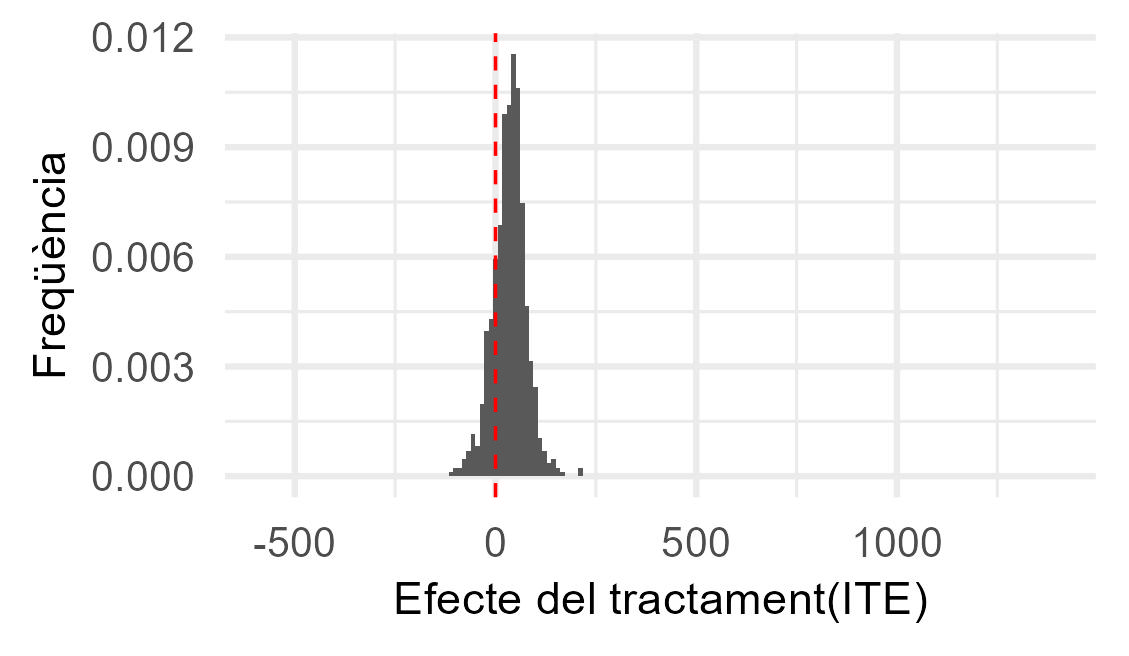
\includegraphics[width=0.3\textwidth]{imgs/histogrames/hist(PesoRN)S_tract2.jpg} &
    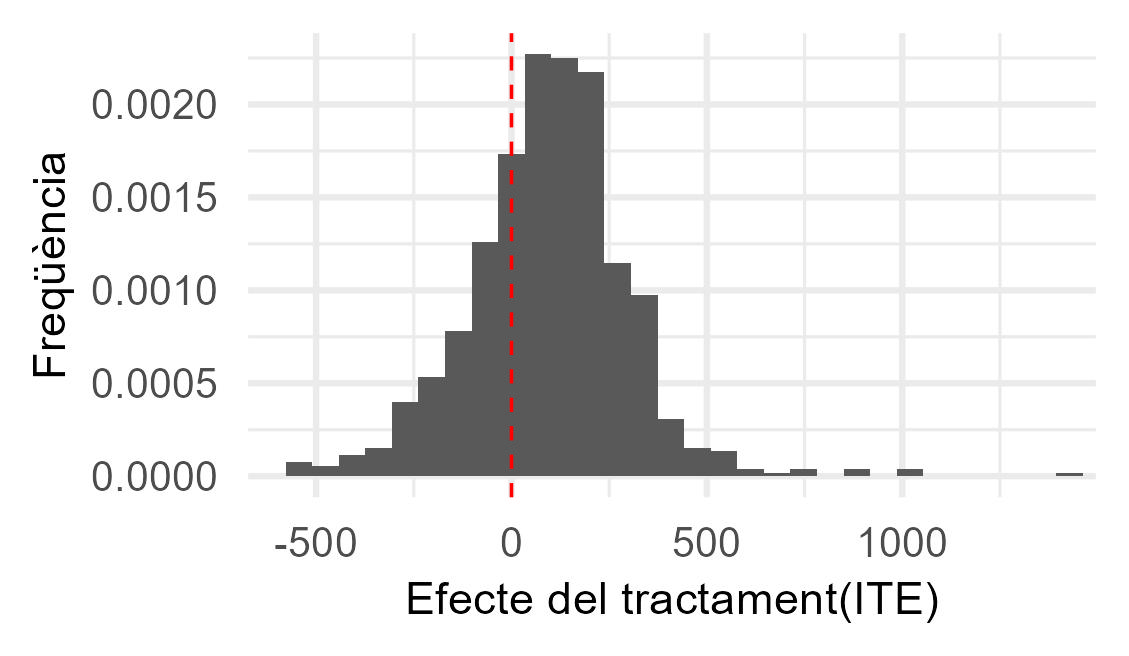
\includegraphics[width=0.3\textwidth]{imgs/histogrames/hist(PesoRN)T_tract2.jpg} &
    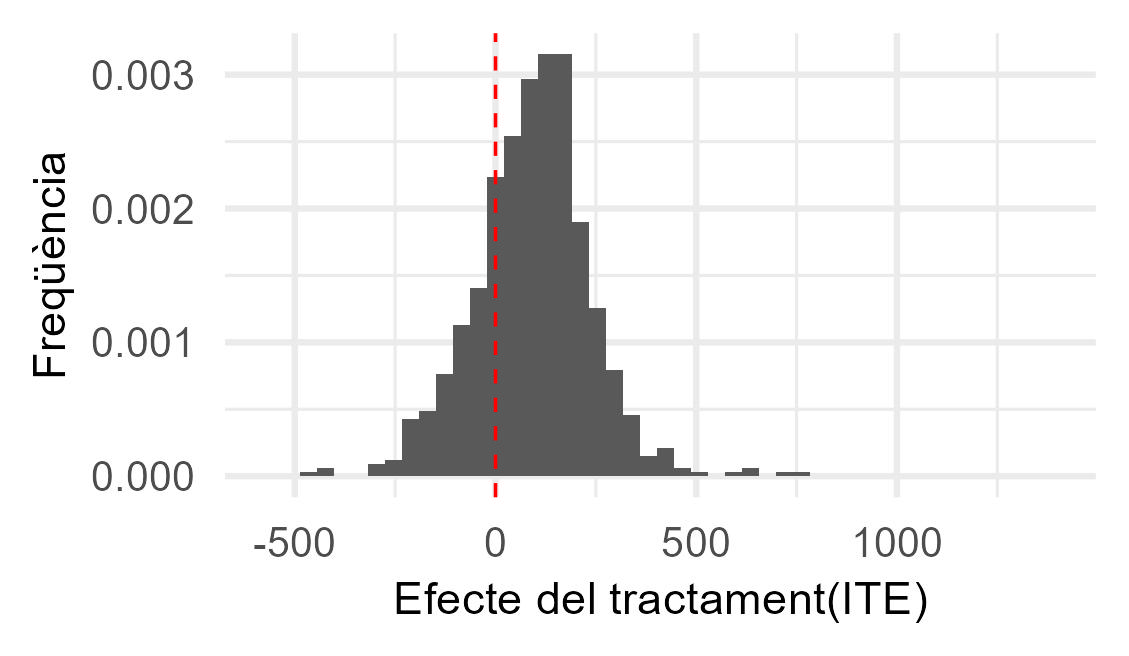
\includegraphics[width=0.3\textwidth]{imgs/histogrames/hist(PesoRN)X_tract2.jpg} \\
    \end{tabular}
    \caption{\footnotesize Comparació dels ITEs i ATE estimats amb S-, T- i X-learner per la variable resposta \textit{pes del nadó al naixement}}
    \label{tab:histITE_pes2}
    \end{table}
    
    En aquest context, l’anàlisi dels ATEs mostra que l’estratègia de dieta mediterrània produeix un increment del pes mitjà, amb resultats consistents entre els tres meta-learners, que estimen un efecte positiu del tractament sobre aquesta variable.


%histogrames reducció d'estrès
    \begin{table}[H]
    \centering
    \begin{tabular}{ccc}
    \multicolumn{3}{c}{Histograma de l'ITE amb \textbf{reducció estrès}} \\
    \small \textbf{S-learner} & \small \textbf{T-learner} & \small\textbf{X-learner} \\
    \footnotesize ATE = 35.67 & \footnotesize ATE = 93.60 & \footnotesize ATE = 95.53 \\
    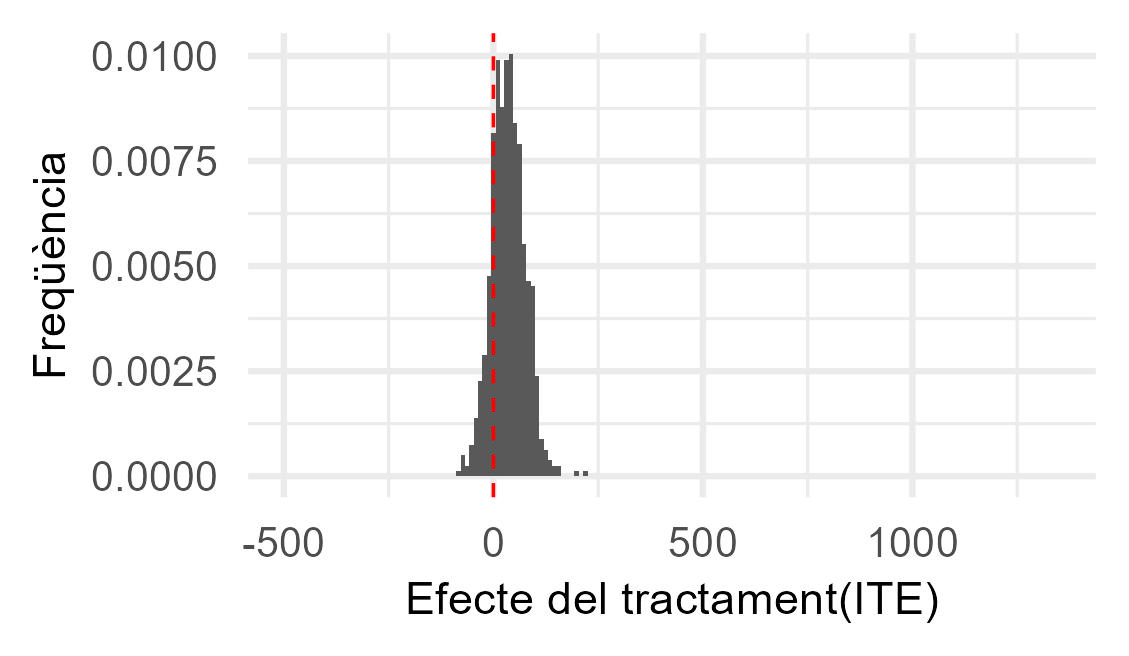
\includegraphics[width=0.3\textwidth]{imgs/histogrames/hist(PesoRN)S_tract3.jpg} &
    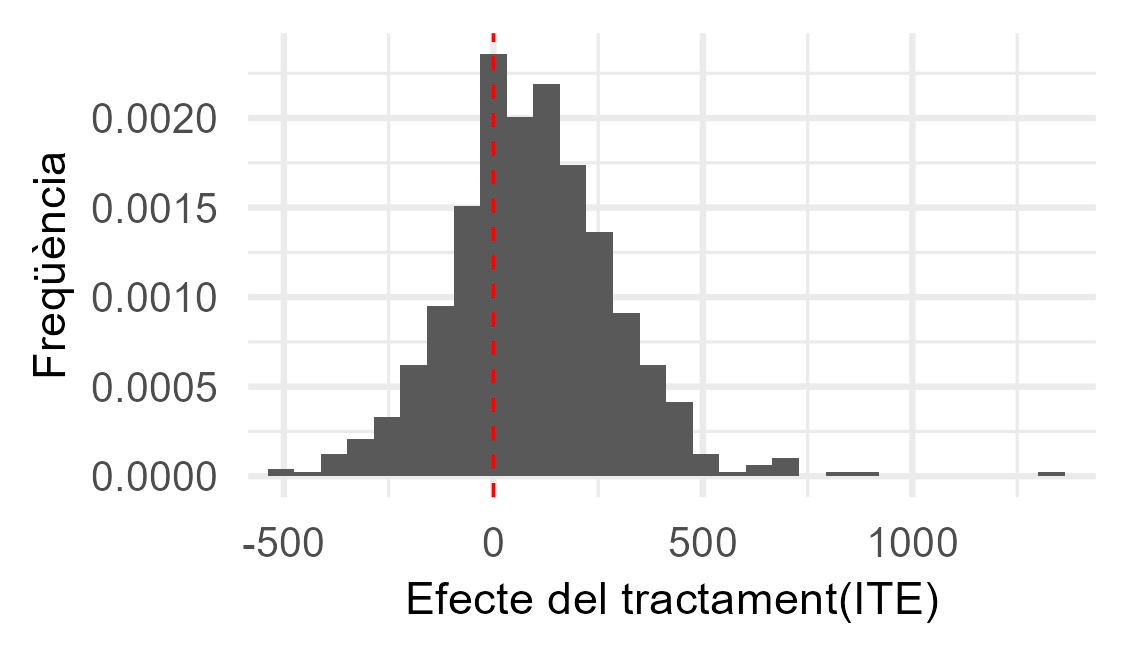
\includegraphics[width=0.3\textwidth]{imgs/histogrames/hist(PesoRN)T_tract3.jpg} &
    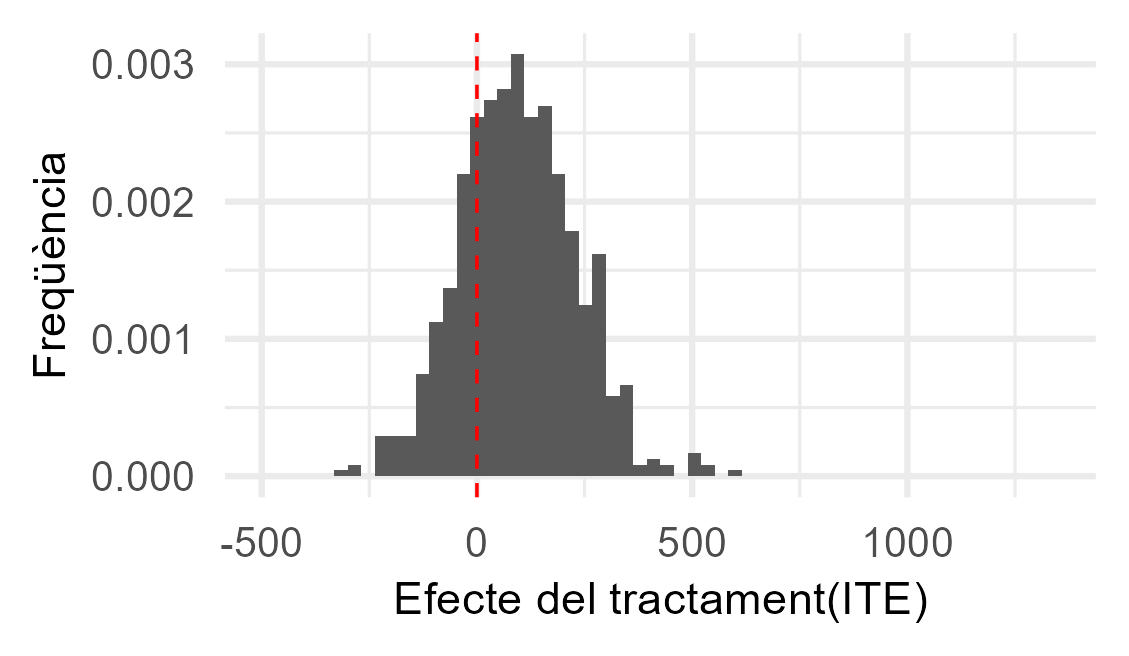
\includegraphics[width=0.3\textwidth]{imgs/histogrames/hist(PesoRN)X_tract3.jpg} \\
    \end{tabular}
    \caption{\footnotesize Comparació visual dels ITEs i ATE estimats amb S-, T- i X-learner per la variable resposta \textit{pes del nadó al naixement}}
    \label{tab:histITE_pes3}
    \end{table}

    El comportament observat amb el tractament de reducció de l'estrès és molt similar al del tractament anterior, ja que seguir aquesta estratègia també mostra un efecte clarament positiu sobre el pes al naixement.\par
    D’altra banda, si ens fixem en les distribucions dels ITEs estimades pels tres meta-learners (tant per a la reducció de l’estrès com per a la dieta mediterrània), s’observa que la del T-learner és considerablement més dispersa, indicant una major variabilitat en els efectes estimats entre individus. \footnote{Tots els histogrames es divideixen en 30 blocs, en el cas del T-learner aquests son més amples ja que abarquen més espai cosa que també fa que sigui els que té menys altura i per tant una distibució més aplanada. Cal remarcar que l’escala de l’eix X és la mateixa per a tots els histogrames dins d’un mateix tractament, però l’escala de l’eix Y no ho és, fet que pot influir en la percepció visual de les diferències entre distribucions.}

%taula coeficients
    \begin{table}[H]
        \centering
        \captionsetup{font=small}
        \caption{Coeficients estimats i intervals de confiança model lineal per CATE de pes al naixement}
        \label{tab:coef_pesRN}
        \centering
        \scriptsize
        \begin{tabular}[t]{p{4cm} c @{\hspace{1cm}} c}
        \toprule
        Variable & Tractament  & Tractament \\
         & Dieta mediterrània & Reducció estrès \\
        \midrule
        (Intercept) & \textbf{-800.90 (-1027.19; -574.61)} & \textbf{-1301.46 (-1528.73; -1074.20)}\\
        Edat & \textbf{6.18 (4.40; 7.97)} & \textbf{5.37 (3.63; 7.10)}\\
        Talla & \textbf{3.65 (2.36; 4.93)} & \textbf{6.57 (5.28; 7.85)}\\
        IMC pregestacional & \textbf{2.65 (0.90; 4.40)} & \textbf{3.43 (1.77; 5.09)}\\
        Fumadora & -10.64 (-86.47; 65.18) & -3.77 (-61.68; 54.13)\\
        \addlinespace
        Antecedents SGA & -13.98 (-39.21; 11.24) & 9.19 (-16.68; 35.05)\\
        HTA crònica & \textbf{115.17 (73.84; 156.50)} & -28.84 (-68.75; 11.07)\\
        Diabetis gestacional & 7.52 (-31.54; 46.57) & 26.08 (-12.91; 65.06)\\
        Nefropatia & \textbf{-62.60 (-119.88; -5.32)} & 22.32 (-32.13; 76.77)\\
        Malaltia autoimmune & \textbf{-77.35 (-100.11; -54.59)} & -14.04 (-36.52; 8.44)\\
        \addlinespace
        Doppler patològic & \textbf{-189.82 (-227.00; -152.64)} & \textbf{-132.44 (-167.10; -97.77)}\\
        Risc PE & \textbf{106.41 (87.40; 125.43)} & \textbf{30.53 (11.51; 49.54)}\\
        PAPP-A patològic & 12.46 (-23.61; 48.53) & \textbf{103.32 (67.36; 139.29)}\\
        Metrorràgia & \textbf{-187.89 (-227.68; -148.10)} & \textbf{-49.51 (-85.39; -13.62)}\\
        Criteris SGA & 12.38 (-8.66; 33.41) & \textbf{26.70 (5.94; 47.47)}\\
        \addlinespace
        Fecundació assistida & \textbf{-24.82 (-46.71; -2.93)} & \textbf{-70.57 (-92.23; -48.92)}\\
        Nul·liparitat & 12.43 (-8.33; 33.18) & \textbf{88.01 (67.44; 108.59)}\\
        \bottomrule
        \multicolumn{3}{l}{\rule{0pt}{1em} *coef ($IC_{95\%}$); \textit{Amb negreta les variables significatives amb $\alpha=0.05$}}
        \end{tabular}
    \end{table}

    Pel que fa als coeficients del model multivariant amb totes les característiques de la mare (taula \ref{tab:coef_pesRN}) s'observa que en \textbf{ambdós tractaments}, les tres covariables numèriques -\textit{edat}, \textit{talla} i \textit{BMI pregestacional}- estan associades a un augment de l’efecte del tractament. Això indica que el benefici del tractament és major en mares amb valors més elevats d’aquestes variables. Així mateix, la presència de \textit{risc clínic de preeclàmpsia} també s’associa a una millora notable de l’efecte estimat.\par
    Per contra, altres factors com la \textit{detecció de patologies en l’ecografia Doppler del primer trimestre}, la \textit{metrorràgia} i el fet que l’embaràs hagi estat \textit{concebut mitjançant tècniques de reproducció assistida (TRA)} es relacionen, en general, amb una disminució de l’efectivitat del tractament, tant en el grup de dieta mediterrània com en el de reducció d'estrès.\par
    Entrant en el detall de cada tractament, en el cas de la \textbf{dieta mediterrània}, destaca especialment l’efecte positiu de l’\textit{edat} i de la \textit{hipertensió arterial crònica}, que amplifiquen significativament l’impacte del tractament. Tanmateix, la presència de \textit{nefropatia} i de \textit{malalties autoimmunitàries} redueixen l’efecte estimat, i la \textit{detecció ecogràfica de patologia uterina} o la \textit{metrorràgia} tenen també un impacte clarament negatiu.\par
    Pel que fa a la \textbf{reducció de l'estrès}, s’observa que la \textit{talla materna elevada} i la presència de \textit{valors patològics de la proteïna PAPP-A} potencien l’efecte del tractament. A més, cal destacar que ser \textit{nul·lípara} (primer embaràs) també s’associa a una resposta més favorable a aquest tractament.\par

    % \begin{figure}[htb]
    %   \centering
    %   \begin{minipage}[b]{0.48\textwidth}
    %     \includegraphics[width=\textwidth]{imgs/scaterplots/scater_PesoRN_2_EdatMetrorragia.jpg}
    %     \scriptsize\caption{ITE en el pes del nounat amb tractmaent de \textbf{dieta mediterrània} en funció de l'\textit{edat} diferenciant per \textit{metrorràgia}}
    %     \label{plot:peso2}
    %   \end{minipage}
    %   \hspace{0.01\textwidth}
    %   \begin{minipage}[b]{0.48\textwidth}
    %     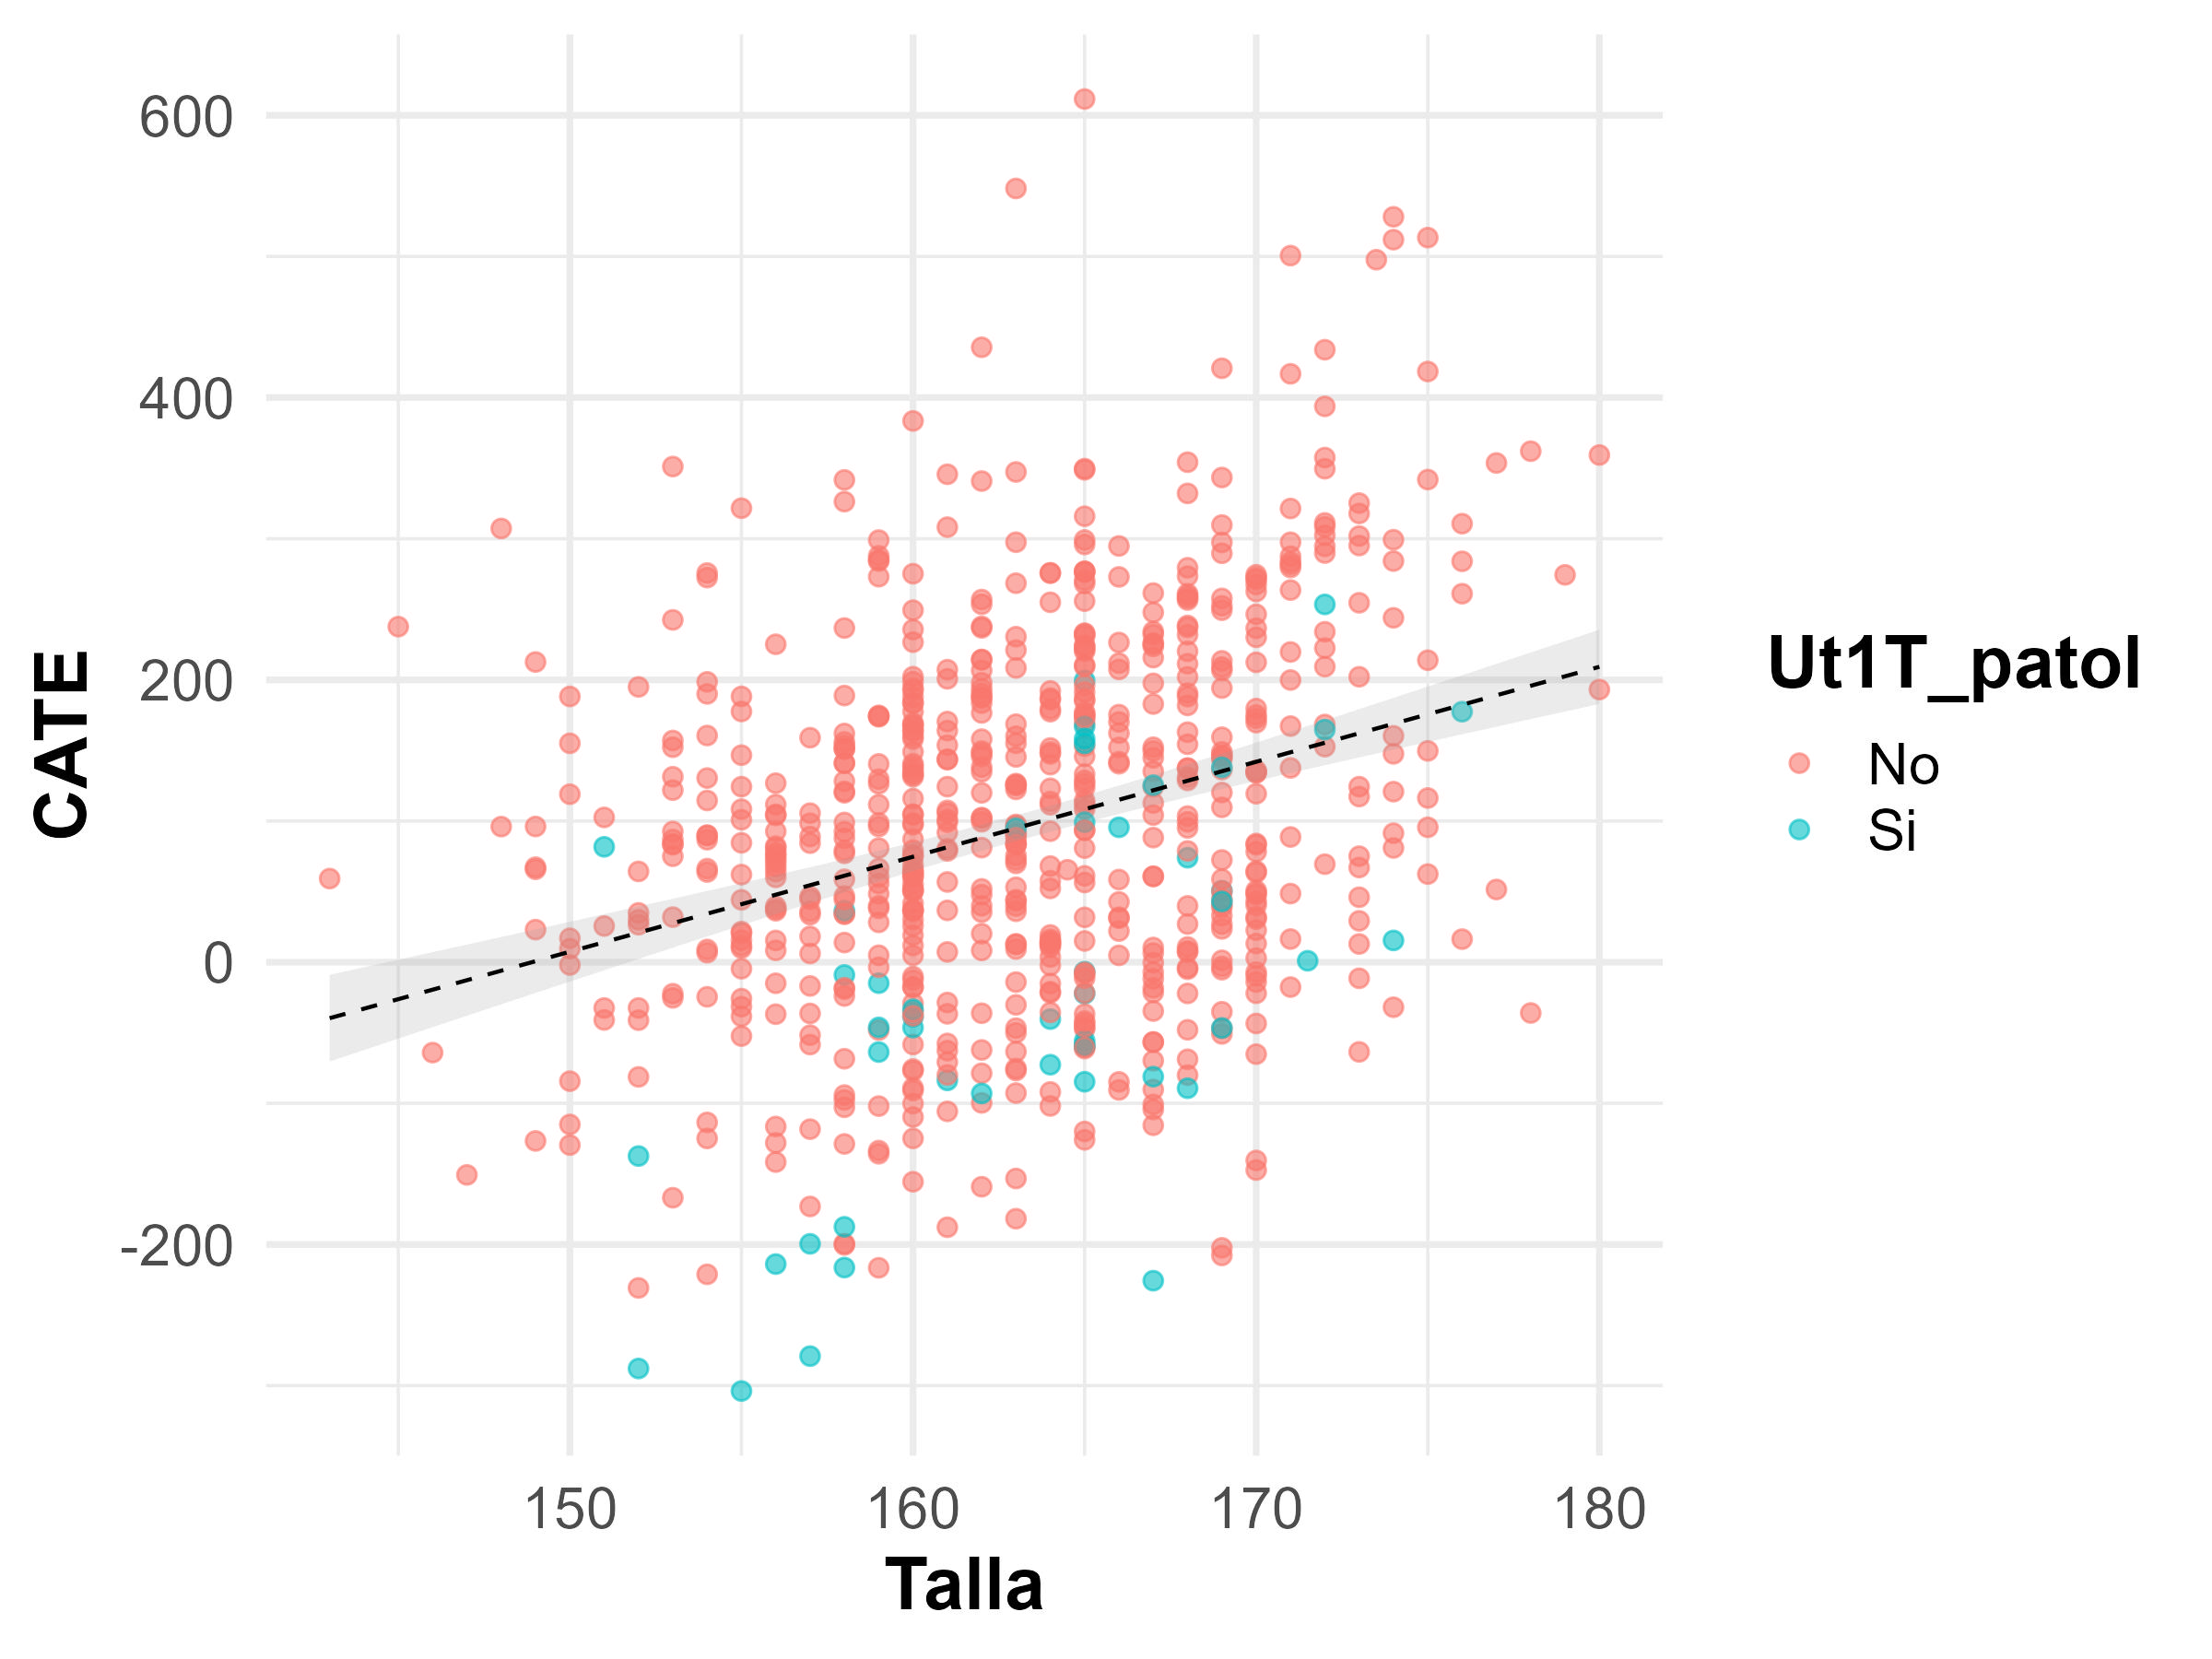
\includegraphics[width=\textwidth]{imgs/scaterplots/scater_PesoRN_3_TallaUt1T.jpg}
    %     \caption{ITE en el pes del nounat amb tractmaent de \textbf{Reducció d'estrès} en funció de \textit{talla} diferenciant per \textit{hipertensió arterial}}
    %   \end{minipage}
    % \end{figure}
    
    %Per dieta mediterrania destaca especialement l'efecte de l'edat i  l'hipertensió cronica positivament i el diagnosis a l'ecografia de Doppler i la metorragia negativament. Mentre per la Reducció d'estrès en positiu hi ha la Tall i el nivell patologic de PAPPA i en negatiu destaca la diagnosis positiva a la ecografia de Doppler


    \FloatBarrier
    \subsection{Percentil de pes al naixement}\label{subsec:percentil}
    El percentil del pes al naixement és una altra variable estretament relacionada amb el desenvolupament del nadó. En aquest cas, el percentil indica en quin punt es troba el pes del nadó en relació amb la resta de la població de referència per edat gestacional i sexe. Com en el cas del pes absolut, un efecte positiu del tractament sobre aquesta variable es pot interpretar com un millor desenvolupament fetal, ja que el nadó es situaria en percentils més elevats.

    
%histogrames amb dieta mediterrània
    \begin{table}[H]
        \centering
        \begin{tabular}{ccc}
        \multicolumn{3}{c}{Histograma de l'ITE amb \textbf{dieta mediterrània}} \\
        \small \textbf{S-learner} & \small \textbf{T-learner} & \small \textbf{X-learner} \\
        \footnotesize ATE = 0.67 & \footnotesize ATE = 2.28 & \footnotesize ATE = 2.24 \\
        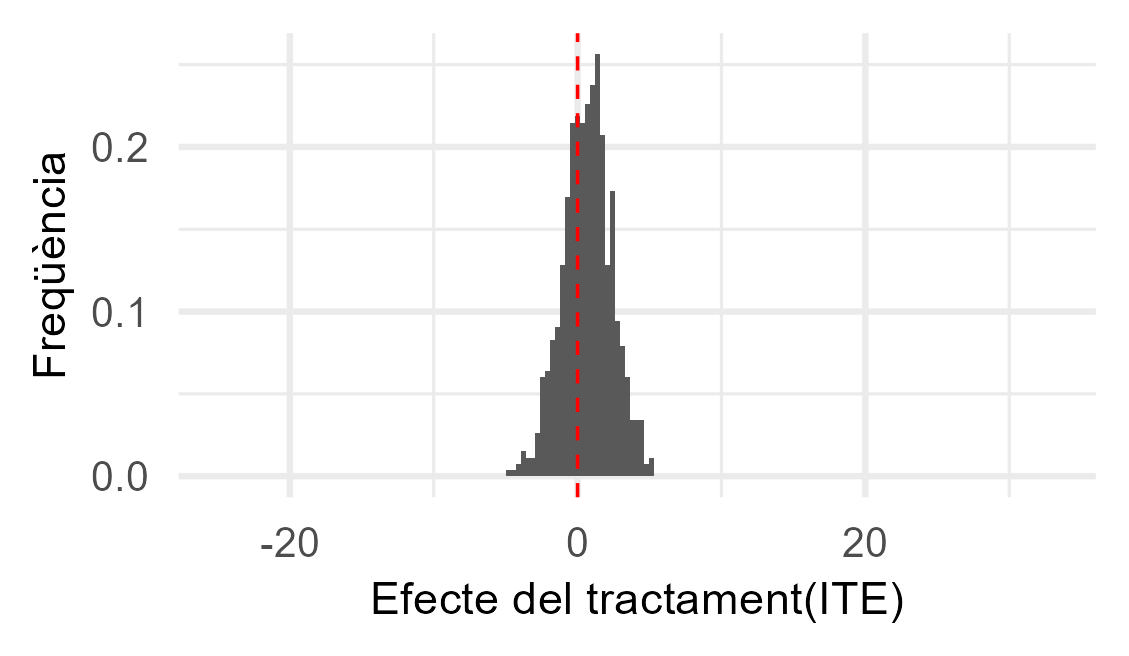
\includegraphics[width=0.3\textwidth]{imgs/histogrames/hist(percentil_birth)S_tract2.jpg} &
        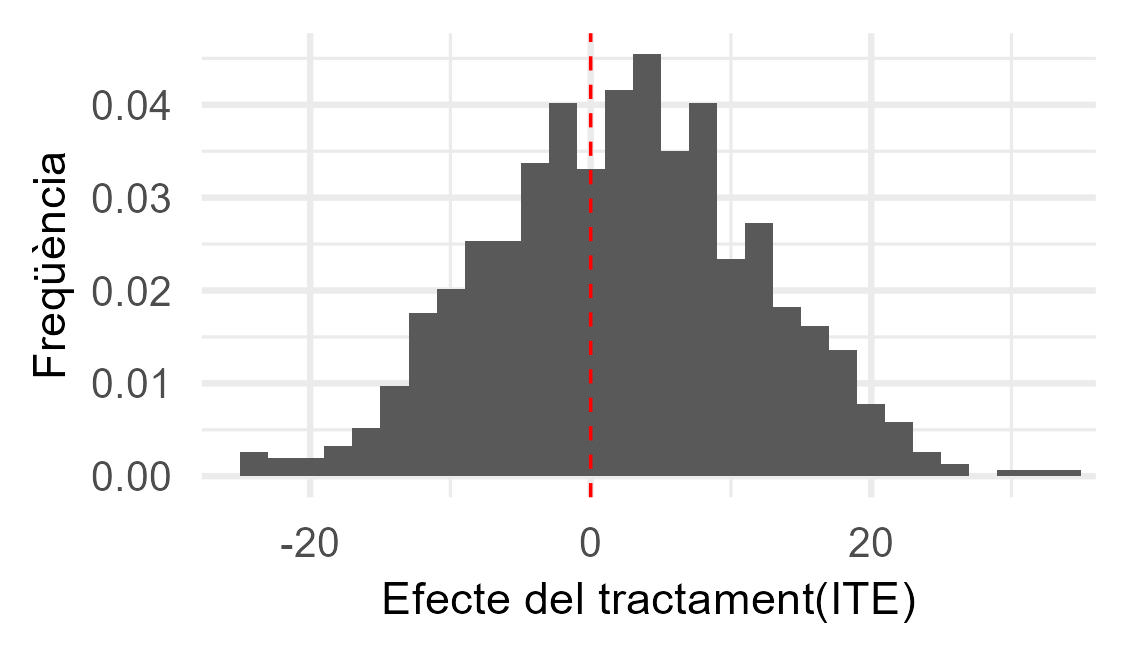
\includegraphics[width=0.3\textwidth]{imgs/histogrames/hist(percentil_birth)T_tract2.jpg} &
        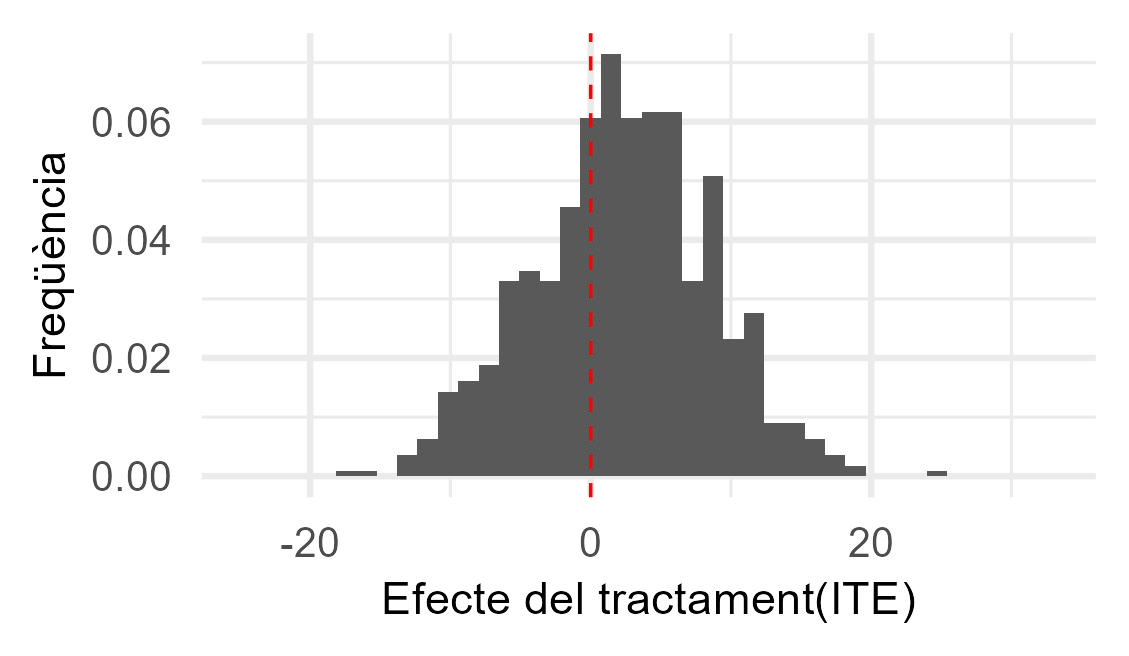
\includegraphics[width=0.3\textwidth]{imgs/histogrames/hist(percentil_birth)X_tract2.jpg} \\
        \end{tabular}
        \footnotesize \caption{\footnotesize Comparació visual dels ITEs i ATE estimats amb S-, T- i X-learner per la variable resposta \textit{percentil de pes al naixement}}
        \label{tab:histITE_percentil2}
    \end{table}

    Novament, s’observa que els tres meta-learners generen distribucions força diferents. L’S-learner presenta una distribució molt concentrada i propera a zero, mentre que el T-learner mostra una variabilitat més gran, amb una distribució més àmplia. L’X-learner adopta una forma similar a la del T-learner, però amb una dispersió lleugerament menor. Si ens fixem en l’ATE estimat amb l’X-learner, el més robust dels tres, veiem que el tractament de reducció de l’estrès augmentaria de mitjana en 2.24 punts el percentil de pes al naixement.

%histogrames reducció d'estrès
    \begin{table}[H]
        \centering
        \begin{tabular}{ccc}
        \multicolumn{3}{c}{Histograma de l'ITE amb \textbf{reducció estrès}} \\
        \small \textbf{S-learner} & \small \textbf{T-learner} & \small \textbf{X-learner} \\
        \footnotesize ATE = 1.13 & \footnotesize ATE = 2.41 & \footnotesize ATE = 2.33 \\
        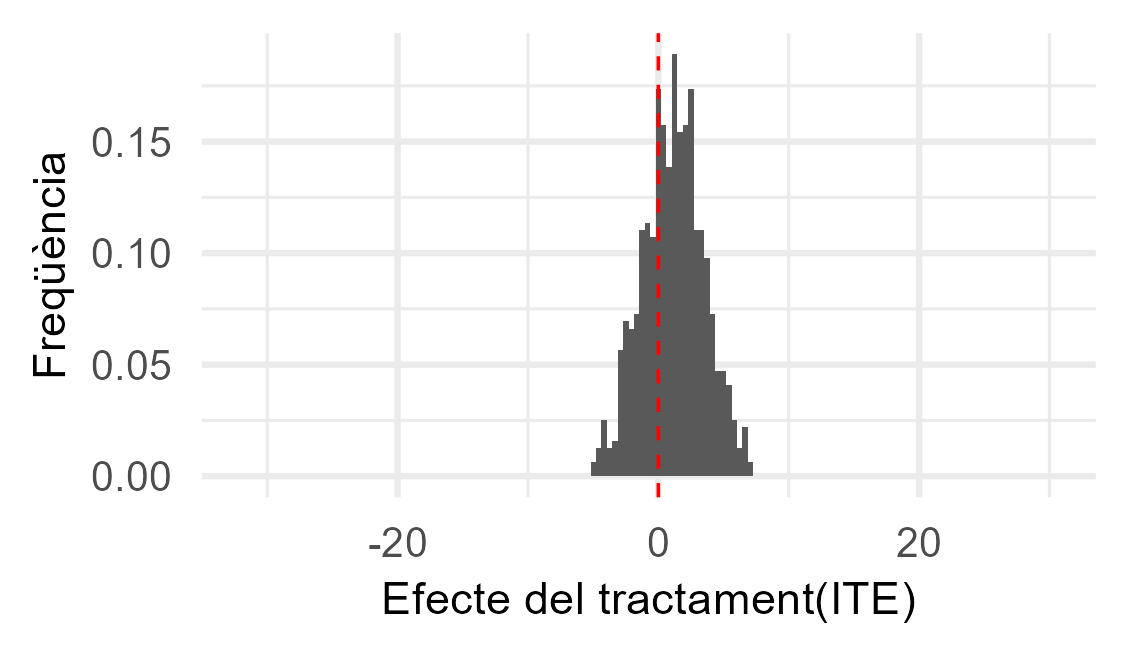
\includegraphics[width=0.3\textwidth]{imgs/histogrames/hist(percentil_birth)S_tract3.jpg} &
        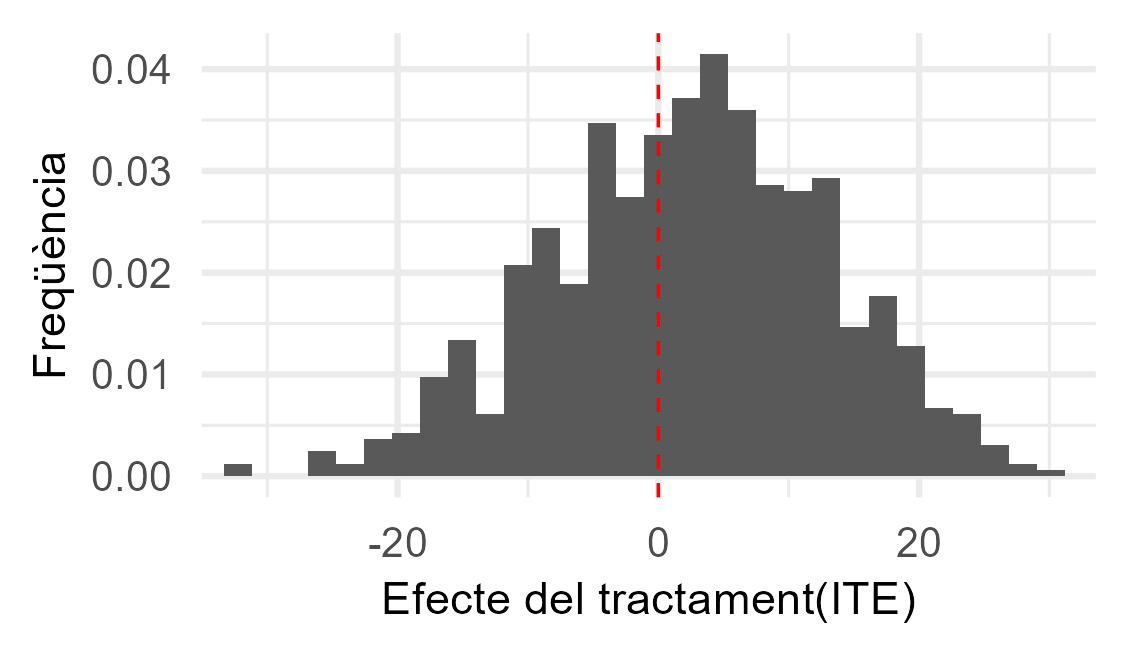
\includegraphics[width=0.3\textwidth]{imgs/histogrames/hist(percentil_birth)T_tract3.jpg} &
        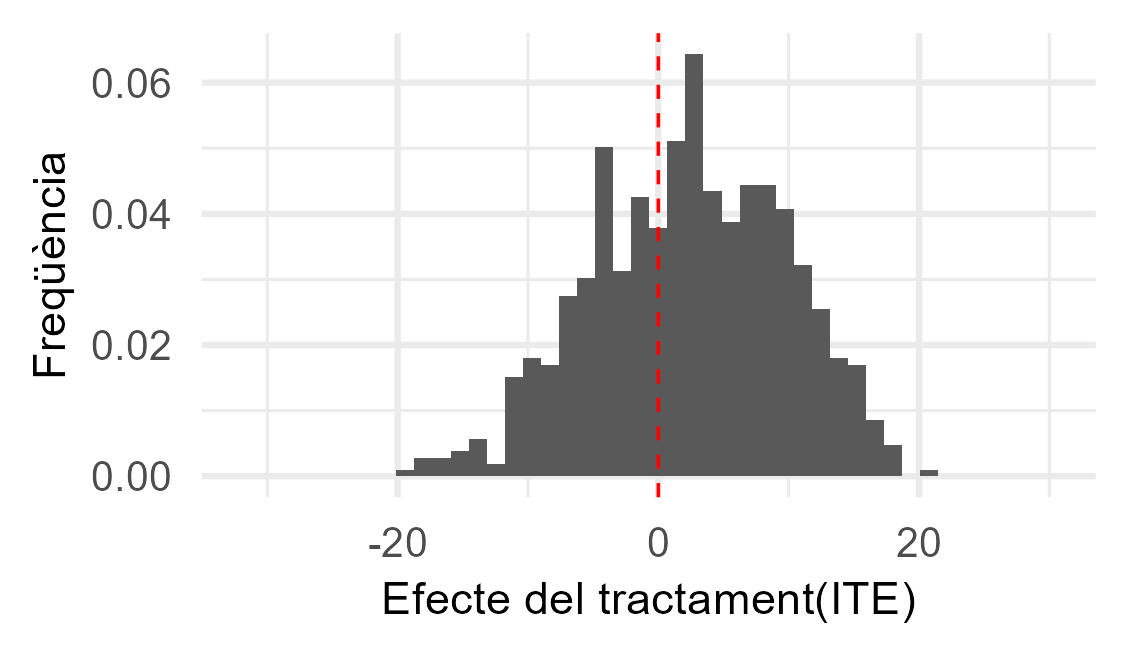
\includegraphics[width=0.3\textwidth]{imgs/histogrames/hist(percentil_birth)X_tract3.jpg} \\
        \end{tabular}
        \caption{\footnotesize Comparació visual dels ITEs i ATE estimats amb S-, T- i X-learner per la variable resposta \textit{percentil de pes al naixement}}
        \label{tab:histITE_percentil3}
    \end{table}

    Pel que fa a la reducció d'estrès, les distribucions dels ITEs són similars a les del tractament anterior, mantenint una forma propera a la normalitat, amb diferències d’amplada i altura entre models. En aquest cas, però, tant el T-learner com l’X-learner mostren lleugeres acumulacions a la banda negativa de l’ATE, tot i que la mitjana es manté clarament positiva. L’ATE estimat per l’X-learner és de +2,33, indicant que aquest tractament també tindria un efecte beneficiós sobre el percentil de pes, encara que suggereix una lleugera asimetria en la resposta individual.


%taula coeficients
    \begin{table}[H]
        \centering
        \captionsetup{font=small}
        \caption{Coeficients estimats i intervals de confiança model lineal per CATE de percentil de pes}
        \centering
        \scriptsize
        \label{tab:coef_percentil}
        \begin{tabular}[t]{p{4cm} c @{\hspace{1cm}} c}
        \toprule
        Variable & Tractament  & Tractament \\
         & Dieta mediterrània & Reducció estrès \\
        \midrule
        (Intercept) & 1.91 (-9.19; 13.01) & \textbf{-54.59 (-66.47; -42.72)}\\
        Edat & \textbf{-0.17 (-0.26; -0.08)} & \textbf{0.10 (0.01; 0.19)}\\
        Talla & \textbf{0.07 (0.00; 0.13)} & \textbf{0.28 (0.22; 0.35)}\\
        IMC pregestacional & \textbf{-0.24 (-0.32; -0.15)} & \textbf{0.13 (0.05; 0.22)}\\
        Fumadora & \textbf{-6.06 (-9.78; -2.34)} & \textbf{-10.59 (-13.62; -7.57)}\\
        \addlinespace
        Antecedents SGA & 1.14 (-0.10; 2.38) & \textbf{3.32 (1.96; 4.67)}\\
        HTA crònica & \textbf{2.60 (0.57; 4.63)} & -0.01 (-2.10; 2.08)\\
        Diabetis gestacional & 1.61 (-0.31; 3.52) & 0.42 (-1.61; 2.46)\\
        Nefropatia & \textbf{-10.02 (-12.83; -7.21)} & \textbf{-5.84 (-8.68; -2.99)}\\
        Malaltia autoimmune & \textbf{-3.44 (-4.56; -2.33)} & -0.34 (-1.51; 0.84)\\
        \addlinespace
        Doppler patològic & \textbf{-5.11 (-6.93; -3.28)} & \textbf{-2.70 (-4.51; -0.89)}\\
        Risc PE & \textbf{1.54 (0.61; 2.47)} & \textbf{-1.53 (-2.53; -0.54)}\\
        PAPP-A patològic & -0.45 (-2.22; 1.32) & \textbf{7.98 (6.10; 9.86)}\\
        Metrorràgia & \textbf{-2.97 (-4.93; -1.02)} & \textbf{-6.02 (-7.90; -4.15)}\\
        Criteris SGA & \textbf{1.13 (0.10; 2.16)} & \textbf{2.18 (1.10; 3.27)}\\
        \addlinespace
        Fecundació assistida & 0.18 (-0.90; 1.25) & \textbf{-1.67 (-2.80; -0.54)}\\
        Nul·liparitat & \textbf{1.95 (0.94; 2.97)} & \textbf{6.05 (4.98; 7.13)}\\
        \bottomrule
        \multicolumn{3}{l}{\rule{0pt}{1em}*coef ($IC_{95\%}$); \textit{Amb negreta les variables significatives amb $\alpha=0.05$}}
        \end{tabular}
    \end{table}

    Si ens fixem amb els coeficients del model lineal de la taula \ref{tab:coef_percentil} S’observa que \textit{fumar durant l’embaràs}, la presència de \textit{nefropatia}, la d\textit{etecció de patologia mitjançant ecografia Doppler} i la \textit{metrorràgia} redueixen l’efecte del tractament tant en el cas de la reducció de l’estrès com en el de la reducció d'estrès. A nivell positiu, només es detecta l'efecte favorable compartit per ambdós tractaments en el cas de la \textit{talla} materna (tot i que de manera més modesta per a la reducció de l’estrès) i de la \textit{nul·liparitat}, que es relaciona amb una resposta més intensa al tractament.\par
    Focalitzant-nos en el tractament de \textbf{dieta mediterrània}, més enllà dels efectes comuns ja comentats, cal destacar l’impacte negatiu de la presència de \textit{malalties autoimmunitàries}. En canvi, les pacients amb \textit{hipertensió arterial crònica} o \textit{risc clínic de preeclàmpsia} experimenten un efecte positiu superior, suggerint una resposta favorable més marcada en aquests subgrups.\par
    En el cas de la \textbf{reducció d'estrès}, els resultats mostren en general una major heterogeneïtat en la resposta. A més dels efectes compartits amb l’altre tractament, es detecta una reducció de l’efecte en mares amb \textit{risc de preeclàmpsia} i en \textit{embarassos concebuts mitjançant tècniques de reproducció assistida (TRA)}. Per contra, l’efecte s’incrementa significativament en mares amb \textit{antecedents de SGA}, amb valors \textit{patològics de la proteïna PAPP-A} o que compleixen \textit{criteris clínics menors de risc d’SGA}, la qual cosa podria indicar una major utilitat d’aquest tractament en perfils de més risc de SGA.



    \subsection{SGA al naixement}\label{subsec:SGAneix}

    La presència de SGA al naixement és la variable resposta principal de l’estudi original, ja que constitueix un indicador directe del desenvolupament fetal i, per extensió, de la qualitat i l’evolució de l’embaràs. En aquest context, una reducció en la taxa de SGA s’interpreta com un efecte beneficiós del tractament aplicat.

    
%histogrames amb dieta mediterrània
    \begin{table}[H]
        \centering
        \begin{tabular}{ccc}
        \multicolumn{3}{c}{Histograma de l'ITE amb \textbf{dieta mediterrània}} \\
        \small \textbf{S-learner} & \small \textbf{T-learner} & \small \textbf{X-learner} \\
        \footnotesize ATE = -0.029 & \footnotesize ATE = -0.077 & \footnotesize ATE = -0.073 \\
        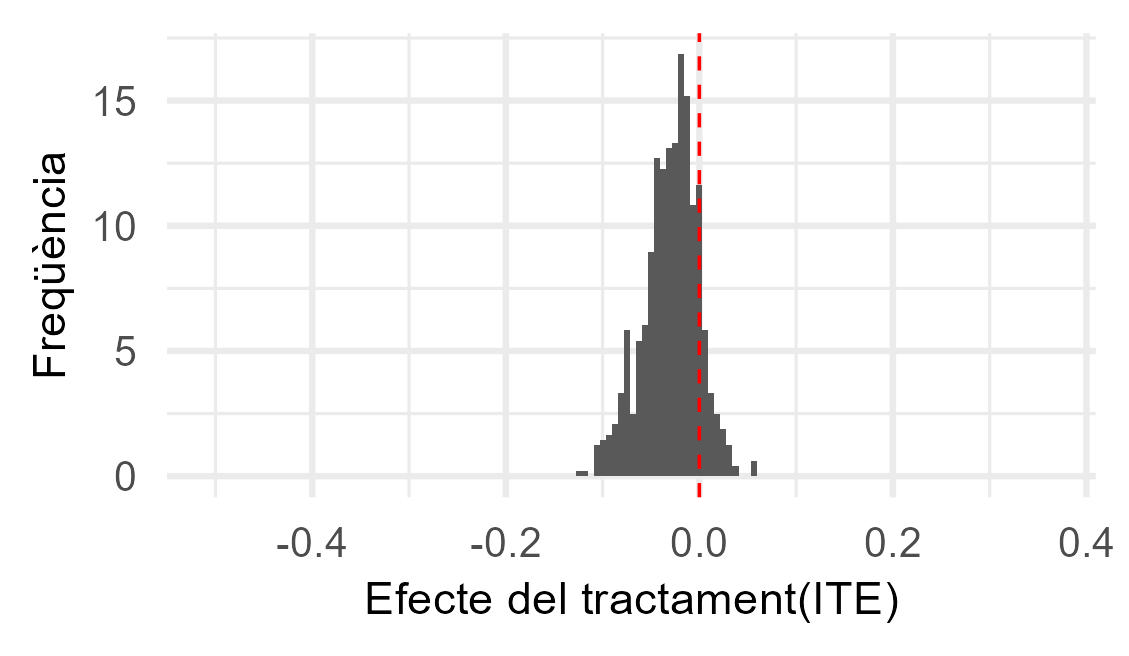
\includegraphics[width=0.3\textwidth]{imgs/histogrames/hist(SGA_birth_hard_imput)S_tract2.jpg} &
        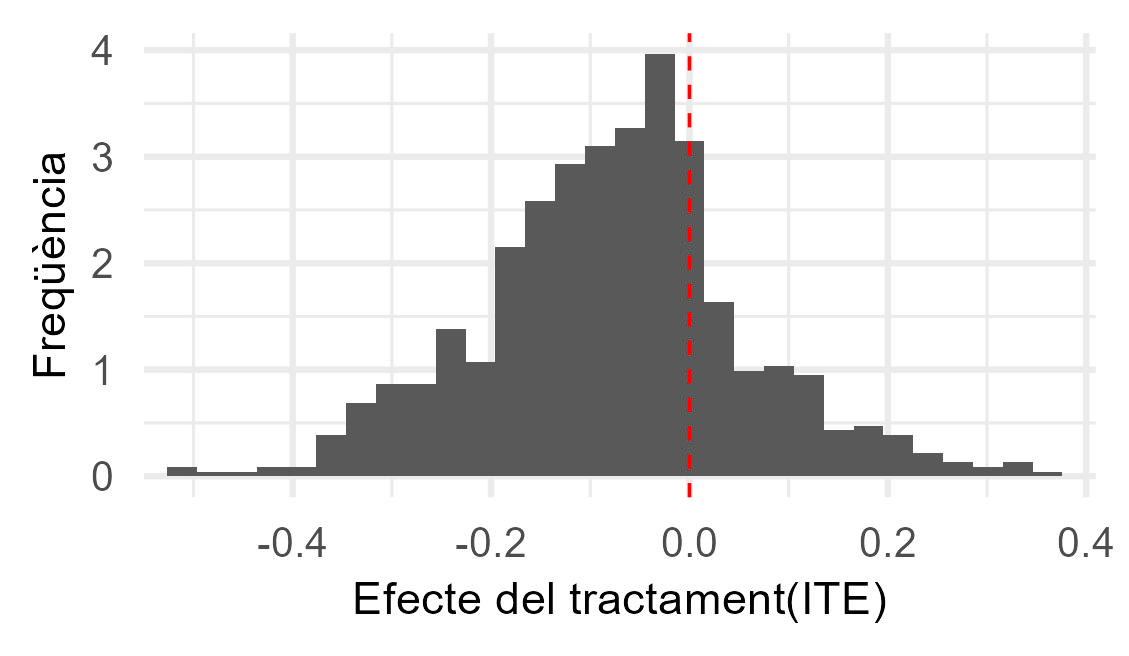
\includegraphics[width=0.3\textwidth]{imgs/histogrames/hist(SGA_birth_hard_imput)T_tract2.jpg} &
        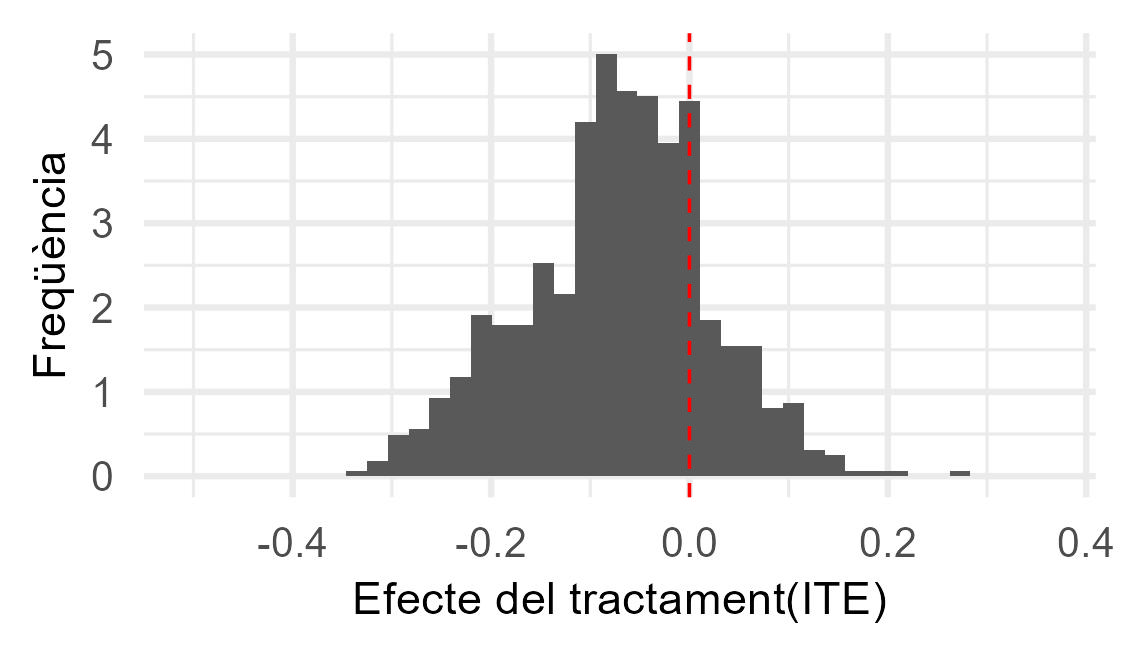
\includegraphics[width=0.3\textwidth]{imgs/histogrames/hist(SGA_birth_hard_imput)X_tract2.jpg} \\
        \end{tabular}
        \caption{\footnotesize Comparació visual dels ITEs i ATE estimats amb S-, T- i X-learner per la variable resposta \textit{SGA al naixement}}
        \label{tab:histITE_SGAneix2}
    \end{table}

    Tot i que els valors de l’ATE es troben dins un rang de valors més petits que les variables anteriors, les distribucions dels ITEs mostren patrons similars. Pel que fa al tractament de dieta mediterrània, l’efecte mitjà estimat amb l’X-learner indica una disminució aproximada del 7,3\% en la probabilitat de SGA, evidenciant un impacte positiu del tractament en termes de creixement fetal.


%histogrames reducció d'estrès
    \begin{table}[H]
        \centering
        \begin{tabular}{ccc}
        \multicolumn{3}{c}{Histograma de l'ITE amb \textbf{reducció estrès}} \\
        \small \textbf{S-learner} & \small \textbf{T-learner} & \small \textbf{X-learner} \\
        \footnotesize ATE = -0.027 & \footnotesize ATE = -0.065 & \footnotesize ATE = -0.061 \\
        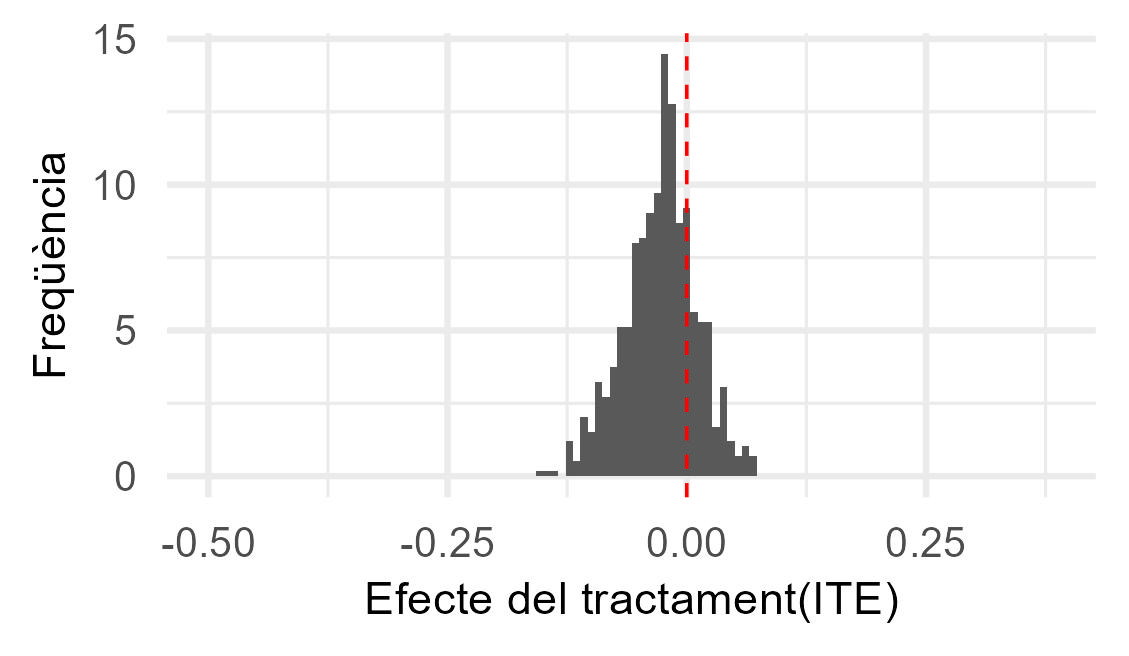
\includegraphics[width=0.3\textwidth]{imgs/histogrames/hist(SGA_birth_hard_imput)S_tract3.jpg} &
        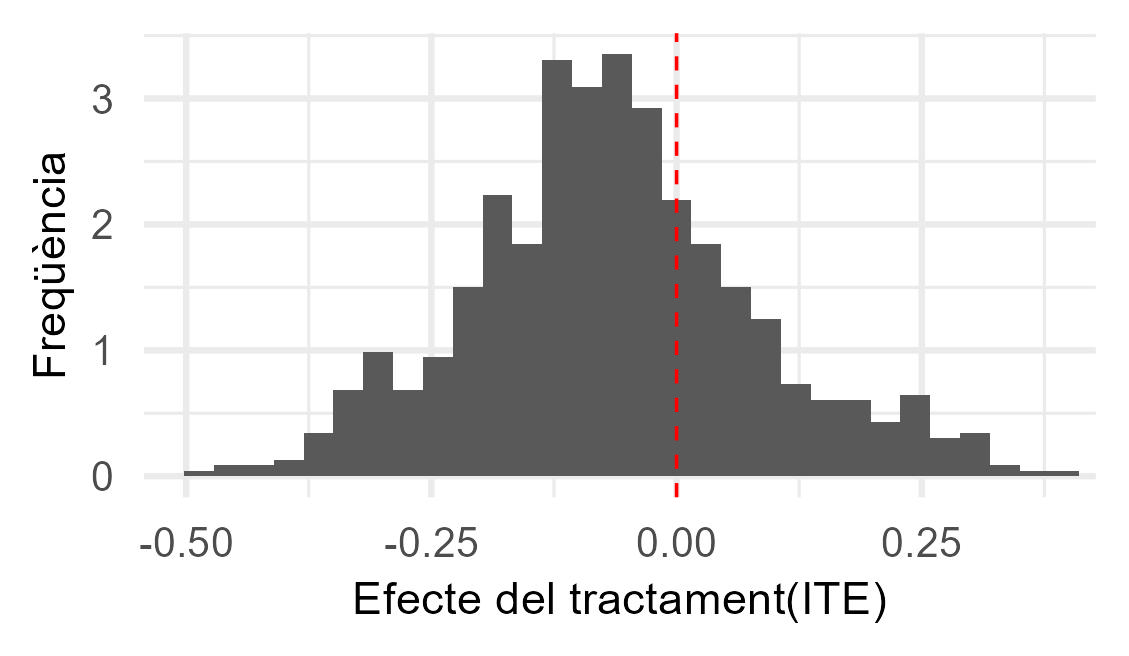
\includegraphics[width=0.3\textwidth]{imgs/histogrames/hist(SGA_birth_hard_imput)T_tract3.jpg} &
        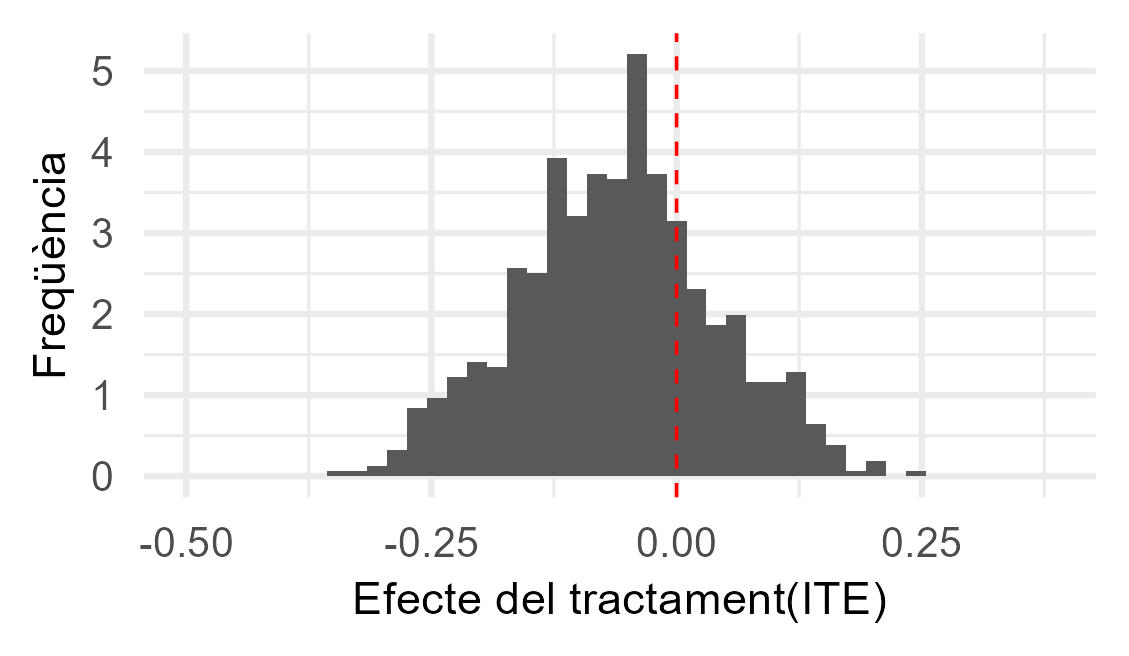
\includegraphics[width=0.3\textwidth]{imgs/histogrames/hist(SGA_birth_hard_imput)X_tract3.jpg} \\
        \end{tabular}
        \caption{\footnotesize Comparació visual dels ITEs i ATE estimats amb S-, T- i X-learner per la variable resposta \textit{SGA al naixement}}
        \label{tab:histITE_SGAneix3}
    \end{table}

    Amb el tractament de reducció d'estrès, les distribucions de l’ITE són molt similars a les del cas anterior. L’ATE estimat pel X-learner és de -0.061, indicant una reducció mitjana del 6.1\% en la incidència de SGA. També s’observa que, en ambdós tractaments, el T-learner tendeix a produir valors mitjans més extrems que el X-learner.

%taula coeficients
    \begin{table}[H]
        \centering
        \captionsetup{font=small}
        \caption{Coeficients estimats i intervals de confiança del model lineal per CATE de SGA al naixement}
        \label{tab:coef_SGAnaix}
        \centering
        \scriptsize
        \begin{tabular}[t]{p{4cm} c @{\hspace{1cm}} c}
        \toprule
        Variable & Tractament  & Tractament \\
         & Dieta mediterrània & Reducció estrès \\
        \midrule
        (Intercept) & 0.03 (-0.11; 0.17) & \textbf{0.75 (0.61; 0.90)}\\
        Edat & \textbf{0.00 (0.00; 0.00)} & \textbf{0.01 (0.00; 0.01)}\\
        Talla & \textbf{-0.00 (-0.00; -0.00)} & \textbf{-0.01 (-0.01; -0.01)}\\
        IMC pregestacional & \textbf{0.00 (0.00; 0.00)} & \textbf{-0.00 (-0.00; -0.00)}\\
        Fumadora & -0.00 (-0.05; 0.05) & \textbf{0.06 (0.02; 0.10)}\\
        \addlinespace
        Antecedents SGA & -0.01 (-0.03; 0.00) & \textbf{0.04 (0.02; 0.06)}\\
        HTA crònica & \textbf{-0.06 (-0.08; -0.03)} & \textbf{-0.08 (-0.11; -0.05)}\\
        Diabetis gestacional & \textbf{0.08 (0.06; 0.11)} & \textbf{0.06 (0.04; 0.09)}\\
        Nefropatia & 0.01 (-0.02; 0.05) & 0.02 (-0.01; 0.06)\\
        Malaltia autoimmune & \textbf{0.02 (0.01; 0.04)} & \textbf{0.02 (0.01; 0.04)}\\
        \addlinespace
        Doppler patològic & \textbf{0.09 (0.06; 0.11)} & \textbf{0.03 (0.00; 0.05)}\\
        Risc PE & \textbf{-0.10 (-0.11; -0.09)} & \textbf{-0.04 (-0.05; -0.02)}\\
        PAPP-A patològic & 0.01 (-0.01; 0.03) & \textbf{-0.08 (-0.10; -0.06)}\\
        Metrorràgia & -0.01 (-0.04; 0.01) & 0.01 (-0.01; 0.03)\\
        Criteris SGA & 0.01 (-0.01; 0.02) & 0.00 (-0.01; 0.02)\\
        \addlinespace
        Fecundació assistida & 0.01 (-0.00; 0.02) & -0.01 (-0.03; 0.00)\\
        Nul·liparitat & 0.01 (-0.00; 0.02) & \textbf{-0.06 (-0.07; -0.04)}\\
        \bottomrule
        \multicolumn{3}{l}{\rule{0pt}{1em}*coef ($IC_{95\%}$) ; \textit{Amb negreta les variables significatives amb $\alpha=0.05$}}
        \end{tabular}
    \end{table}

    En observar la taula \ref{tab:coef_SGAnaix}, es pot identificar que la \textit{talla de la mare}, la \textit{hipertensió arterial crònica} i el \textit{risc clínic de preeclàmpsia} es relacionen amb una major efectivitat del tractament, ja que redueixen de manera significativa la probabilitat d’SGA. Per contra, altres factors com l’\textit{edat materna}, la \textit{diabetis durant l’embaràs}, la presència de \textit{malalties autoimmunitàries} o el \textit{diagnòstic de patologia amb l'ecografia Doppler} redueixen l’efecte beneficiós dels tractaments.\par
    Pel que fa al tractament de \textbf{dieta mediterrània}, no s’observen efectes diferencials significatius més enllà dels ja esmentats. Tot i això, destaca que  \textit{resultats patològics en el Doppler uterí} redueix significativament l’efectivitat del tractament mentre que el \textit{risc de preeclàmpsia} l’incrementa de manera clara.\par
    En el cas de la \textbf{reducció de l'estrès}, l’efecte positiu del tractament és especialment marcat en dones amb \textit{nivells patològics de PAPP-A} i en \textit{nul·lípares}. Però el tractament sembla menys efectiu en mares \textit{fumadores} i en aquelles amb \textit{antecedents previs de nadons SGA}.




    \subsection{Preeclàmpsia durant l’embaràs}\label{subsec:PE}

    De la mateixa manera que la variable anterior, d'ara endavant totes les variables resposta analitzades són binàries fan referència a complicacions del embaràs o problemes de salut dels nadons, per tant els efectes amb negatiu del tractament signifiquen una reducció de la probabilitat de patir alguna d'aquestes problemàtiques.\par
    Concretament la preeclàmpsia és una de les complicacions obstètriques més rellevants i potencialment greus, tant per a la mare com per al fetus. Es caracteritza per hipertensió de nova aparició durant l’embaràs i, sovint, per afectació d’òrgans o presència de proteïnúria (excés de proteïnes sanguínies a l'orina) el que pot provocar que no arribi suficient sang i, conseqüentment, nutrients afectant al desenvolupament del fetus.
    
%histogrames amb dieta mediterrània    
    \begin{table}[H]
        \centering
        \begin{tabular}{ccc}
        \multicolumn{3}{c}{Histograma de l'ITE amb \textbf{dieta mediterrània}} \\
        \small \textbf{S-learner} & \small \textbf{T-learner} & \small \textbf{X-learner} \\
        \footnotesize ATE = -0.011 & \footnotesize ATE = -0.33 & \footnotesize ATE = -0.034 \\
        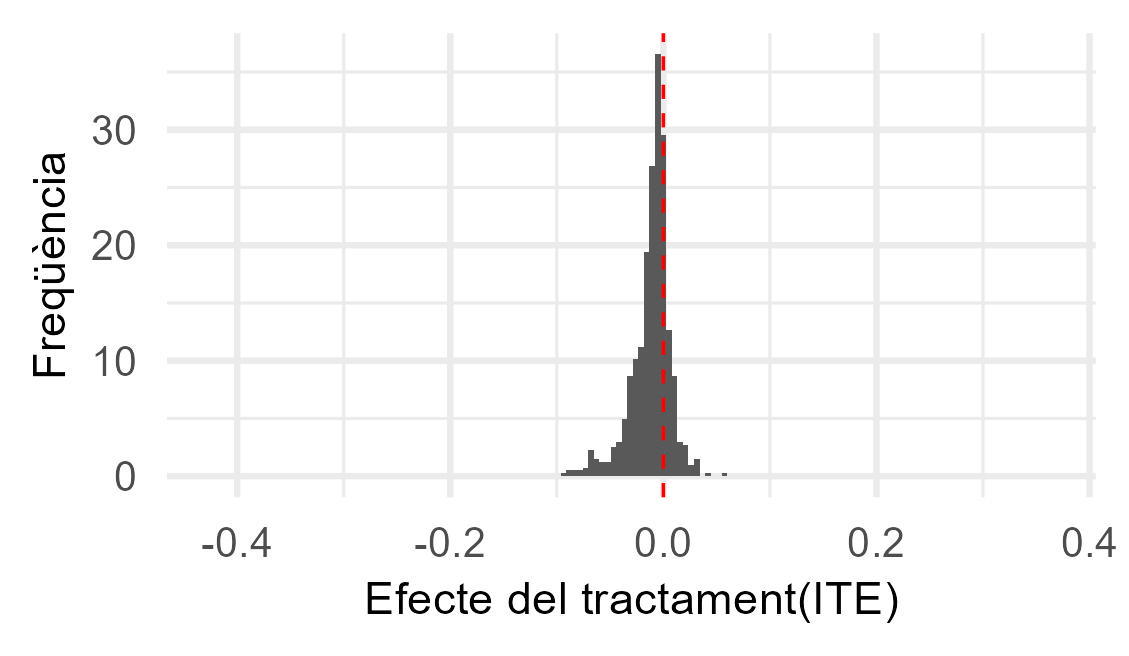
\includegraphics[width=0.3\textwidth]{imgs/histogrames/hist(PE)S_tract2.jpg} &
        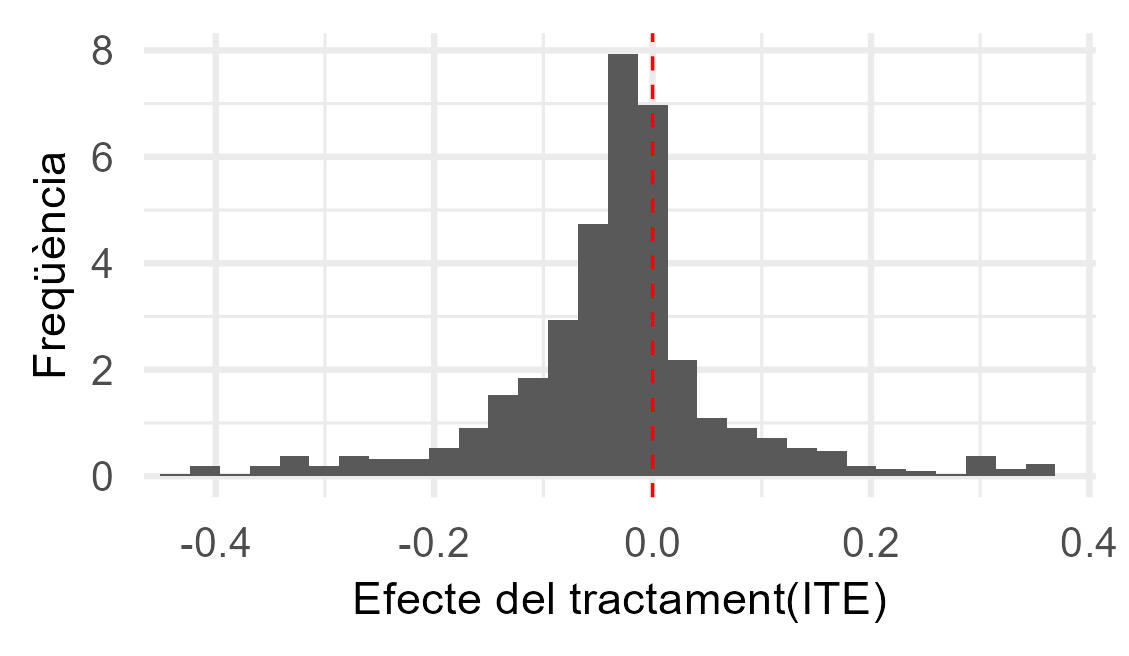
\includegraphics[width=0.3\textwidth]{imgs/histogrames/hist(PE)T_tract2.jpg} &
        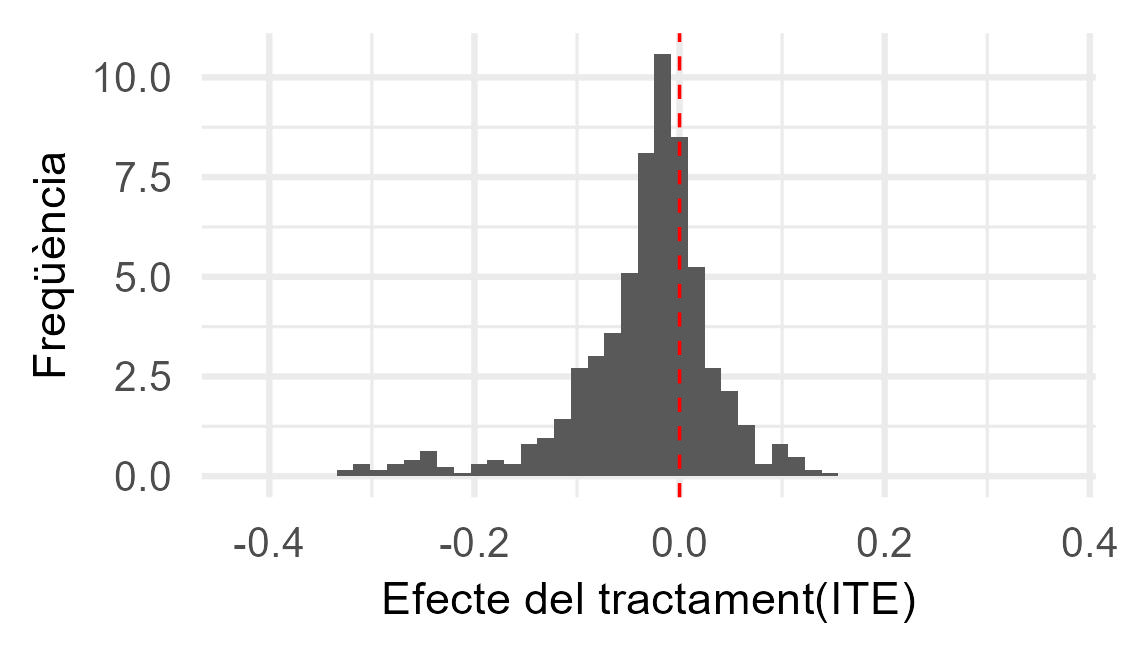
\includegraphics[width=0.3\textwidth]{imgs/histogrames/hist(PE)X_tract2.jpg} \\
        \end{tabular}
        \caption{\footnotesize Comparació visual dels ITEs i ATE estimats amb S-, T- i X-learner per la variable resposta \textit{preeclàmpsia durant l’embaràs}}
        \label{tab:histITE_PE2}
    \end{table}

    En aquesta variable, les distribucions dels ITEs es mostren molt més centrades al voltant del valor zero en comparació amb altres outcomes, tot i continuar indicant un efecte beneficiós del tractament. Això es reflecteix clarament en l’ATE estimat amb l’X-learner, que se situa en -0.34, així com en l’elevat pic central i la menor dispersió, indicativa d’una variabilitat reduïda.
 
    
%histogrames reducció d'estrès    
    \begin{table}[H]
        \centering
        \begin{tabular}{ccc}
        \multicolumn{3}{c}{Histograma de l'ITE amb \textbf{reducció estrès}} \\
        \small \textbf{S-learner} & \small \textbf{T-learner} & \small \textbf{X-learner} \\
        \footnotesize ATE = -0.011 & \footnotesize ATE = -0.030 & \footnotesize ATE = -0.035 \\
        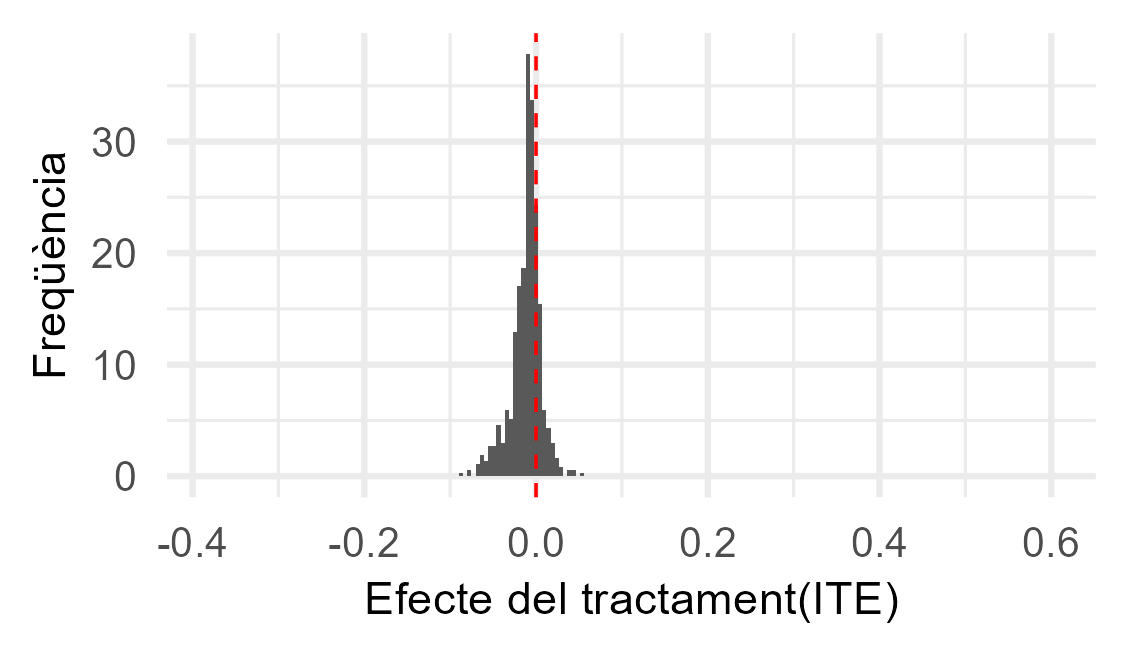
\includegraphics[width=0.3\textwidth]{imgs/histogrames/hist(PE)S_tract3.jpg} &
        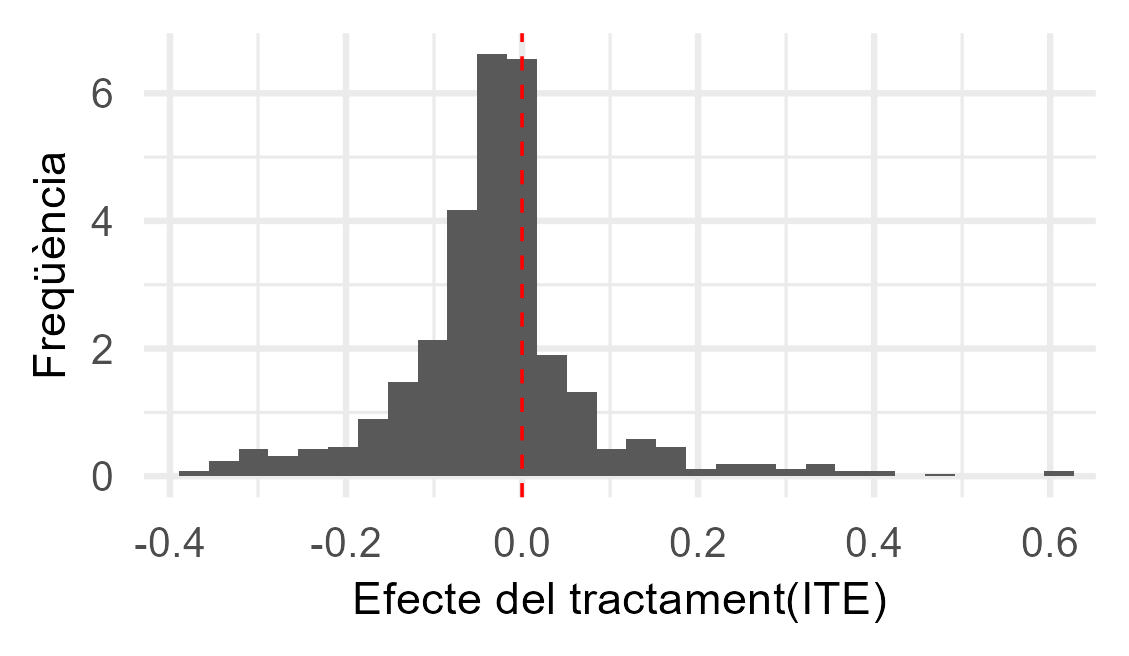
\includegraphics[width=0.3\textwidth]{imgs/histogrames/hist(PE)T_tract3.jpg} &
        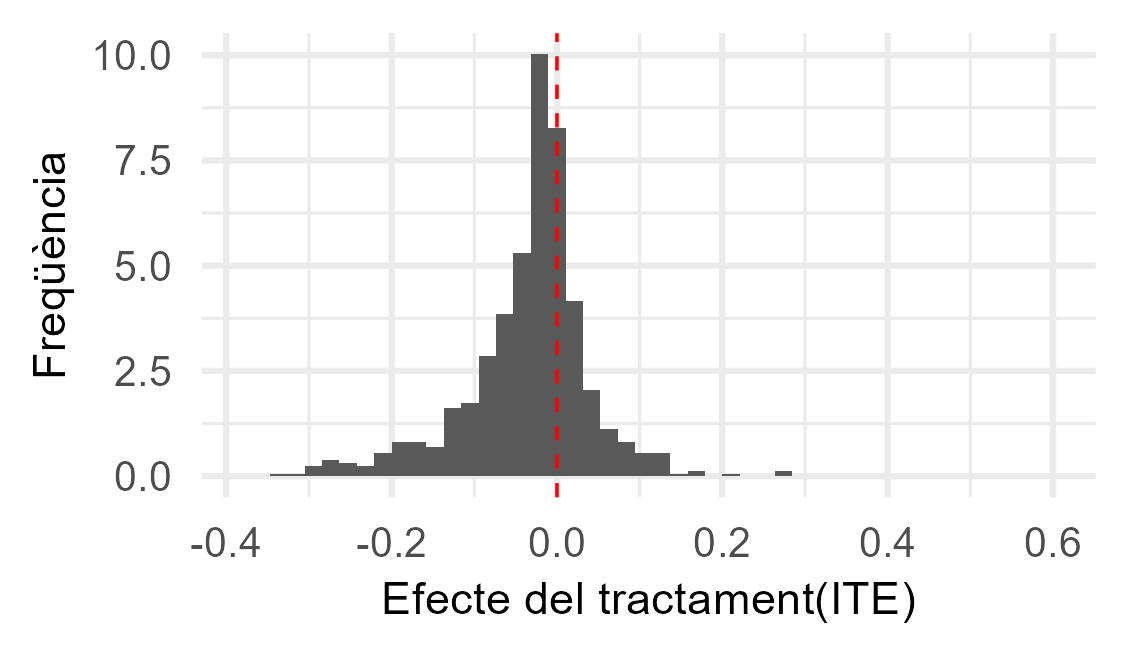
\includegraphics[width=0.3\textwidth]{imgs/histogrames/hist(PE)X_tract3.jpg} \\
        \end{tabular}
        \caption{\footnotesize Comparació visual dels ITEs i ATE estimats amb S-, T- i X-learner per la variable resposta \textit{preeclàmpsia durant l’embaràs}}
        \label{tab:histITE_PE3}
    \end{table}
    
    Pel que fa al tractament amb reducció d'estrès, el comportament és molt similar al de dieta mediterrània. Aquí la disminució mitjana de la probabilitat de desenvolupar preeclàmpsia durant l’embaràs és del 3.5\%. I la distribució dels ITEs torna a mostrar un pic molt pronunciat al voltant de la mitjana i una variabilitat baixa, la qual cosa suggereix una kurtosi positiva, amb la major part de l’efecte concentrat entorn del valor central.
    
%taula coeficients
    \begin{table}[H]
        \centering
        \captionsetup{font=small}        
        \caption{Coeficients estimats i intervals de confiança model lineal per CATE de PE}
        \label{tab:coef_PE}
        \centering
        \scriptsize
        \begin{tabular}[t]{p{4cm} c @{\hspace{1cm}} c}
        \toprule
        Variable & Tractament  & Tractament \\
         & Dieta mediterrània & Reducció estrès \\
        \midrule
        (Intercept) & \textbf{0.25 (0.16; 0.34)} & -0.07 (-0.17; 0.03)\\
        Edat & 0.00 (-0.00; 0.00) & \textbf{0.00 (0.00; 0.00)}\\
        Talla & \textbf{-0.00 (-0.00; -0.00)} & 0.00 (-0.00; 0.00)\\
        IMC pregestacional & \textbf{-0.00 (-0.00; -0.00)} & \textbf{-0.00 (-0.00; -0.00)}\\
        Fumadora & \textbf{-0.04 (-0.07; -0.01)} & \textbf{-0.05 (-0.07; -0.02)}\\
        \addlinespace
        Antecedents SGA & -0.01 (-0.02; 0.00) & \textbf{0.02 (0.01; 0.03)}\\
        HTA crònica & \textbf{-0.23 (-0.24; -0.21)} & \textbf{-0.21 (-0.23; -0.20)}\\
        Diabetis gestacional & \textbf{0.07 (0.06; 0.09)} & \textbf{0.03 (0.01; 0.05)}\\
        Nefropatia & -0.02 (-0.04; 0.00) & \textbf{0.12 (0.09; 0.14)}\\
        Malaltia autoimmune & \textbf{-0.02 (-0.03; -0.01)} & 0.00 (-0.01; 0.01)\\
        \addlinespace
        Doppler patològic & 0.01 (-0.00; 0.03) & 0.01 (-0.00; 0.03)\\
        Risc PE & \textbf{-0.01 (-0.02; -0.00)} & \textbf{0.02 (0.01; 0.03)}\\
        PAPP-A patològic & \textbf{0.02 (0.01; 0.04)} & -0.01 (-0.03; 0.00)\\
        Metrorràgia & \textbf{-0.02 (-0.03; -0.00)} & \textbf{-0.08 (-0.09; -0.06)}\\
        Criteris SGA & \textbf{-0.02 (-0.03; -0.01)} & \textbf{-0.02 (-0.03; -0.01)}\\
        \addlinespace
        Fecundació assistida & \textbf{-0.03 (-0.04; -0.02)} & \textbf{-0.01 (-0.02; -0.00)}\\
        Nul·liparitat & \textbf{-0.01 (-0.02; -0.00)} & \textbf{-0.01 (-0.02; -0.01)}\\
        \bottomrule
        \multicolumn{3}{l}{\rule{0pt}{1em}*coef (IC$_{95\%}$); \textit{Amb negreta les variables significatives amb $\alpha=0.05$}}
        \end{tabular}
    \end{table}

    A partir dels coeficients estimats als models de la taula \ref{tab:coef_PE}, s’observa que determinades variables maternes contribueixen a incrementar l’efecte beneficiós dels tractaments sobre la reducció del risc de preeclàmpsia. En concret, el \textit{BMI pregestacional}, el fet de ser \textit{fumadora}, la presència de \textit{metrorràgia}, el compliment de \textit{criteris clínics menors de risc d’SGA}, que l’embaràs hagi estat \textit{concebut mitjançant TRA}, la \textit{nul·liparitat} i, de manera destacada, la \textit{hipertensió arterial crònica}, es relacionen amb una major efectivitat del tractament en \textbf{ambdós grups}.\par
    Però la \textit{diabetis durant l’embaràs} genera heterogeneïtat en sentit contrari, reduint l’efecte positiu del tractament en el subgrup de mares que la presenten.\par
    Pel que fa al tractament de \textbf{dieta mediterrània}, més enllà de les variables compartides, es detecta una resposta menys favorable en mares amb \textit{valors patològics de la proteïna PAPP-A}. Mentre que una \textit{talla materna} més elevada s’associa a una millora més marcada de l’efecte del tractament.\par
    En el cas de la \textbf{reducció d'estrès}, s’observa una reducció de l’efecte en mares de més \textit{edat}, amb \textit{antecedents de nadons amb SGA} o amb diagnòstic de \textit{nefropatia}. Aquestes característiques podrien estar modulant negativament la resposta al tractament dins d’aquests subgrups.
    

    


    \subsection{Preeclàmpsia precoç}\label{subsec:PEearly}

    Una altra de les variables resposta analitzades és la preeclàmpsia precoç, entesa com aquella que es manifesta abans de les 32 setmanes de gestació. Aquesta condició és especialment rellevant, ja que, com s'ha explicat, s’associa sovint a complicacions per la mare i pel fetus, i pot tenir un impacte directe en el creixement fetal i en el desenllaç perinatal.\par
    Cal destacar que es tracta d’una característica poc freqüent en la mostra, ja que només es va observar en un 0,5\% dels casos (6 participants). Aquesta baixa incidència implica que les conclusions que se’n poden extreure manquen de significança estadística i han de ser interpretades amb precaució. Tanmateix, tot i la poca robustesa dels resultats, és interessant analitzar com es comporten els diferents meta-learners en aquest cas.
    
%histogrames amb Dieta mediterrània    
    \begin{table}[H]
        \centering
        \begin{tabular}{ccc}
        \multicolumn{3}{c}{Histograma de l'ITE amb \textbf{dieta mediterrània}} \\
        \small \textbf{S-learner} & \small \textbf{T-learner} & \small \textbf{X-learner} \\
        \footnotesize ATE = 0.001 & \footnotesize ATE = 0.002 & \footnotesize ATE = 0.003 \\
        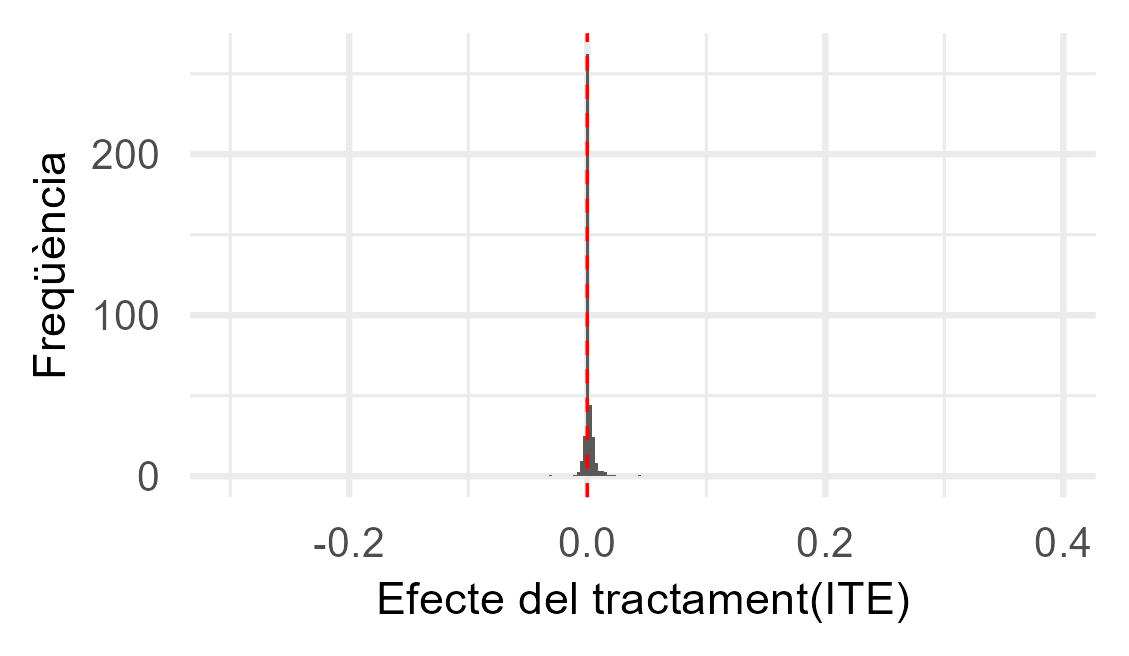
\includegraphics[width=0.3\textwidth]{imgs/histogrames/hist(PEearly)S_tract2.jpg} &
        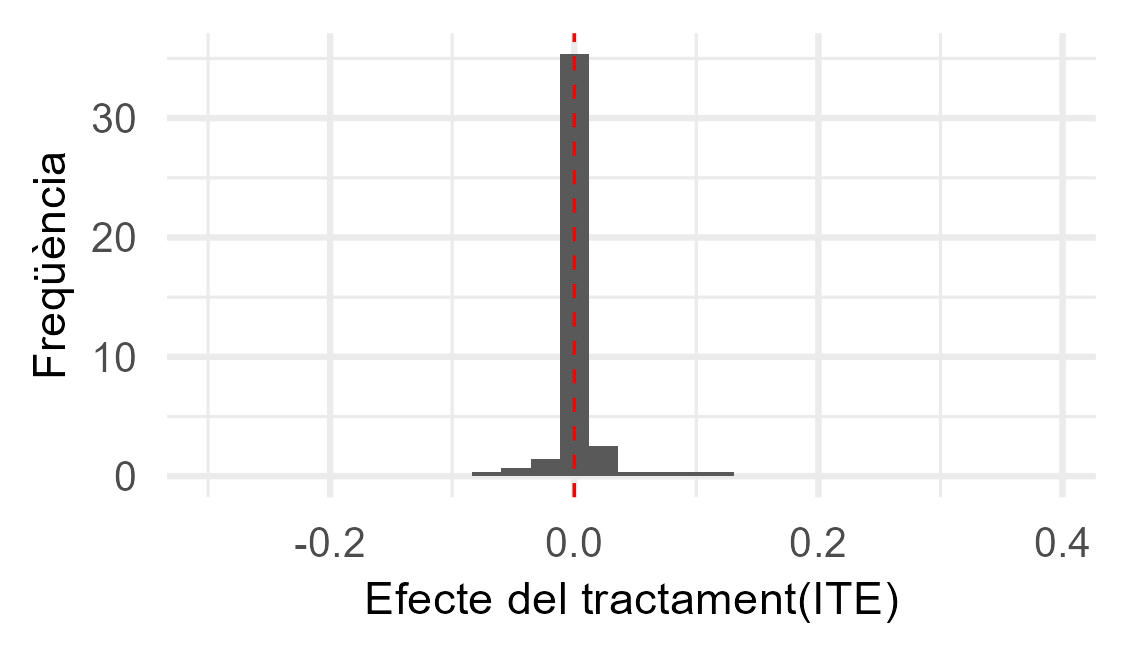
\includegraphics[width=0.3\textwidth]{imgs/histogrames/hist(PEearly)T_tract2.jpg} &
        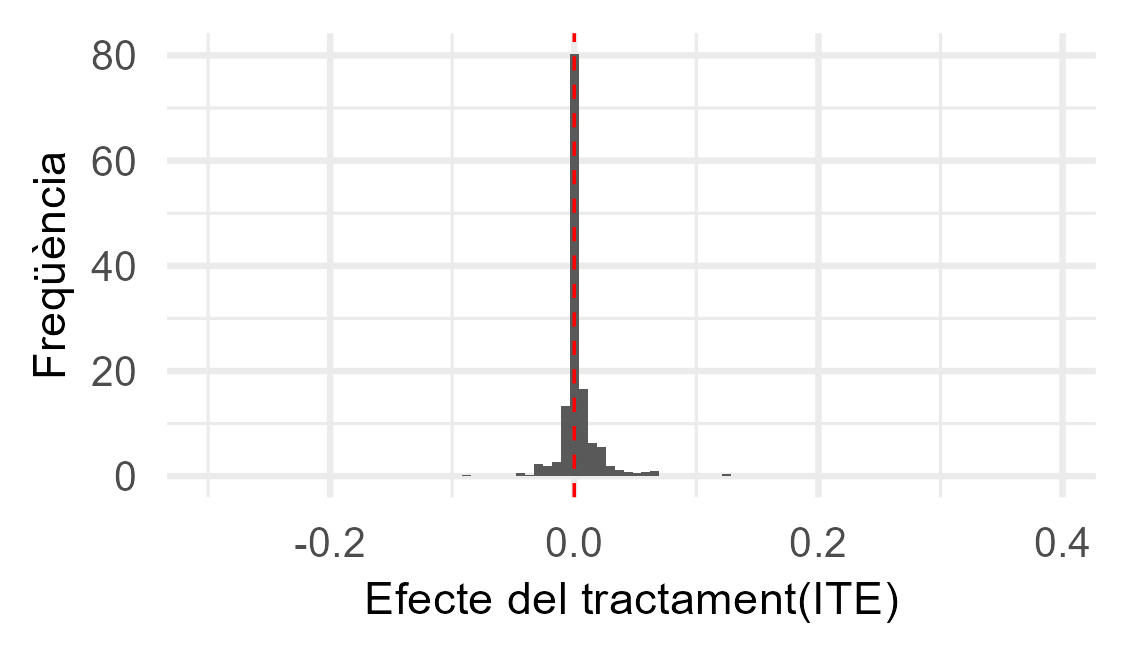
\includegraphics[width=0.3\textwidth]{imgs/histogrames/hist(PEearly)X_tract2.jpg} \\
        \end{tabular}
        \caption{\footnotesize Comparació visual dels ITEs i ATE estimats amb S-, T- i X-learner per la variable resposta \textit{preeclàmpsia precoç}} 
        \label{tab:histITE_PEearly2}
    \end{table}

    Tal com s’ha comentat anteriorment, el nombre de casos amb preeclàmpsia precoç és molt reduït, però força equilibrat entre els tres grups d’intervenció, fet que dona certa credibilitat a l’ATE proper a zero observat pel tractament de reducció de l’estrès. En aquest context, l’S-learner mostra una distribució dels ITEs més que en cap altre outcome i el T-learner continua sent el que més variabilitat presenta, tot i que és considerablement menor que en altres casos.


%histogrames reducció d'estrès
    \begin{table}[H]
        \centering
        \begin{tabular}{ccc}
        \multicolumn{3}{c}{Histograma de l'ITE amb \textbf{reducció estrès}} \\
        \small \textbf{S-learner} & \small \textbf{T-learner} & \small \textbf{X-learner} \\
        \footnotesize ATE = 0.001 & \footnotesize ATE = 0.006 & \footnotesize ATE = 0.005 \\
        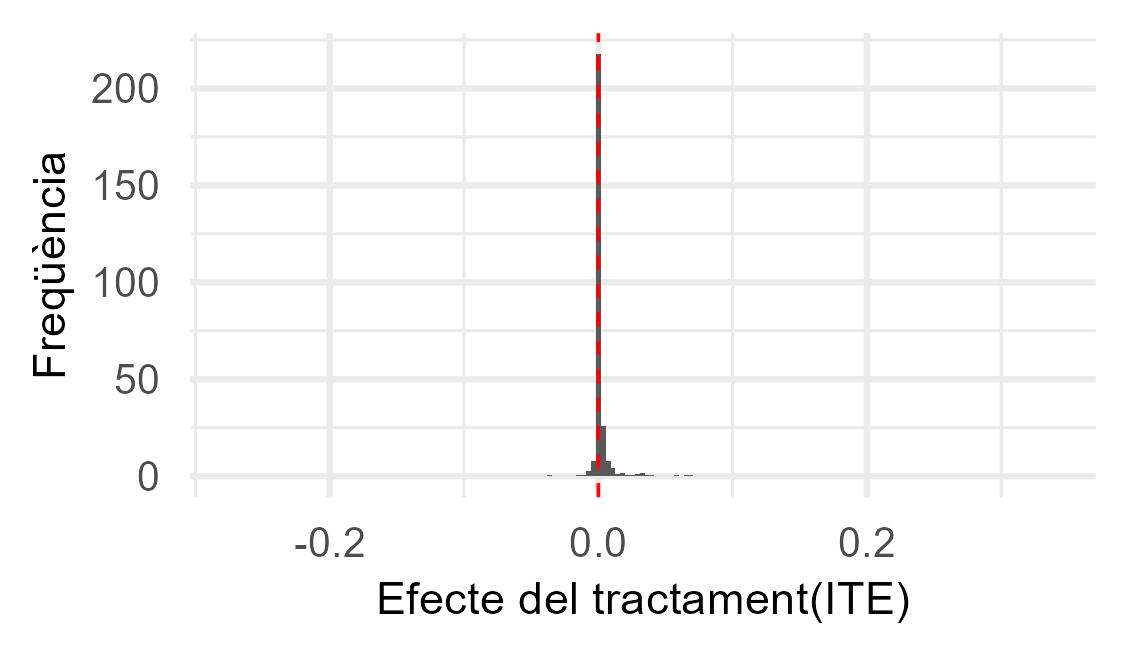
\includegraphics[width=0.3\textwidth]{imgs/histogrames/hist(PEearly)S_tract3.jpg} &
        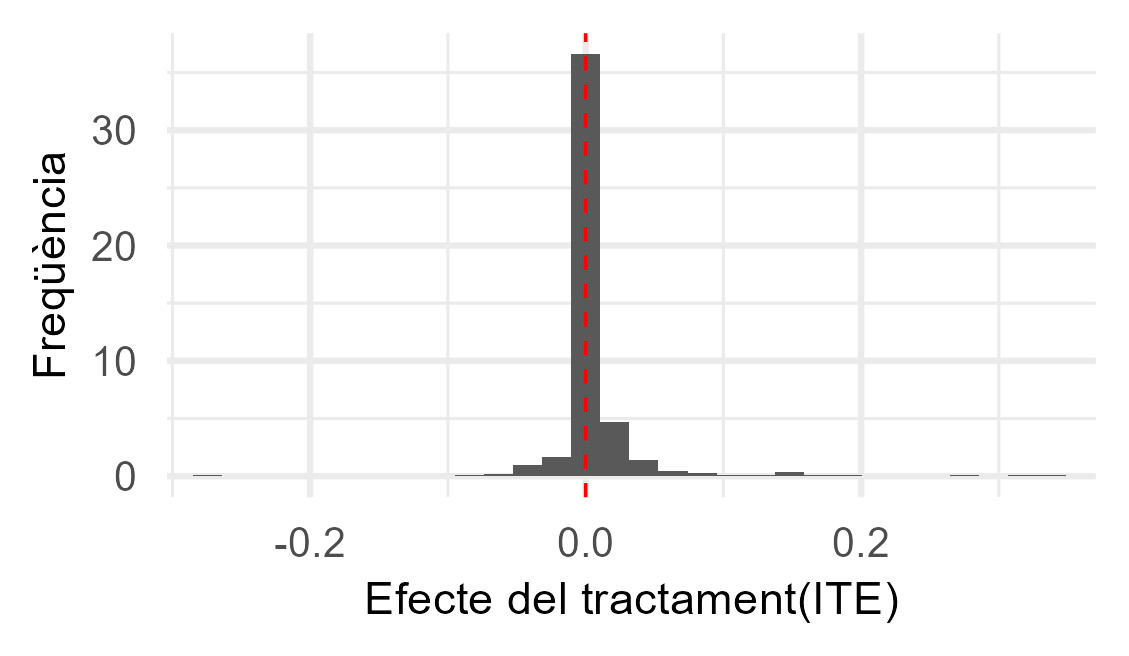
\includegraphics[width=0.3\textwidth]{imgs/histogrames/hist(PEearly)T_tract3.jpg} &
        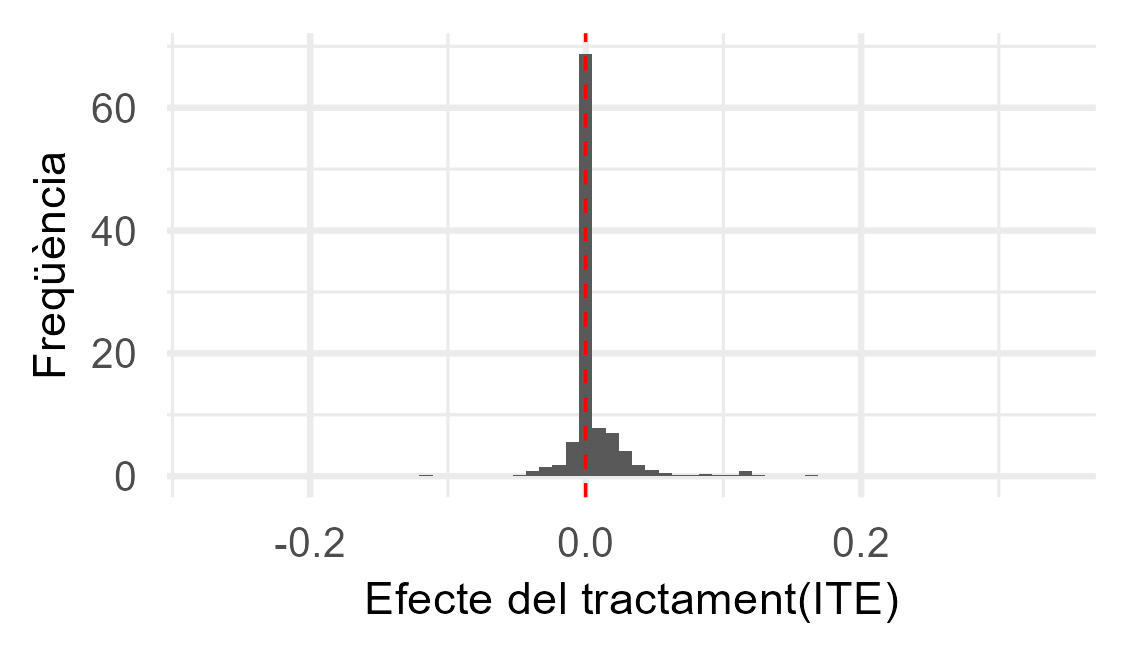
\includegraphics[width=0.3\textwidth]{imgs/histogrames/hist(PEearly)X_tract3.jpg} \\
        \end{tabular}
        \caption{\footnotesize Comparació visual dels ITEs i ATE estimats amb S-, T- i X-learner per la variable resposta \textit{preeclàmpsia precoç}}
        \label{tab:histITE_PEearly3}
    \end{table}
    
    Pel que fa a la reducció d'estrès, la situació és similar a la de dieta mediterrània, amb els ITEs majoritàriament centrats al voltant del valor nul. Però, tant el T-learner com l’X-learner semblen identificar una petita concentració de casos amb efectes positius del tractament, alguns casos on s'incrementa la probabilitat de desenvolupar preeclàmpsia precoç amb el tractament.\par
    Tot i que aquests resultats no poden considerar-se concloents per manca de potència estadística, són indicatius de que el comportament dels meta-learners en contextos amb esdeveniments molt rars no és purament atzarós.\par
    Aquesta manca de robustesa fa que no sigui adequat avaluar els coeficients del model lineal, ja que el nombre molt reduït de casos pot donar lloc a estimacions sense prou validesa estadística com per extreure’n conclusions fiables.



%taula coeficients
    % \begin{table}[H]
    %     \centering
    %     \captionsetup{font=small}
    %     \caption{Coeficients estimats i intervals de confiança model lineal per CATE de PEearly}
    %     \centering
    %     \scriptsize
    %     \begin{tabular}[t]{p{4cm} c @{\hspace{1cm}} c}
    %     \toprule
    %     Variable & Tractament  & Tractament \\
    %      & Dieta mediterrània & Reducció d'estrès \\
    %     \midrule
    %     (Intercept) & \textbf{0.07 (0.05; 0.09)} & -0.01 (-0.03; 0.02)\\
    %     Edat & 0.00 (-0.00; 0.00) & \textbf{0.00 (0.00; 0.00)}\\
    %     Talla & \textbf{-0.00 (-0.00; -0.00)} & \textbf{-0.00 (-0.00; -0.00)}\\
    %     IMC pregestacional & \textbf{0.00 (0.00; 0.00)} & \textbf{0.00 (0.00; 0.00)}\\
    %     Fumadora & 0.01 (-0.00; 0.01) & 0.00 (-0.00; 0.01)\\
    %     \addlinespace
    %     Antecedents SGA & 0.00 (-0.00; 0.00) & \textbf{0.00 (0.00; 0.01)}\\
    %     HTA crònica & -0.00 (-0.00; 0.00) & \textbf{0.05 (0.05; 0.06)}\\
    %     Diabetis gestacional & -0.00 (-0.01; 0.00) & 0.00 (-0.00; 0.01)\\
    %     Nefropatia & 0.00 (-0.00; 0.01) & 0.00 (-0.00; 0.01)\\
    %     Malaltia autoimmune & \textbf{-0.01 (-0.01; -0.01)} & \textbf{-0.01 (-0.01; -0.01)}\\
    %     \addlinespace
    %     Doppler patològic & \textbf{0.03 (0.03; 0.04)} & 0.00 (-0.00; 0.00)\\
    %     Risc PE & 0.00 (-0.00; 0.00) & \textbf{0.01 (0.01; 0.01)}\\
    %     PAPP-A patològic & 0.00 (-0.00; 0.00) & \textbf{0.00 (0.00; 0.01)}\\
    %     Metrorràgia & 0.00 (-0.00; 0.00) & \textbf{-0.00 (-0.01; -0.00)}\\
    %     Criteris SGA & \textbf{0.00 (0.00; 0.01)} & \textbf{0.01 (0.00; 0.01)}\\
    %     \addlinespace
    %     Fecundació assistida & -0.00 (-0.00; 0.00) & \textbf{0.01 (0.01; 0.02)}\\
    %     Nul·liparitat & 0.00 (-0.00; 0.00) & \textbf{0.00 (0.00; 0.01)}\\
    %     \bottomrule
    %     \multicolumn{3}{l}{\rule{0pt}{1em}*\textit{Amb negreta les variables significatives amb $\alpha=0.05$}}
    %     \end{tabular}
    % \end{table}




    
    \subsection{Preeclàmpsia tardana}\label{subsec:PElate}

    La preeclàmpsia tardana es defineix com aquella que es manifesta a partir de la setmana 32 de gestació. Tot i que clínicament pot ser menys greu que la preeclàmpsia precoç, continua sent un factor de risc important per a la salut materna i fetal, especialment si no es detecta i gestiona adequadament.
    
%histogrames amb dieta mediterrània    
    \begin{table}[H]
        \centering
        \begin{tabular}{ccc}
        \multicolumn{3}{c}{Histograma de l'ITE amb \textbf{dieta mediterrània}} \\
        \small \textbf{S-learner} & \small \textbf{T-learner} & \small \textbf{X-learner} \\
        \footnotesize ATE = -0.012 & \footnotesize ATE = -0.038 & \footnotesize ATE = -0.038 \\
        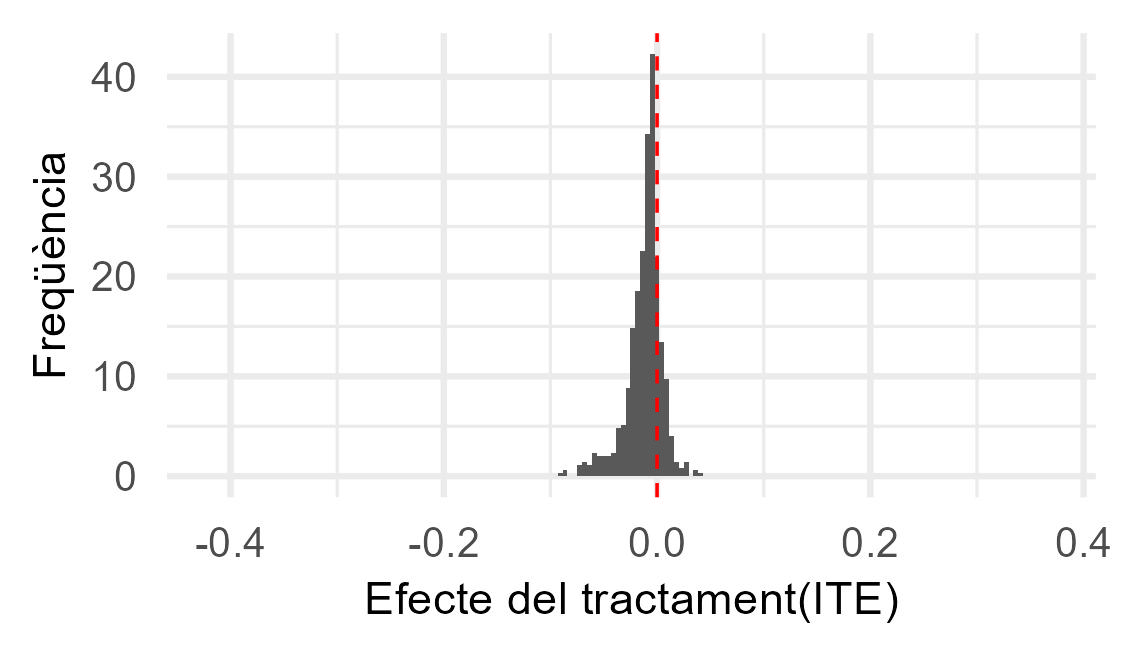
\includegraphics[width=0.3\textwidth]{imgs/histogrames/hist(PElate)S_tract2.jpg} &
        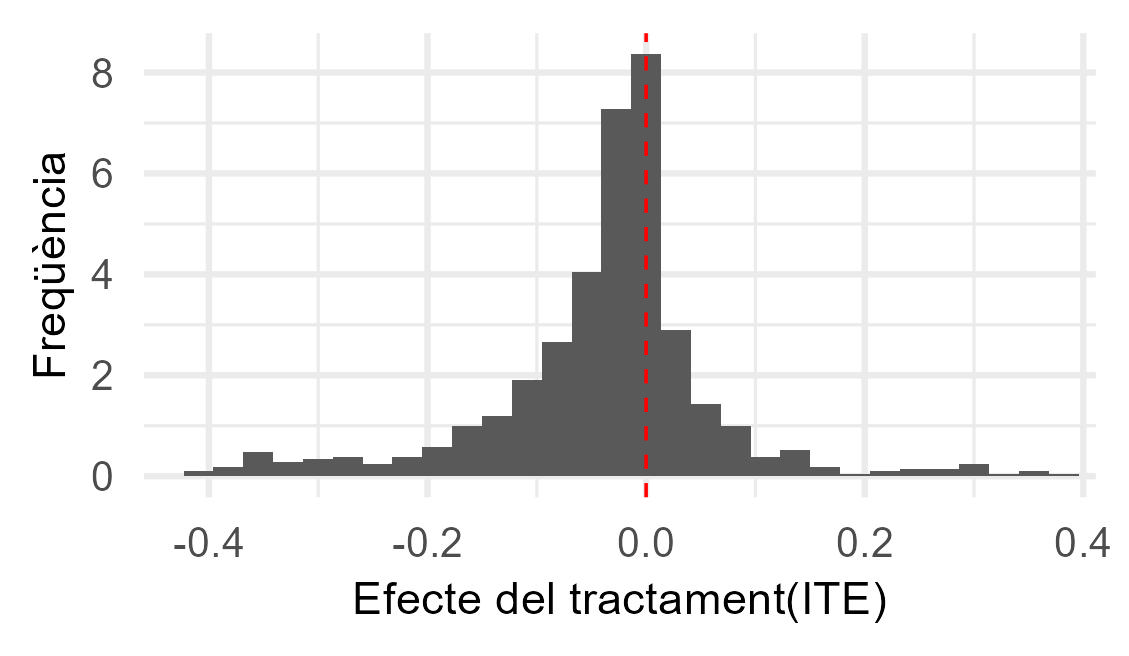
\includegraphics[width=0.3\textwidth]{imgs/histogrames/hist(PElate)T_tract2.jpg} &
        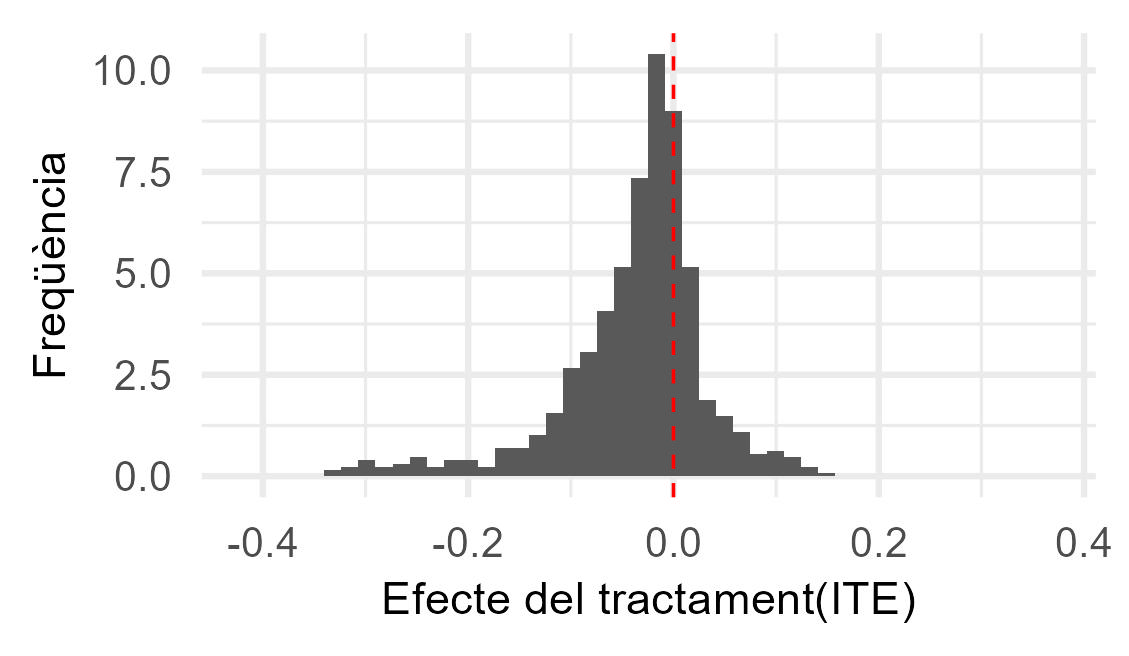
\includegraphics[width=0.3\textwidth]{imgs/histogrames/hist(PElate)X_tract2.jpg} \\
        \end{tabular}
        \caption{\footnotesize Comparació visual dels ITEs i ATE estimats amb S-, T- i X-learner per la variable resposta \textit{preeclàmpsia tardana}}
        \label{tab:histITE_PElate2}
    \end{table}

    En aquest cas, es torna a observar un augment en la variabilitat de les estimacions dels meta-learners i que es mantenen els patrons generals. L’S-learner continua produint una distribució molt centrada al voltant de zero, amb una variància molt reduïda. El T-learner mostra, com és habitual, la distribució més àmplia i dispersa, mentre que l’X-learner adopta una forma similar a la del T-learner però amb una concentració més clara al voltant del valor mitjà. Pel que fa a l’ATE, tant el T-learner com l’X-learner coincideixen en una estimació de -0.038, la qual cosa indicaria que el tractament de dieta mediterrània redueix de mitjana un 3,8\% la probabilitat de desenvolupar preeclàmpsia tardana.

%histogrames reducció d'estrès 
    \begin{table}[H]
        \centering
        \begin{tabular}{ccc}
        \multicolumn{3}{c}{Histograma de l'ITE amb \textbf{reducció estrès}} \\
        \small \textbf{S-learner} & \small \textbf{T-learner} & \small \textbf{X-learner} \\
        \footnotesize ATE = -0.014 & \footnotesize ATE = -0.039 & \footnotesize ATE = -0.038 \\
        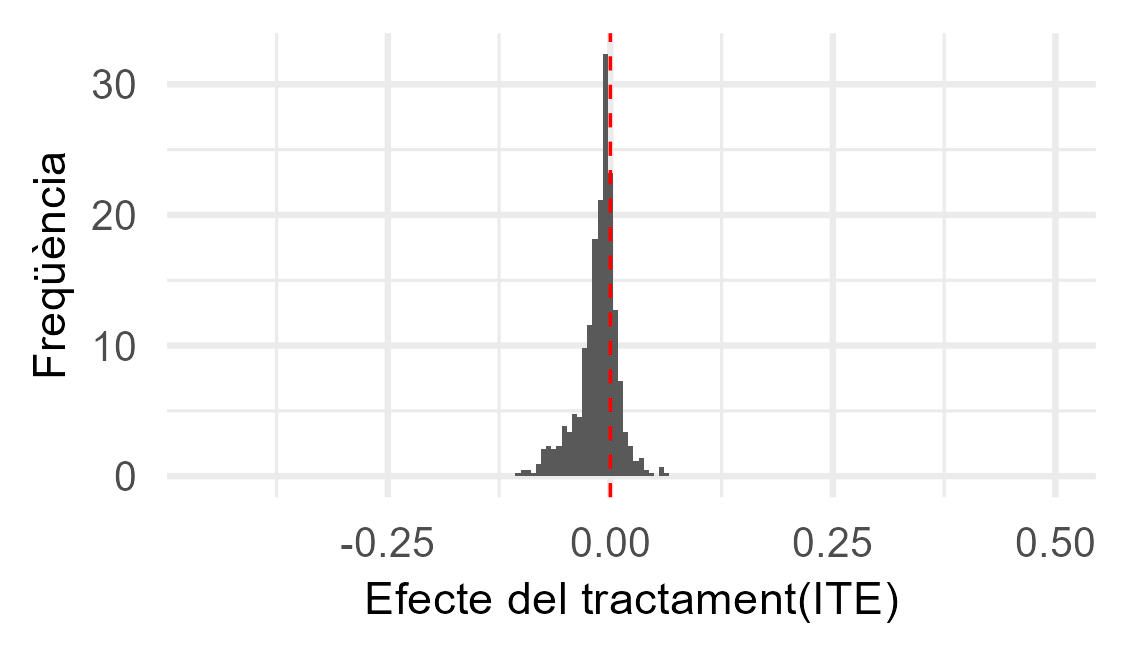
\includegraphics[width=0.3\textwidth]{imgs/histogrames/hist(PElate)S_tract3.jpg} &
        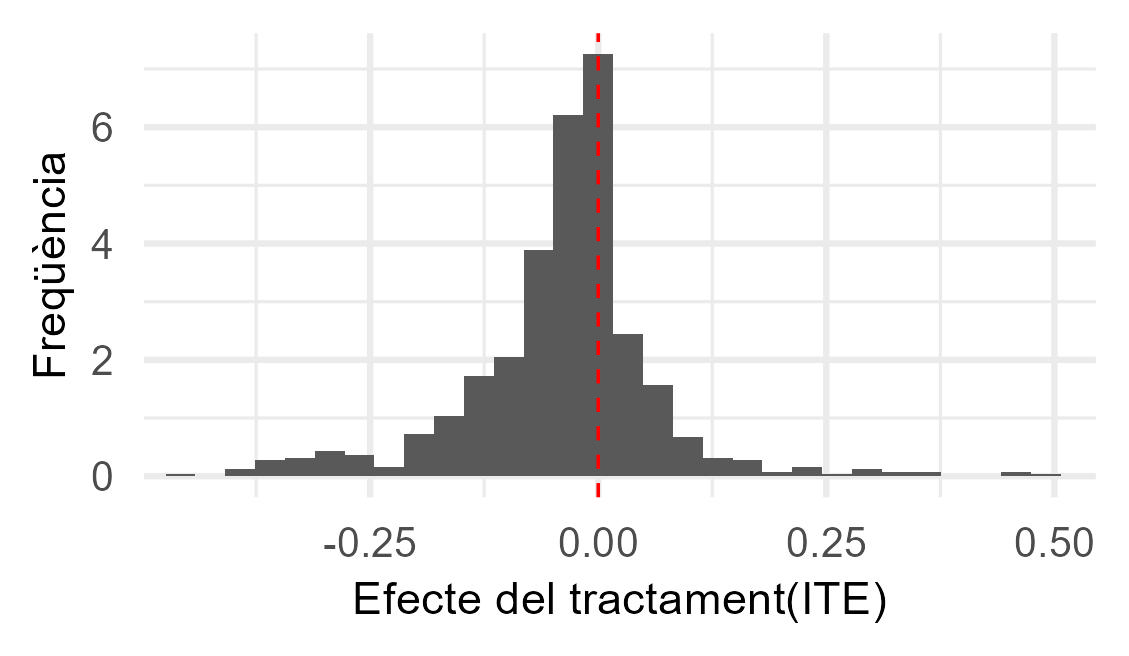
\includegraphics[width=0.3\textwidth]{imgs/histogrames/hist(PElate)T_tract3.jpg} &
        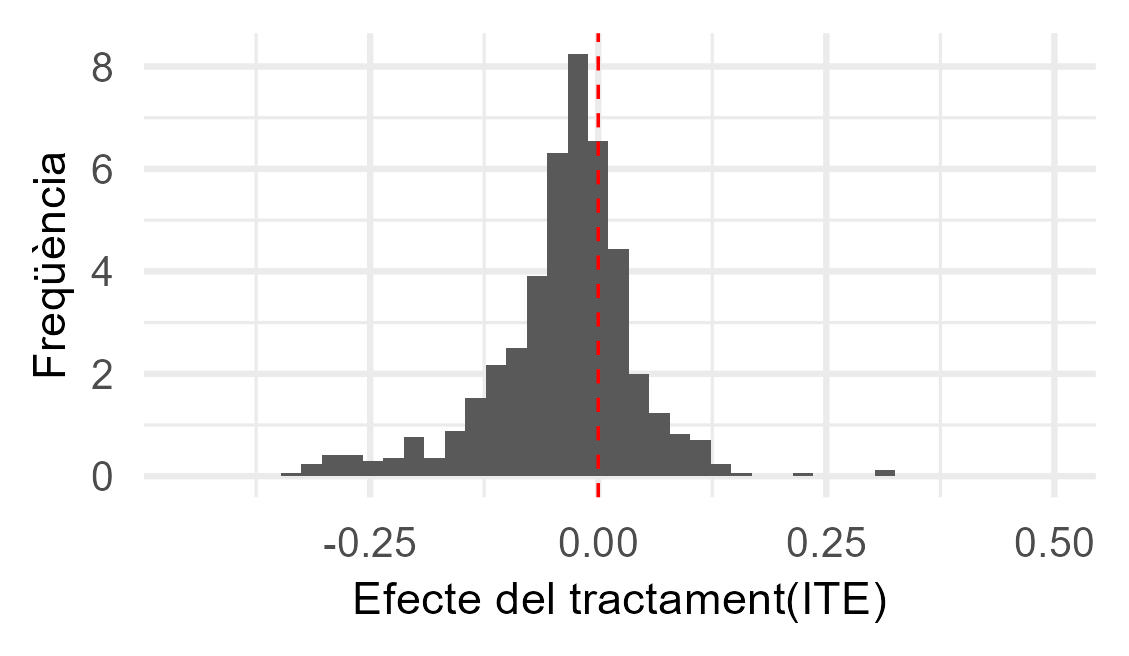
\includegraphics[width=0.3\textwidth]{imgs/histogrames/hist(PElate)X_tract3.jpg} \\
        \end{tabular}
        \caption{\footnotesize Comparació visual dels ITEs i ATE estimats amb S-, T- i X-learner per la variable resposta \textit{preeclàmpsia tardana}}
        \label{tab:histITE_PElate3}
    \end{table}

    La distribució dels efectes individuals associats a la reducció d'estrès presenta un comportament pràcticament idèntic al altre tractament. I l’ATE estimat és també molt proper -0.038 amb l'X-learner. Un aspecte destacable és la presència d’una cua més pesant cap a la banda negativa en les distribucions del T-learner i de l’X-learner, fet que podria suggerir l’existència d’un subgrup de pacients que es beneficia especialment d’aquest tractament. Una heterogeneïtat que explorarem a continuació.
    
%taula coefcients
    \begin{table}[H]
        \centering
        \captionsetup{font=small}
        \caption{Coeficients estimats i intervals de confiança model lineal per CATE de PE tardana}
        \label{tab:coef_PEtard}
        \centering
        \scriptsize
        \begin{tabular}[t]{p{4cm} c @{\hspace{1cm}} c}
        \toprule
        Variable & Tractament  & Tractament \\
         & Dieta mediterrània & Reducció estrès \\
        \midrule
        (Intercept) & \textbf{0.13 (0.04; 0.22)} & -0.08 (-0.17; 0.02)\\
        Edat & \textbf{0.00 (0.00; 0.00)} & \textbf{0.00 (0.00; 0.00)}\\
        Talla & \textbf{-0.00 (-0.00; -0.00)} & \textbf{0.00 (0.00; 0.00)}\\
        IMC pregestacional & \textbf{-0.00 (-0.00; -0.00)} & \textbf{-0.00 (-0.00; -0.00)}\\
        Fumadora & \textbf{-0.04 (-0.07; -0.01)} & \textbf{-0.05 (-0.07; -0.02)}\\
        \addlinespace
        Antecedents SGA & -0.01 (-0.02; 0.00) & \textbf{0.03 (0.02; 0.04)}\\
        HTA crònica & \textbf{-0.22 (-0.24; -0.20)} & \textbf{-0.23 (-0.25; -0.22)}\\
        Diabetis gestacional & \textbf{0.08 (0.06; 0.09)} & \textbf{0.03 (0.02; 0.05)}\\
        Nefropatia & -0.02 (-0.04; 0.00) & \textbf{0.13 (0.11; 0.15)}\\
        Malaltia autoimmune & \textbf{-0.02 (-0.02; -0.01)} & \textbf{0.01 (0.00; 0.02)}\\
        \addlinespace
        Doppler patològic & \textbf{-0.02 (-0.03; -0.00)} & 0.01 (-0.00; 0.03)\\
        Risc PE & \textbf{-0.02 (-0.02; -0.01)} & 0.01 (-0.00; 0.01)\\
        PAPP-A patològic & \textbf{0.02 (0.01; 0.03)} & -0.01 (-0.03; 0.00)\\
        Metrorràgia & \textbf{-0.02 (-0.03; -0.00)} & \textbf{-0.06 (-0.07; -0.04)}\\
        Criteris SGA & \textbf{-0.03 (-0.04; -0.02)} & \textbf{-0.03 (-0.04; -0.02)}\\
        \addlinespace
        Fecundació assistida & \textbf{-0.03 (-0.04; -0.02)} & \textbf{-0.03 (-0.03; -0.02)}\\
        Nul·liparitat & \textbf{-0.01 (-0.02; -0.00)} & \textbf{-0.02 (-0.03; -0.01)}\\
        \bottomrule
        \multicolumn{3}{l}{\rule{0pt}{1em}*coef (IC$_{95\%}$); \textit{Amb negreta les variables significatives amb $\alpha=0.05$}}
        \end{tabular}
    \end{table}

    Analitzant els coeficients de la taula \ref{tab:coef_PEtard}, que recullen els efectes heterogenis del tractament sobre la preeclàmpsia tardana. S’observa que \textbf{tant per al tractament de reducció de l’estrès com per a la reducció d'estrès}, l’efecte és més favorable en dones amb un \textit{IMC pregestacional més elevat}, \textit{fumadores}, \textit{nul·lípares}, amb \textit{metrorràgia}, que compleixen \textit{criteris menors de risc d’SGA} o que han tingut l’\textit{embaràs utilitzant TRA}. A més, les mares amb \textit{hipertensió arterial crònica} són, en ambdós casos, les que es beneficien de manera més clara del tractament.\par
    D’altra banda, l’efecte dels tractaments es redueix en mares amb \textit{edat avançada} o amb \textit{diabetis durant l’embaràs}, fet que suggereix una resposta menys favorable en aquests subgrups.\par
    Pel que fa al tractament de \textbf{dieta mediterrània}, si suma una resposta especialment positiva en dones amb \textit{talla més elevada}, amb \textit{malalties autoimmunitàries}, amb resultats \textit{patològics a l’ecografia Doppler} o amb \textit{risc clínic de preeclàmpsia}.\par
    En canvi, amb el tractament de \textbf{reducció de l'estrès}, aquestes mateixes variables \textit{talla} i \textit{autoimmunitat} presenten efectes en sentit contrari, és a dir, redueixen l’efecte del tractament. En el mateix sentit s’hi afegeixen els \textit{antecedents de SGA} i la \textit{nefropatia}, que també s’associen a una resposta menys efectiva.



    
    \subsection{SGA greu}\label{subsec:severeSGA}

    La variable resposta analitzada en aquesta secció és el SGA greu, definit com el cas en què el pes fetal o neonatal se situa per sota del percentil 3 respecte de la seva edat gestacional. Aquest indicador reflecteix situacions de creixement fetal molt compromès i té una elevada rellevància clínica, ja que s’associa amb un augment del risc de morbiditat i mortalitat perinatal, així com amb complicacions en el desenvolupament posterior del nadó.

%histogrames amb dieta mediterrània
    \begin{table}[H]
        \centering
        \begin{tabular}{ccc}
        \multicolumn{3}{c}{Histograma de l'ITE amb \textbf{dieta mediterrània}} \\
        \small \textbf{S-learner} & \small \textbf{T-learner} & \small \textbf{X-learner} \\
        \footnotesize ATE = -0.018 & \footnotesize ATE = -0.049 & \footnotesize ATE = -0.044 \\
        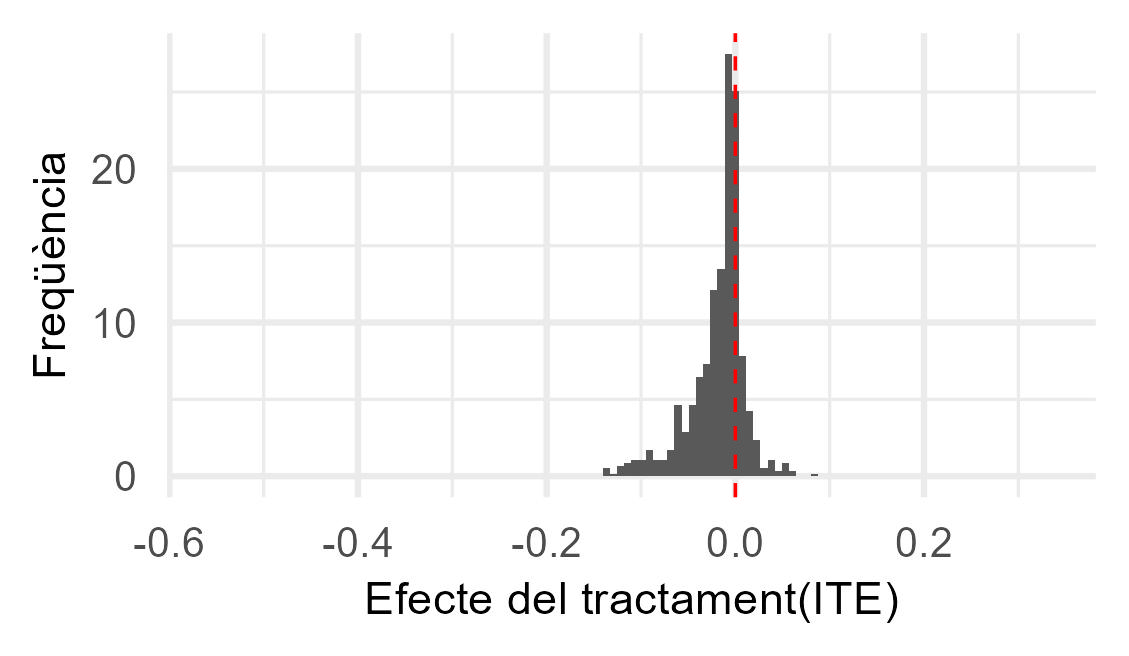
\includegraphics[width=0.3\textwidth]{imgs/histogrames/hist(severeSGA)S_tract2.jpg} &
        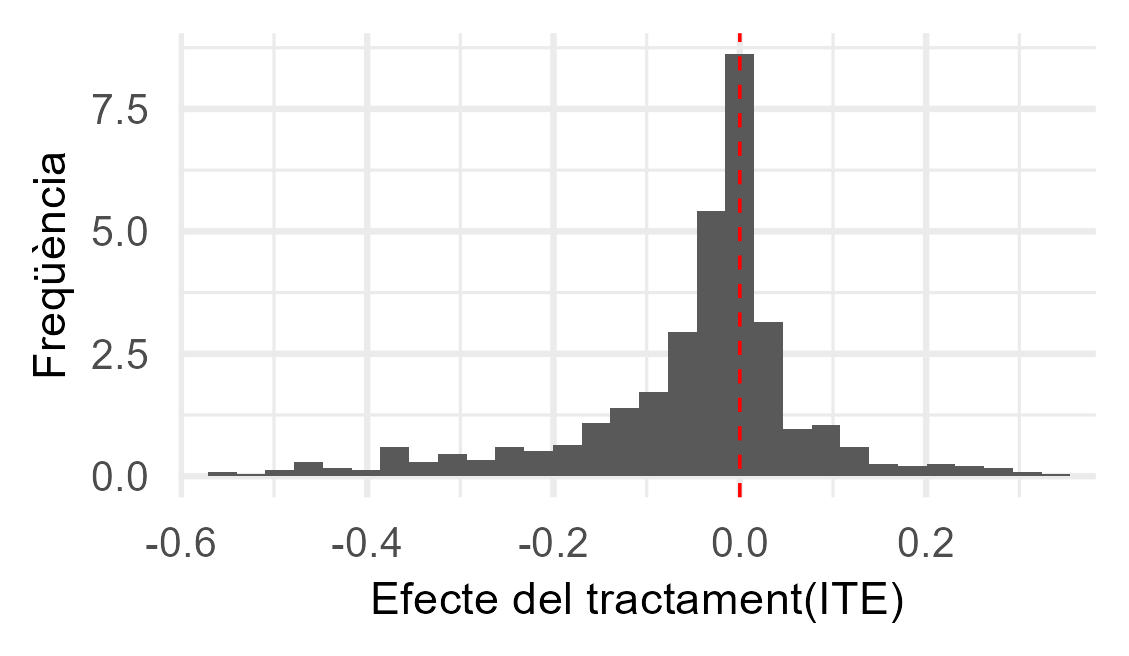
\includegraphics[width=0.3\textwidth]{imgs/histogrames/hist(severeSGA)T_tract2.jpg} &
        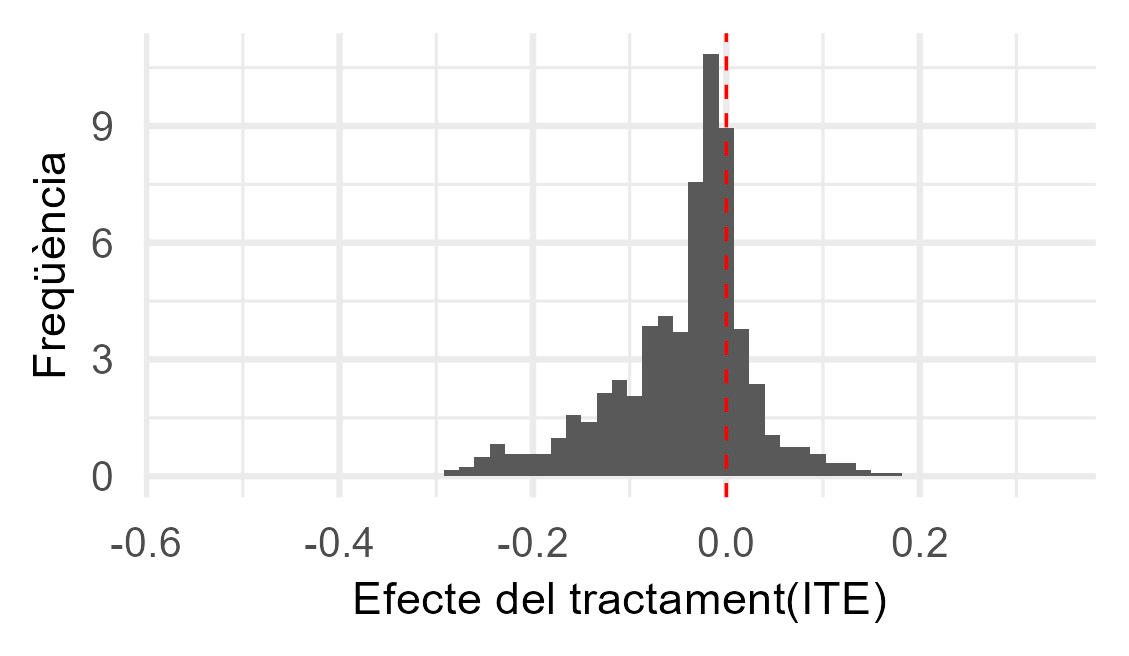
\includegraphics[width=0.3\textwidth]{imgs/histogrames/hist(severeSGA)X_tract2.jpg} \\
        \end{tabular}
        \caption{\footnotesize Comparació visual dels ITEs i ATE estimats amb S-, T- i X-learner per la variable resposta \textit{SGA greu}}
        \label{tab:histITE_severeSGA2}
    \end{table}

    En analitzar l’efecte del tractament de dieta mediterrània sobre l’SGA greu, s’observa que les distribucions dels ITEs estimades pels meta-learners presenten una forma menys propera a la normalitat en comparació amb altres outcomes. El pic al voltant del valor central és molt pronunciat, i les cues són més aplanades, fet que suggereix que els meta-learners, especialment l’S-learner, estan assignant efectes molt similars a la majoria de participants, sense identificar perfils amb respostes clarament diferenciades. L’efecte mitjà del tractament, estimat amb l’X-learner, se situa en -0.044, indicant que, de mitjana, el tractament redueix la probabilitat de SGA greu.

%histogrames amb Reducció d'estrès
    \begin{table}[H]
        \centering
        \begin{tabular}{ccc}
        \multicolumn{3}{c}{Histograma de l'ITE amb \textbf{reducció estrès}} \\
        \small \textbf{S-learner} & \small \textbf{T-learner} & \small \textbf{X-learner} \\
        \footnotesize ATE = -0.019 & \footnotesize ATE = -0.053 & \footnotesize ATE = -0.052 \\
        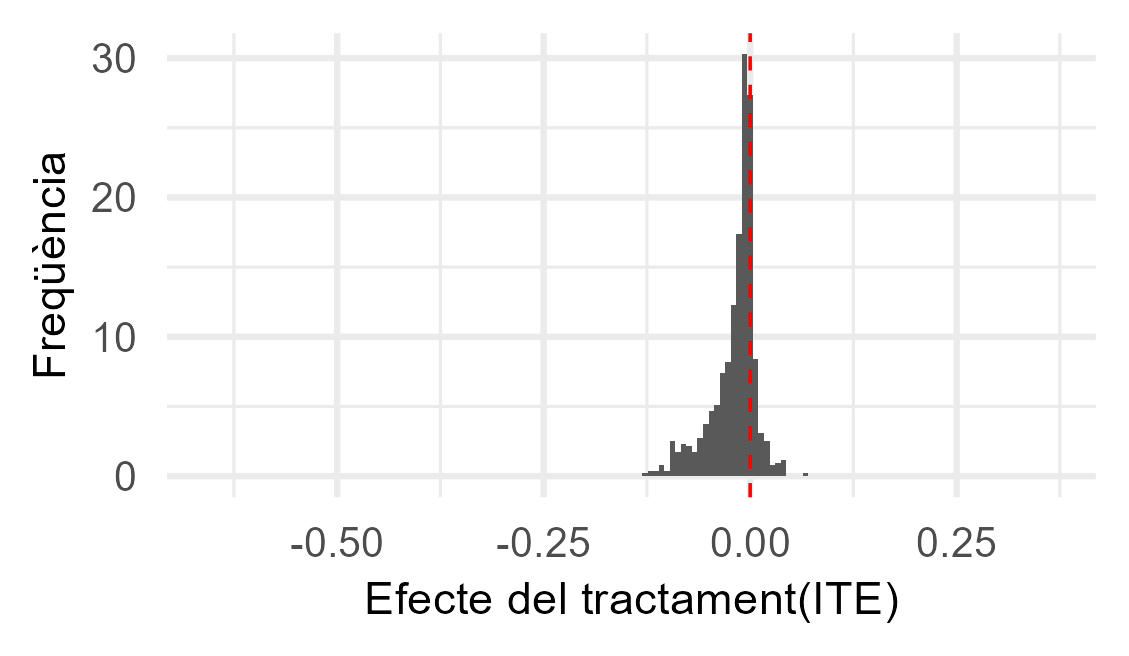
\includegraphics[width=0.3\textwidth]{imgs/histogrames/hist(severeSGA)S_tract3.jpg} &
        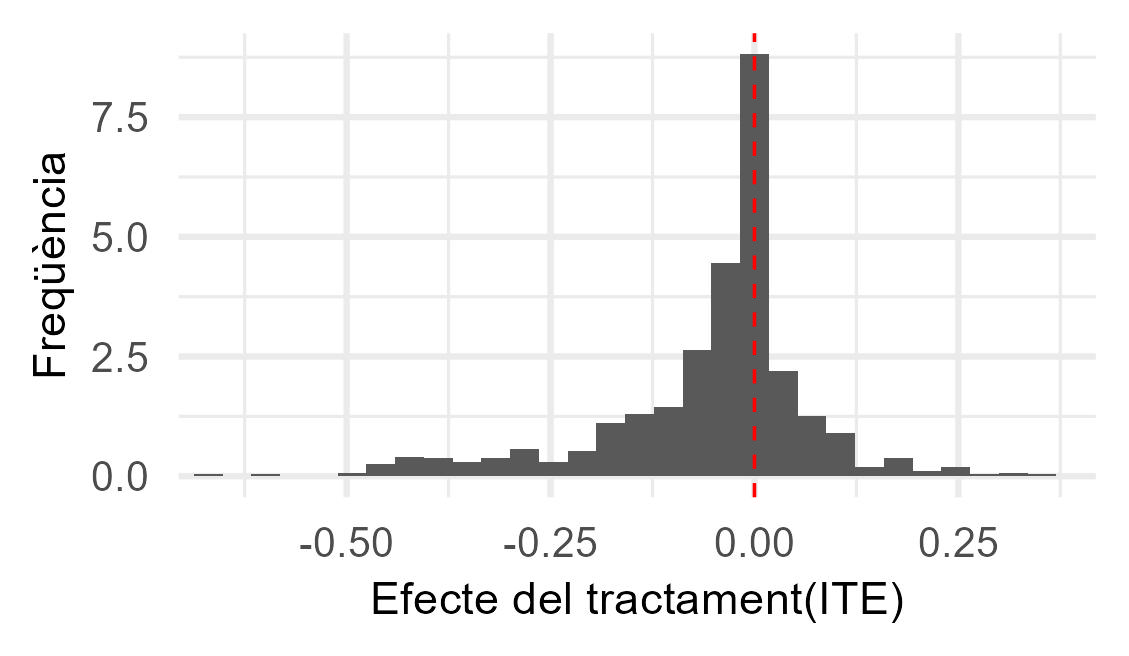
\includegraphics[width=0.3\textwidth]{imgs/histogrames/hist(severeSGA)T_tract3.jpg} &
        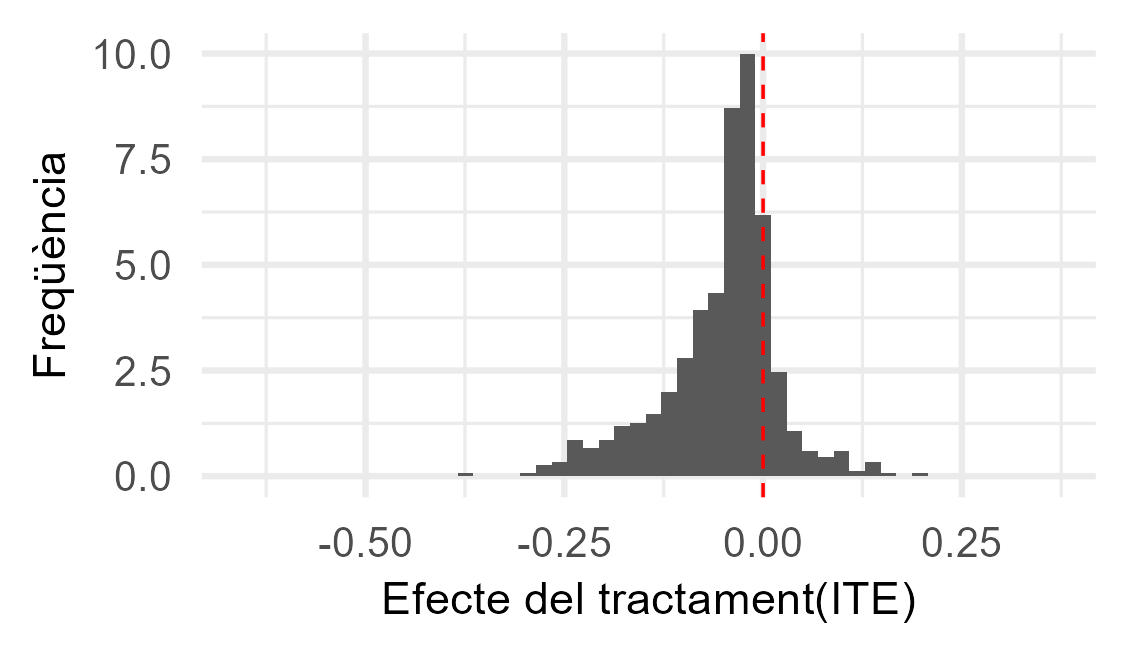
\includegraphics[width=0.3\textwidth]{imgs/histogrames/hist(severeSGA)X_tract3.jpg} \\
        \end{tabular}
        \caption{\footnotesize Comparació visual dels ITEs i ATE estimats amb S-, T- i X-learner per la variable resposta \textit{SGA greu}}
        \label{tab:histITE_severeSGA3}
    \end{table}

    En el cas de la reducció d'estrès, les distribucions dels ITEs són molt similars, però amb cues notablement més pesants cap a la banda negativa, especialment evidents en el T-learner i l’X-learner. Aquesta forma indica que, tot i que la majoria d’individus tenen un efecte proper a zero, hi ha un conjunt de casos amb efectes clarament més beneficiosos (ITE més negatius). Aquest comportament suggereix la presència de subgrups de pacients amb una resposta molt favorable al tractament. L’ATE estimat amb l’X-learner és de -0.052, fet que representa una reducció mitjana del 5.2\% en el risc de SGA greu.


%taula coeficients
    \begin{table}[H]
        \centering
        \captionsetup{font=small}
        \caption{Coeficients estimats i intervals de confiança model lineal per CATE de SGA greu}
        \label{tab:coef_SGAgreu}
        \centering
        \scriptsize
        \begin{tabular}[t]{p{4cm} c @{\hspace{1cm}} c}
        \toprule
        Variable & Tractament  & Tractament \\
         & Dieta mediterrània & Reducció estrès \\
        \midrule
        (Intercept) & -0.08 (-0.18; 0.02) & \textbf{-0.44 (-0.55; -0.33)}\\
        Edat & \textbf{-0.00 (-0.00; -0.00)} & -0.00 (-0.00; 0.00)\\
        Talla & 0.00 (-0.00; 0.00) & \textbf{0.00 (0.00; 0.00)}\\
        IMC pregestacional & \textbf{0.00 (0.00; 0.00)} & -0.00 (-0.00; 0.00)\\
        Fumadora & \textbf{-0.04 (-0.07; -0.01)} & \textbf{-0.06 (-0.09; -0.03)}\\
        \addlinespace
        Antecedents SGA & \textbf{0.02 (0.01; 0.03)} & \textbf{0.03 (0.02; 0.04)}\\
        HTA crònica & \textbf{-0.05 (-0.07; -0.03)} & \textbf{-0.11 (-0.13; -0.09)}\\
        Diabetis gestacional & \textbf{0.02 (0.01; 0.04)} & 0.01 (-0.00; 0.03)\\
        Nefropatia & 0.00 (-0.02; 0.03) & 0.02 (-0.01; 0.05)\\
        Malaltia autoimmune & \textbf{-0.03 (-0.04; -0.02)} & \textbf{-0.03 (-0.04; -0.02)}\\
        \addlinespace
        Doppler patològic & \textbf{0.05 (0.04; 0.07)} & \textbf{0.07 (0.05; 0.09)}\\
        Risc PE & \textbf{-0.10 (-0.11; -0.09)} & \textbf{-0.06 (-0.07; -0.05)}\\
        PAPP-A patològic & \textbf{0.05 (0.04; 0.07)} & \textbf{-0.04 (-0.05; -0.02)}\\
        Metrorràgia & \textbf{-0.04 (-0.06; -0.02)} & \textbf{-0.02 (-0.04; -0.00)}\\
        Criteris SGA & -0.01 (-0.02; 0.00) & \textbf{-0.02 (-0.03; -0.01)}\\
        \addlinespace
        Fecundació assistida & \textbf{0.03 (0.02; 0.04)} & 0.00 (-0.01; 0.01)\\
        Nul·liparitat & -0.01 (-0.02; 0.00) & \textbf{-0.02 (-0.03; -0.01)}\\
        \bottomrule
        \multicolumn{3}{l}{\rule{0pt}{1em}*coef (IC$_{95\%}$); \textit{Amb negreta les variables significatives amb $\alpha=0.05$}}
        \end{tabular}
    \end{table}

    Tal com ja s’ha comentat a partir de les distribucions dels ITEs, aquests es concentren molt a prop del valor mitjà (ATE), cosa que podria suggerir una baixa heterogeneïtat. No obstant això, la taula \ref{tab:coef_SGAgreu} mostra diversos coeficients estadísticament significatius, fet que indica que sí que hi ha variabilitat en l’efecte del tractament segons el perfil de la mare.\par
    \textbf{Pels dos tractaments} analitzats, l’efecte és més favorable en mares \textit{fumadores}, amb \textit{hipertensió arterial crònica}, amb \textit{malalties autoimmunitàries}, amb \textit{diagnòstic de risc de preeclàmpsia} i en casos amb \textit{metrorràgia}. Per contra, l’efecte del tractament es redueix significativament en mares amb \textit{antecedents de SGA} i en aquelles amb \textit{resultats patològics a l’ecografia de les artèries uterines}.\par
    En el tractament de \textbf{dieta mediterrània}, també s’observa una resposta més positiva en mares d’\textit{edat més avançada}, mentre que l’efectivitat es redueix en dones amb \textit{IMC més alt}, amb \textit{diabetis durant l’embaràs}, amb \textit{valors patològics de la proteïna PAPP-A}, o en casos d’\textit{embaràs concebut mitjançant TRA}.\par
    Per la seva banda, la \textbf{reducció de l'estrès} mostra un augment de l’efecte en mares amb \textit{nivells patològics de PAPP-A}, amb \textit{criteris clínics menors de risc d’SGA} i en \textit{nul·lípares}, indicant un millor rendiment del tractament en aquests subgrups.



    \subsection{SGA diagnosticat prenatalment}\label{subsec:prenatSGA}

    L’última variable resposta analitzada és el SGA diagnosticat prenatalment, és a dir, abans del part i mitjançant les ecografies de seguiment i l’estimació del pes fetal. Aquest diagnòstic indica un possible desenvolupament fetal deficient i, per tant, té una rellevància clínica considerable, ja que permet la detecció precoç de situacions de creixement restringit.
    
    \begin{table}[H]
        \centering
        \begin{tabular}{ccc}
        \multicolumn{3}{c}{Histograma de l'ITE amb \textbf{dieta mediterrània}} \\
        \small \textbf{S-learner} & \small \textbf{T-learner} & \small \textbf{X-learner} \\
        \footnotesize ATE = -0.017 & \footnotesize ATE = -0.052 & \footnotesize ATE = -0.049 \\
        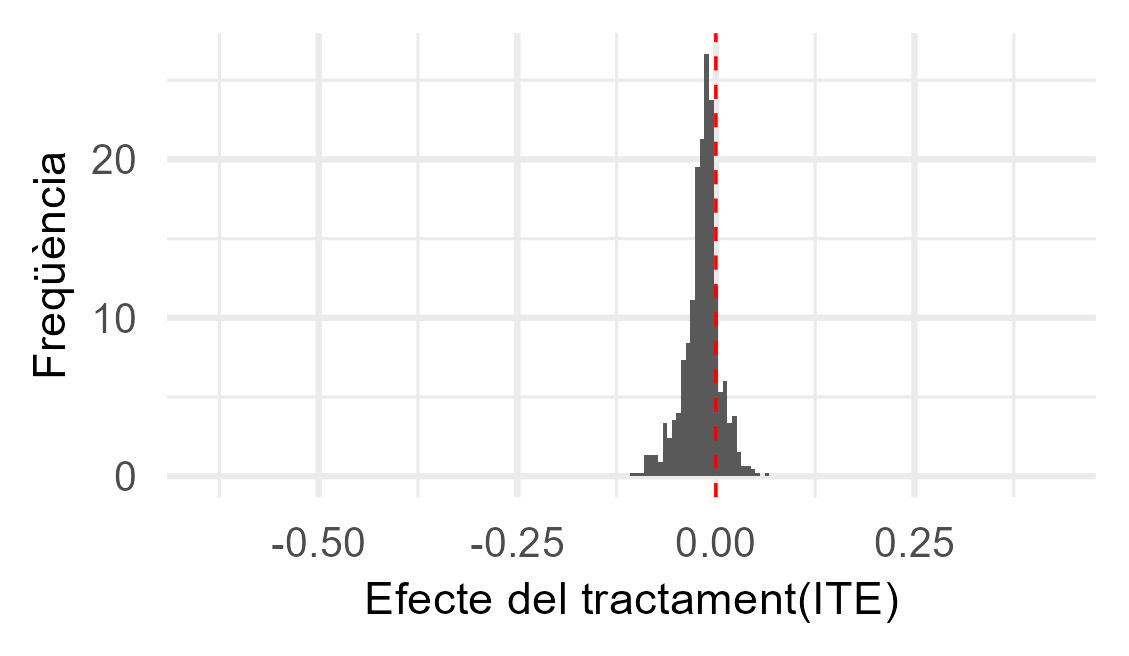
\includegraphics[width=0.3\textwidth]{imgs/histogrames/hist(SGA_prenatal)S_tract2.jpg} &
        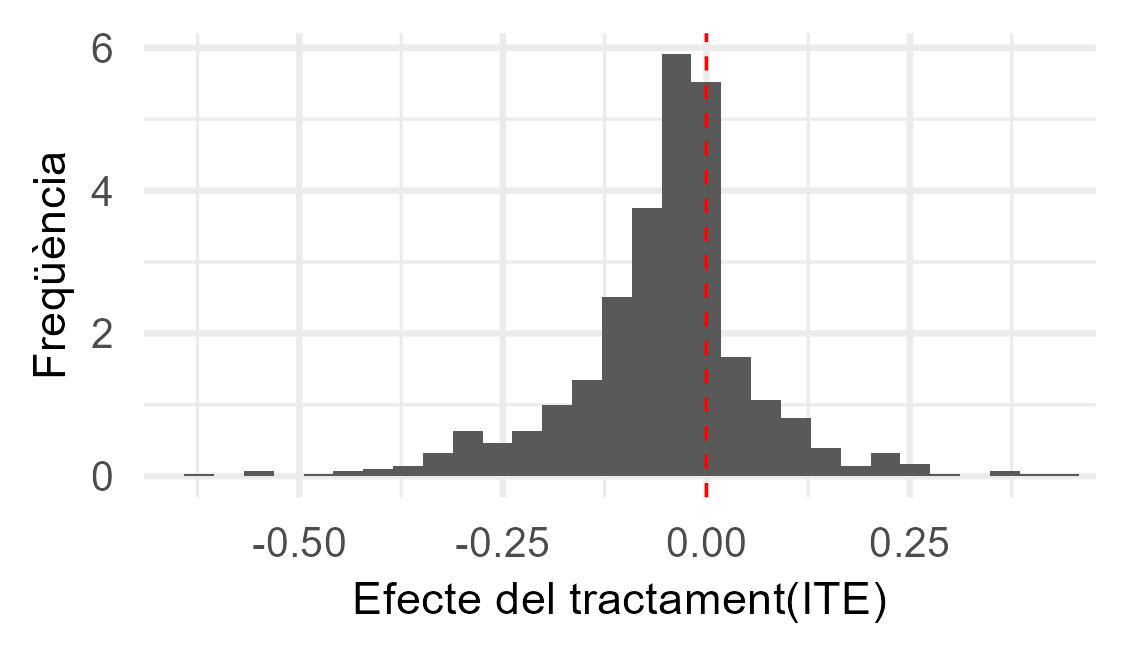
\includegraphics[width=0.3\textwidth]{imgs/histogrames/hist(SGA_prenatal)T_tract2.jpg} &
        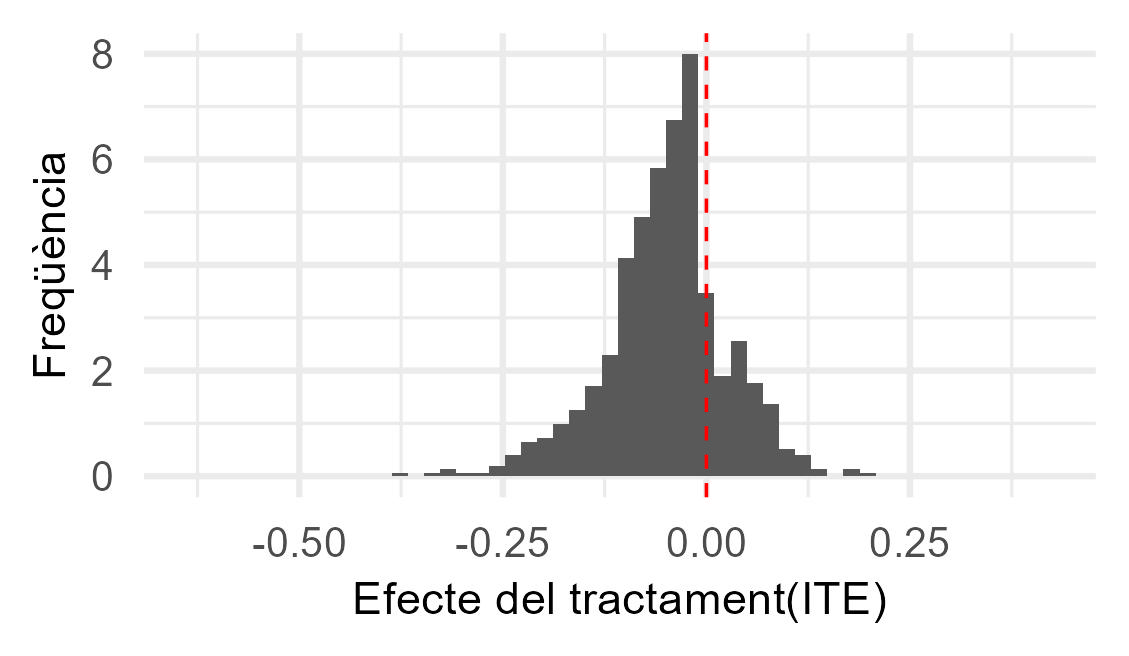
\includegraphics[width=0.3\textwidth]{imgs/histogrames/hist(SGA_prenatal)X_tract2.jpg} \\
        \end{tabular}
        \caption{\footnotesize Comparació visual dels ITEs i ATE estimats amb S-, T- i X-learner per la variable resposta \textit{SGA diagnosticat prenatalment}}
        \label{tab:histITE_prenatSGA2}
    \end{table}

    En analitzar l’efecte del tractament de dieta mediterrània, s’observa una forma de distribució dels ITEs similar a la d’altres outcomes, però amb una lleugera asimetria cap al costat negatiu. Aquesta forma reflecteix que una part de la mostra presenta una resposta més intensa al tractament. L’ATE estimat amb el X-learner és de -0.049, fet que indica que, de mitjana, el tractament redueix en un 4.9\% la probabilitat de diagnòstic prenatal de SGA.
    
    %Mirant l'efecte del tractament amb reducció de l'estrès, una forma similar a les anteriors i s'observa una lleugera assimetria amb més pes de la part negativa. L'ATE estaa a -0.049, es a dir el tractament redueix un 4.9\% la probabilitat de tenir SGA prenatalment. 
    
    \begin{table}[H]
        \centering
        \begin{tabular}{ccc}
        \multicolumn{3}{c}{Histograma de l'ITE amb \textbf{reducció estrès}} \\
        \small \textbf{S-learner} & \small \textbf{T-learner} & \small \textbf{X-learner} \\
        \footnotesize ATE = -0.011 & \footnotesize ATE = -0.028 & \footnotesize ATE = -0.023 \\
        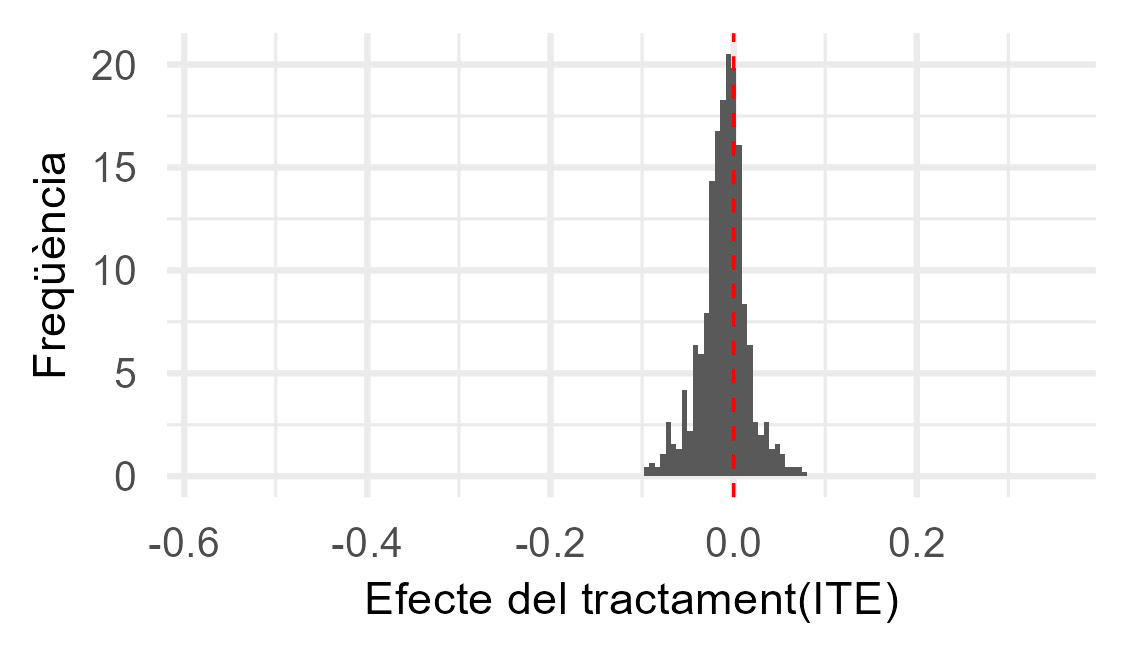
\includegraphics[width=0.3\textwidth]{imgs/histogrames/hist(SGA_prenatal)S_tract3.jpg} &
        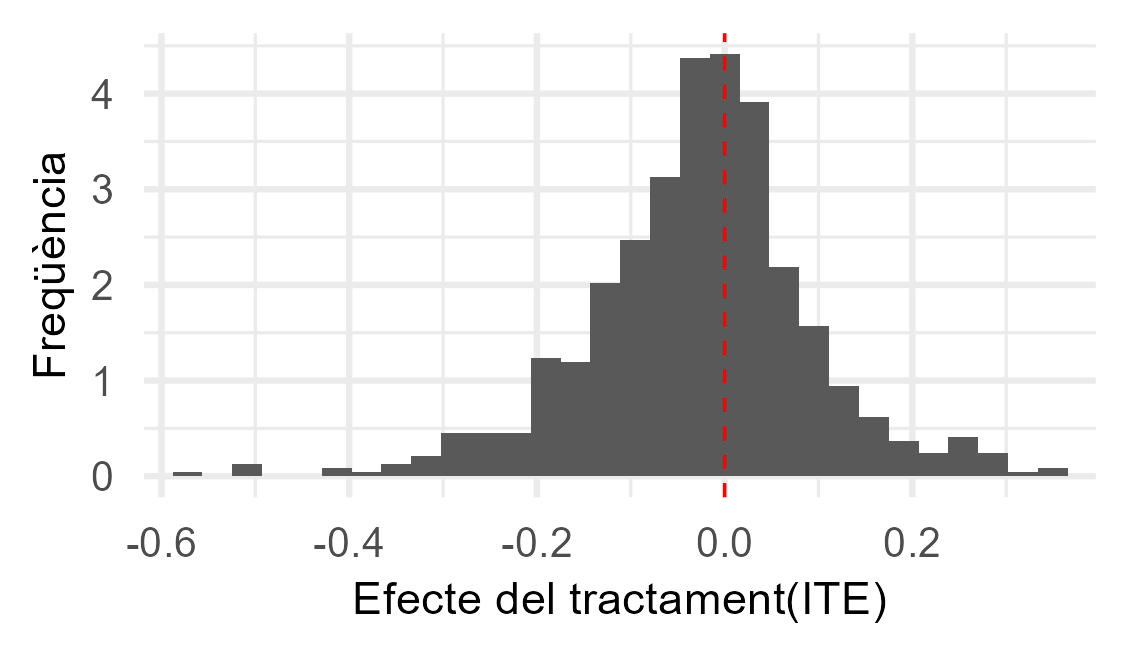
\includegraphics[width=0.3\textwidth]{imgs/histogrames/hist(SGA_prenatal)T_tract3.jpg} &
        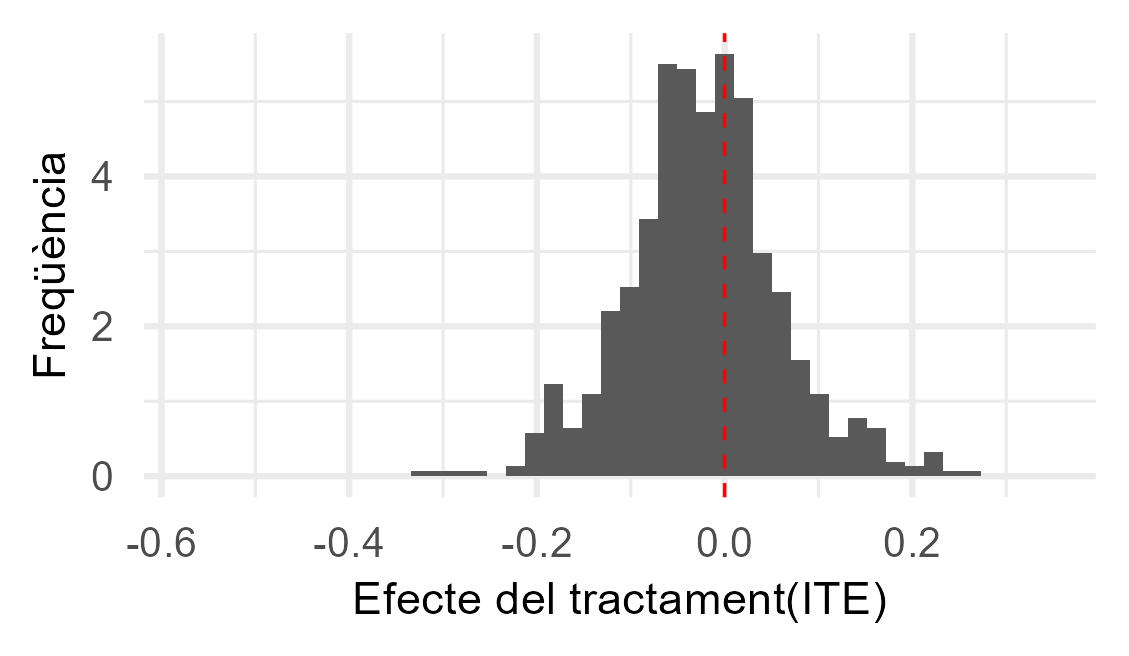
\includegraphics[width=0.3\textwidth]{imgs/histogrames/hist(SGA_prenatal)X_tract3.jpg} \\
        \end{tabular}
        \caption{\footnotesize Comparació visual dels ITEs i ATE estimats amb S-, T- i X-learner per la variable resposta \textit{SGA diagnosticat prenatalment}}
        \label{tab:histITE_prenatSGA3}
    \end{table}

    Pel que fa a la reducció d'estrès, destaca que les distribucions dels ITEs són més simètriques i menys concentrades, amb un pic central menys pronunciat. Això fa que el valor mitjà (ATE) sigui més proper a zero, situant-se en -0.023 amb el X-learner. Tot i que l’efecte global continua sent beneficiós, és més moderat que en el cas del tractament de dieta mediterrània i la menor concentració central suggereix una major heterogeneïtat en la resposta al tractament.



%taula coeficients
    \begin{table}[H]
        \centering
        \captionsetup{font=small}
        \caption{Coeficients estimats i intervals de confiança del model lineal per CATE de SGA prenatal}
        \label{tab:coef_SGAprenat}
        \centering
        \scriptsize
        \begin{tabular}[t]{p{4cm} c @{\hspace{1cm}} c}
        \toprule
        Variable & Tractament  & Tractament \\
         & Dieta mediterrània & Reducció estrès \\
        \midrule
        (Intercept) & \textbf{-0.38 (-0.51; -0.26)} & -0.12 (-0.25; 0.00)\\
        Edat & \textbf{-0.00 (-0.01; -0.00)} & \textbf{0.00 (0.00; 0.00)}\\
        Talla & \textbf{0.00 (0.00; 0.00)} & \textbf{0.00 (0.00; 0.00)}\\
        IMC pregestacional & 0.00 (-0.00; 0.00) & \textbf{-0.00 (-0.00; -0.00)}\\
        Fumadora & 0.02 (-0.02; 0.06) & \textbf{0.06 (0.03; 0.09)}\\
        \addlinespace
        Antecedents SGA & -0.00 (-0.02; 0.01) & \textbf{0.06 (0.05; 0.07)}\\
        HTA crònica & -0.01 (-0.03; 0.02) & -0.01 (-0.04; 0.01)\\
        Diabetis gestacional & 0.01 (-0.02; 0.03) & \textbf{0.03 (0.01; 0.05)}\\
        Nefropatia & \textbf{-0.08 (-0.11; -0.04)} & \textbf{-0.06 (-0.09; -0.03)}\\
        Malaltia autoimmune & \textbf{0.02 (0.00; 0.03)} & \textbf{0.05 (0.03; 0.06)}\\
        \addlinespace
        Doppler patològic & 0.01 (-0.01; 0.03) & -0.00 (-0.02; 0.02)\\
        Risc PE & \textbf{-0.07 (-0.08; -0.06)} & \textbf{-0.03 (-0.04; -0.02)}\\
        PAPP-A patològic & \textbf{-0.03 (-0.05; -0.01)} & \textbf{-0.07 (-0.09; -0.05)}\\
        Metrorràgia & \textbf{-0.04 (-0.06; -0.02)} & \textbf{-0.03 (-0.05; -0.01)}\\
        Criteris SGA & -0.00 (-0.01; 0.01) & \textbf{-0.03 (-0.04; -0.02)}\\
        \addlinespace
        Fecundació assistida & \textbf{0.03 (0.02; 0.04)} & \textbf{0.03 (0.02; 0.05)}\\
        Nul·liparitat & \textbf{0.01 (0.00; 0.02)} & \textbf{-0.04 (-0.05; -0.03)}\\
        \bottomrule
        \multicolumn{3}{l}{\rule{0pt}{1em}*coef (IC$_{95\%}$); \textit{Amb negreta les variables significatives amb $\alpha=0.05$}}
        \end{tabular}
    \end{table}

    A primera vista (taula \ref{tab:coef_SGAprenat}), s’observa que en ambdós tractaments les covariables numèriques (edat, talla i BMI pregestacional), tot i que algunes són estadísticament significatives, tenen efectes pràcticament imperceptibles sobre l’efecte del tractament per al SGA prenatal. En canvi, es detecten patrons més clars en les dones amb \textit{nefropatia}, amb \textit{risc de preeclàmpsia}, amb \textit{nivells patològics de PAPP-A} o amb \textit{metrorràgia} què semblen beneficiar-se més dels tractaments, mostrant una reducció més gran en la probabilitat de SGA prenatal.\par
    Per contra, la presència de \textit{malalties autoimmunitàries} o el fet que l’\textit{embaràs sigui resultat de TRA} es relacionen amb una menor efectivitat dels tractaments, tant per a la reducció de l’estrès com per a la reducció d'estrès.\par
    
    En el cas específic de la \textbf{dieta mediterrània}, s’observa també un efecte lleugerament negatiu associat a la \textit{nul·liparitat}, fet que indica que les mares primerenques responen menys favorablement a aquesta intervenció.\par
    En canvi, en el tractament amb \textbf{reducció d'estrès}, el fet de ser mare primerenca sí que es relaciona amb una major efectivitat del tractament. Això també es dona en embarassos que compleixen \textit{criteris clínics menors de risc de SGA}, on l’efecte és lleugerament més positiu. Tanmateix, en aquest mateix grup de tractament, es detecta una menor efectivitat en mares fumadores, amb antecedents previs de nadons SGA o amb diabetis durant l’embaràs, la qual cosa pot indicar un perfil de resposta més limitada en aquests casos.


    \section{Anàlisi profund del HTE} 
    \label{sec:anal_profun_SGA}
    
    En aquest apartat es proposa dur a terme una anàlisi més detallada i profunda de dos dels outcomes més rellevants de la base de dades: l’SGA al naixement i el pes del nadó al naixement. Aquestes dues variables han estat seleccionades perquè són centrals en l’estudi original (\cite{parct_original}) i, a més, representen dos tipus de variables resposta diferents: una de binària i una de contínua.
    Aquesta elecció permet il·lustrar com es pot estudiar la heterogeneïtat dels efectes del tractament tant en el cas d’un outcome discret com en un de continu. Tanmateix, cal destacar que, com que treballem amb ITE i CATE, valors sempre continus independentment del tipus de variable resposta, la naturalesa original només afectarà en la interpretació dels resultats i l’escala i rang de valors obtinguts.\par
    Per a l’anàlisi detallada de l’HTE en aquestes dues variables s’ha utilitzat un procediment de bootstrap amb 1.000 rèpliques per construir intervals de confiança al voltant de les diferències de CATE entre subgrups. Aquesta metodologia també ha permès comprovar si els intervals incloïen el valor zero, fet que indicaria l’absència de diferències estadísticament significatives entre grups.\par
    En el cas de les variables contínues, s’han ajustat models lineals, prèviament centrant i estandarditzant aquestes variables. Aquesta transformació permet interpretar la magnitud dels coeficients de manera comparable, evitant la influència del rang o escala original.\par
    Finalment, s’han inclòs representacions gràfiques que visualitzen les diferències d’efecte entre subgrups, amb l’objectiu de facilitar la interpretació dels resultats i detectar patrons rellevants d’heterogeneïtat.



    \subsection{HTE amb SGA al naixement com resposta}\label{subsec:profund_SGA}

    De fet l'objectiu principal de l’estudi original és avaluar si els tractaments basats en dieta mediterrània i reducció de l’estrès tenen un impacte positiu sobre el desenvolupament fetal, mesurat a través de la incidència de SGA al naixement. Aquesta variable reflecteix directament la qualitat del creixement intrauterí i s’associa fortament amb la morbiditat i la mortalitat neonatal.\par
    Per aquest motiu, i pel seu significat clínic, utilitzarem aquest outcome com a exemple per dur a terme una anàlisi aprofundida de l’heterogeneïtat de l’efecte del tractament (HTE).\par
    En aquesta secció ens centrarem en els resultats obtinguts amb l’X-learner, que ha mostrat un comportament més robust i fiable, s’ha pogut observat amb les distribucions dels ITEs. Aquest model estima que els tractaments redueixen la probabilitat que el nadó neixi amb SGA en un 7,3\% per a la dieta mediterrània i un 6,1\% per a la reducció de l’estrès.\footnote{L’estudi clínic original estima una reducció del risc del 7,9\% per la dieta mediterrània i del 6,3\% per la reducció de l’estrès.}\par

    Per una banda he calculat l'estimació i els intervals de confiança de les diferències dels CATE de les variables binàries:
    
     \begin{scriptsize}
        \begin{longtable}{lcc}
        \caption{Estimació de la diferència dels CATE i intervals de confiança (variables binàries)} \label{tab:fons_SGA} \\
        \toprule
        Variable & \textbf{Dieta mediterrània} & \textbf{Reducció estrès}\\
        \midrule
        \endfirsthead
        \caption[]{(continuació)} \\
        \toprule
        Variable & \textbf{Dieta mediterrània} & \textbf{Reducció estrès} \\
        \midrule
        \endhead
        \bottomrule
        \multicolumn{3}{l}{\rule{0pt}{1em}CATE(sí) - CATE(no) (IC$_{95\%}$); Amb \textbf{negreta} les els IC que no contenen el 0} \\
        \multicolumn{3}{l}{\rule{0pt}{1em}*\textit{Menys de 2.5\% de casos}; **\textit{Menys de 5\% de casos}} \\
        \endfoot
        %
        Fumadora* & 0.032 (-0.03; 0.11) & \textbf{0.070 (0.04; 0.11)} \\
        \addlinespace
        Antecedents SGA & \textbf{-0.029 (-0.04; -0.02)} & \textbf{0.067 (0.05; 0.08)} \\
        HTA crònica** & \textbf{-0.060 (-0.09; -0.02)} & \textbf{-0.067 (-0.09; -0.04)} \\
        Diabetis gestacional** & \textbf{0.096 (0.07; 0.12)} & \textbf{0.041 (0.01; 0.07)} \\
        Nefropatia & -0.026 (-0.08; 0.02) & 0.002 (-0.03; 0.03) \\
        Malaltia autoimmune & \textbf{0.023 (0.01; 0.04)} & 0.018 (-0.00; 0.04) \\
        \addlinespace
        Doppler patològic & \textbf{0.031 (0.00; 0.06)} & -0.026 (-0.06; 0.02) \\
        Risc PE & \textbf{-0.113 (-0.13; -0.10)} & \textbf{-0.054 (-0.07; -0.04)} \\
        PAPP-A patològic & 0.003 (-0.02; 0.03) & \textbf{-0.097 (-0.12; -0.07)} \\
        Metrorràgia** & 0.001 (-0.03; 0.03) & 0.019 (-0.01; 0.05)\\
        Criteris SGA & \textbf{0.032 (0.02; 0.04)} & -0.010 (-0.02; 0.00) \\
        \addlinespace
        Fecundació assistida & \textbf{0.033 (0.02; 0.05)} & -0.010 (-0.03; 0.01) \\
        Nul·liparitat & \textbf{0.019 (0.01; 0.03)} & \textbf{-0.069 (-0.08; -0.06)} \\
        \end{longtable}
    \end{scriptsize}
    
    Veiem que, pel que fa a l’SGA al naixement, hi ha diverses variables maternes que mostren una heterogeneïtat significativa en l’efecte del tractament. És a dir, la diferència en el CATE entre mares amb i sense determinades característiques és estadísticament significativa, cosa que suggereix que la resposta al tractament no és uniforme entre grups. \par
    El valor de la diferència entre CATEs ens informa sobre la magnitud de l’heterogeneïtat. En interpretar aquest valor cal tenir en compte que ens interessa fer baixar la probabilitat de SGA, per tant:
    \begin{itemize}
        \item Un valor negatiu indica que el tractament beneficia més el subgrup que \textbf{presenta} la característica.
        \item Un valor positiu, en canvi, suggereix que el tractament és més efectiu en el subgrup que \textbf{no presenta} la característica. 
    \end{itemize}

    Les diferències en els CATEs mostren que la dieta mediterrània beneficia especialment les mares amb risc de preeclàmpsia, mentre que l’efecte és menor en mares amb diabetis gestacional (es pot comprobar visualment amb les figures \ref{boxplot:SGA2}). Pel que fa a la reducció de l’estrès, el tractament és més efectiu en mares amb HTA crònica o valors patològics de PAPP-A (a la figura \ref{boxplot:SGA3}), però perd efecte en mares amb antecedents de SGA.
.
    \begin{figure}[!htb]
      \centering
      \begin{minipage}[t]{0.48\textwidth}
        \captionsetup{font=small}
        \caption*{\centering Boxplot dels ITE amb \textbf{dieta mediterrània} segons si la mare ha tingut diabetis durant l'embaràs i si hi ha risc de PE}
        \includegraphics[width=\textwidth]{imgs/boxplots/boxplot_2_SGA.jpg}
        \captionsetup{font=footnotesize}
        \caption{Veiem com la les pacients amb diabetis noten menys l'efecte del tractament mentre que les diagnosticades amb risc de preeclàmpsia es beneficien més de l'efecte de la dieta mediterrània.}
        \label{boxplot:SGA2}
      \end{minipage}
      \hspace{0.01\textwidth}
      \begin{minipage}[t]{0.48\textwidth}
        \captionsetup{font=small}
        \caption*{\centering Boxplot dels ITE amb \textbf{reducció estrès} segons si la mare té antecedents de SGA i si té nivells patològics de PAPP-A}
        \includegraphics[width=\textwidth]{imgs/boxplots/boxplot_3_SGA.jpg}
        \captionsetup{font=footnotesize}
        \caption{Veiem com el tractament amb reducció del estrès va millor per les dones que no tenen antecedents de SGA però beneficia especialment a les que tenen nivells patològics de PAPP-A.}
        \label{boxplot:SGA3}
      \end{minipage}
    \end{figure}

    \begin{figure}[!htb]
      \centering
      \begin{minipage}[t]{0.48\textwidth}
        \captionsetup{font=small}
        \caption*{\centering Boxplot dels ITE amb \textbf{dieta mediterrània} segons edat de la mare}
        \includegraphics[width=\textwidth]{imgs/boxplots/boxplot_edad_2_SGA.jpg}
        \captionsetup{font=footnotesize}
        \caption{La edat guarda certa relació amb els ITE però es molt dèbil, només seria qüestionable la igualtat de l'efecte de la dieta mediterrània entre les més joves i les més grans.}
        \label{boxplot:edat_SGA2}
      \end{minipage}
      \hspace{0.01\textwidth}
      \begin{minipage}[t]{0.48\textwidth}
        \captionsetup{font=small}
        \caption*{\centering Boxplot dels ITE amb \textbf{reducció estrès} segons la talla de la mare}
        \includegraphics[width=\textwidth]{imgs/boxplots/boxplot_talla_3_SGA.jpg}
        \captionsetup{font=footnotesize}
        \caption{En amb aquesta variable si que hi trobem una relació més clara que confirma el signe del coeficient, les mares més altes es beneficien més del tractament de reducció de l'estrès.}
        \label{boxplot:talla_SGA3}
      \end{minipage}
    \end{figure}

    Per analitzar com es relacionen les variables contínues amb l’efecte del tractament, cal modificar l’enfocament analític, ja que no disposem de categories discretes com en el cas de les variables binàries. Una opció consisteix a transformar les variables contínues en intervals, per exemple mitjançant trencaments per percentils (com es fa a les figures \ref{boxplot:edat_SGA2} i \ref{boxplot:talla_SGA3}). No obstant això, aquesta aproximació pot comportar pèrdua d’informació.\par
    Des del punt de vista estadístic, la manera més robusta i informativa d’avaluar aquestes relacions és mitjançant una regressió lineal dels ITEs sobre les covariables contínues. Aquesta tècnica permet estimar la direcció i la intensitat de l’associació a partir dels coeficients del model i la seva significació estadística, tal com s’ha aplicat anteriorment. però a diferencia d'abans aplicarem aquest model utilitzant les variables numèriques centrades i escalades. Tot i que això fa que els coeficients no siguin directament interpretables en unitats originals, sí que ens permet comparar la magnitud relativa dels efectes i entendre el signe de la relació de manera coherent.

    
    
    \begin{table}[H]
        \centering
        \captionsetup{font=small}
        \caption{Coeficients estimats i intervals de confiança del model lineal per ITE al SGA al naixement}
        \label{tab:prof_coef_SGA}
        \centering
        \scriptsize
        \begin{tabular}[t]{p{4cm} c @{\hspace{1cm}} c}
        \toprule
        Variable & Tractament  & Tractament \\
         & Dieta mediterrània & Reducció estrès \\
        \midrule
        Edat & \textbf{0.01 (0.01; 0.02)} & \textbf{0.03 (0.03; 0.04)}\\
        Talla & \textbf{-0.01 (-0.01; -0.00)} & \textbf{-0.04 (-0.04; -0.03)}\\
        IMC pregestacional & \textbf{0.01 (0.01; 0.02)} & \textbf{-0.01 (-0.01; -0.00)}\\
        \bottomrule
        \multicolumn{3}{l}{\rule{0pt}{1em}*coef (IC$_{95\%}$); \textit{Amb \textbf{negreta} les variables significatives amb $\alpha=0.05$}}
        \end{tabular}
    \end{table}

    Veiem que tots els coeficients són significatius, però en el cas de la dieta mediterrània són molt petits. Cal recordar que ara les variables estan centrades i escalades. A més, la visualització de les gràfiques que relacionen cadascuna d’aquestes variables amb els ITE sembla que no guardin cap relació clara. Així, tot sembla indicar que les tres variables numèriques tenen una relació molt lleu amb els ITE. Tot i que no són característiques menyspreables, no constitueixen una font important d’heterogeneïtat de l’efecte del tractament.\par
    En canvi, en el cas del tractament de reducció de l’estrès sí que sembla haver-hi una relació més rellevant entre l’efecte del tractament i tant la talla com l’edat. A mesura que augmenta l’altura, també ho fa l’efecte del tractament, i al contrari, com més gran és l’edat, menor és l’efecte beneficiós del tractament.\par
    
    
    




    \subsection{HTE amb pes del recent nascut com resposta}
    \label{subsec:profund_pes}
    El pes al naixement, no és la variable resposta principal de l'estudi d'on provenen les dades però també s'analitza i s'en destaca la rellevança. És clau per avaluar el desenvolupament intrauterí i s’ha associat àmpliament amb la salut neonatal immediata i amb el risc de complicacions futures. Un pes més elevat s’interpreta generalment com un indicador d’una gestació favorable, i per tant, en aquest context, considerarem beneficiosos aquells efectes del tractament que incrementin el pes al naixement.\par
    Segons les estimacions de l’X-learner, l’ATE associat al tractament de dieta mediterrània és de 92,8 grams guanyats respecte al grup control, mentre que el de reducció de l’estrès és lleugerament superior, amb un increment mitjà de 95,53 grams. Aquests resultats indiquen que ambdós tractaments tenen un efecte positiu i clínicament rellevant sobre el pes del nadó al naixement.\par
    Seguint el mateix enfocament que amb l’SGA al naixement, a continuació analitzem les diferències en els CATEs entre els diferents nivells de les variables binàries, amb l’objectiu d’identificar possibles patrons d’heterogeneïtat en l’efecte del tractament sobre el pes al naixement.

    \begin{scriptsize}
        \begin{longtable}{lcc}
        \caption{Estimació de la diferència dels CATE i intervals de confiança (variables binàries)} \label{tab:fons_pes} \\
        \toprule
        Variable & \textbf{Dieta mediterrània} & \textbf{Reducció estrès}\\
        \midrule
        \endfirsthead
        \caption[]{(continuació)} \\
        \toprule
        Variable & \textbf{Dieta mediterrània} & \textbf{Reducció estrès} \\
        \midrule
        \endhead
        \bottomrule
        \multicolumn{3}{l}{\rule{0pt}{1em}CATE(sí) - CATE(no) (IC$_{95\%}$); Amb \textbf{negreta} les els IC que no contenen el 0} \\
        \multicolumn{3}{l}{\rule{0pt}{1em}*\textit{Menys de 2.5\% de casos}; **\textit{Menys de 5\% de casos}} \\
        \endfoot
        %
        Fumadora* & -64.78 (-171.9; 44.5) & -54.35 (-137.1; 31.0) \\
        \addlinespace
        Antecedents SGA & \textbf{-22.69 (-42.6; -1.5)} & \textbf{-58.11 (-79.5; -38.0)} \\
        HTA crònica** & \textbf{139.98 (90.8; 196.4)} & -28.95 (-73.5; 18.1) \\
        Diabetis gestacional** & 14.48 (-23.7; 52.0) & 27.22 (-23.6; 80.2) \\
        Nefropatia & 3.24 (-53.7; 60.8) & 37.05 (-26.1; 96.8) \\
        Malaltia autoimmune & \textbf{-72.67 (-101.1; -45.6)} & -14.16 (-42.2; 14.2) \\
        \addlinespace
        Doppler patològic & \textbf{-162.27 (-203.3; -121.9)} & \textbf{-123.44 (-165.0; -84.0)} \\
        Risc PE & \textbf{92.25 (73.6; 114.5)} & 6.42 (-16.8; 28.0) \\
        PAPP-A patològic & 7.07 (-35.1; 47.4) & \textbf{89.99 (48.4; 131.9)} \\
        Metrorràgia** & \textbf{-187.85 (-234.8; -143.3)} & \textbf{-65.90 (-113.5; -20.6)}\\
        Criteris SGA & \textbf{23.05 (3.1; 44.2)} & \textbf{51.71 (32.9; 70.9)} \\
        \addlinespace
        Fecundació assistida & -2.06 (-24.2; 19.5) & -6.66 (-31.2; 17.7) \\
        Nul·liparitat & 5.11 (-14.3; 26.4) & \textbf{74.87 (57.1; 93.5)} \\
        \end{longtable}
    \end{scriptsize}

    S’observa que, en aquest outcome, hi ha menys variables que generen heterogeneïtat significativa en l’efecte del tractament. Cal tenir en compte que, en aquest cas, el resultat estimat fa referència a grams de diferència en el pes al naixement entre subgrups. És a dir, les diferències de CATE indiquen quant augmenta (o disminueix) el pes com a efecte del tractament en mares amb una determinada característica respecte a les que no la tenen. Per aixó:
    \begin{itemize}
        \item Un valor negatiu indica que el tractament és més efectiu en el subgrup que \textbf{no presenta} la característica: és a dir, l’increment de pes és superior en aquest grup. 
        \item Un valor positiu indica que el tractament afavoreix més el subgrup que \textbf{presenta} la característica. 
    \end{itemize}

    L’anàlisi de les diferències de CATE mostra que, entre altres variables significatives, la dieta mediterrània incrementa especialment el pes al naixement en nadons de mares amb hipertensió arterial crònica i en aquelles diagnosticades amb risc de preeclàmpsia. Per contra, l’efecte del tractament es redueix de manera significativa en mares amb resultats patològics en l’ecografia Doppler del primer trimestre i en aquelles que han patit metrorràgia durant l’embaràs (veure figura \ref{plot:peso2}), és a dir, el tractament beneficia més les mares que no presenten aquestes condicions.\par
    Pel que fa al tractament de reducció de l’estrès, destaca negativament el cas de les mares amb diagnòstic patològic a l’ecografia Doppler, igual que amb l'altre tractament els seus nadons no experimenten un augment de pes tan notable com els de les mares sense aquest diagnòstic. En canvi, el tractament és especialment beneficiós en mares amb valors patològics de la proteïna PAPP-A, que mostren un guany de pes més gran respecte a les que no presenten aquesta patologia.\par
    Cal destacar que hi ha variables que presenten un patró d’efecte similar en ambdós tractaments. Ja s’ha observat que les mares amb resultats patològics a l’ecografia Doppler es beneficien especialment tant de la dieta mediterrània com de la reducció de l’estrès. El mateix patró s’identifica en les mares que compleixen criteris clínics menors de risc d’SGA, les quals experimenten un augment més gran del pes al naixement amb tots dos tractaments. Finalment, les mares sense antecedents de SGA i les que no han patit metrorràgia durant l’embaràs també es beneficien de manera més clara que les que sí dels efectes de les dues intervencions.

    \begin{figure}[!htb]
      \centering
      \begin{minipage}[t]{0.48\textwidth}
        \captionsetup{font=small}
        \caption*{\centering Boxplot dels ITE amb \textbf{dieta mediterrània} segons si la mare ha tingut metrorràgia i si hi ha risc de PE}
        \includegraphics[width=\textwidth]{imgs/boxplots/boxplot_2_pes.jpg}
        \captionsetup{font=footnotesize}
        \caption{Les mares que han tingut metrorràgia han notat menys els efectes de la dieta mediterrània mentre que els embarassos amb risc de preeclàmpsia s'han beneficiat més que els que no tenien aquesta diagnosis.}
        \label{boxplot:pes2}
      \end{minipage}
      \hspace{0.01\textwidth}
      \begin{minipage}[t]{0.48\textwidth}
        \captionsetup{font=small}
        \caption*{\centering Boxplot dels ITE amb \textbf{reducció estrès} segons si la mare  té nivells patològics de PAPP-A}
        \includegraphics[width=\textwidth]{imgs/boxplots/boxplot_3_pes.jpg}
        \captionsetup{font=footnotesize}
        \caption{En el tractament de la reducció de l'estrès veiem com les mares amb nivells patològics de PAPP-A han tingut un efecte més elevat del tractament. Però les diagnosticades amb alguna patologia a l'ecografia de Doppler noten menys els efectes del tractament que aquelles que no.}
        \label{boxplot:pes3}
      \end{minipage}
    \end{figure}

    \begin{figure}[!htb]
      \centering
      \begin{minipage}[t]{0.48\textwidth}
        \captionsetup{font=small}
        \caption*{\centering Boxplot dels ITE amb \textbf{dieta mediterrània} segons edat de la mare}
        \includegraphics[width=\textwidth]{imgs/boxplots/boxplot_edad_2_pes.jpg}
        \captionsetup{font=footnotesize}
        \caption{Hi ha una relació lleugerament positiva del pes i l'efecte de la dieta mediterrània, a més edat més pes. Sobretot es nota un petit increment a les mares de 37-40 anys respecte les més joves.}
        \label{boxplot:edat_pes2}
      \end{minipage}
      \hspace{0.01\textwidth}
      \begin{minipage}[t]{0.48\textwidth}
        \captionsetup{font=small}
        \caption*{\centering Boxplot dels ITE amb \textbf{reducció estrès} segons la talla de la mare}
        \includegraphics[width=\textwidth]{imgs/boxplots/boxplot_talla_3_pes.jpg}
        \captionsetup{font=footnotesize}
        \caption{La talla de les mares sembla estar clarament relacionada amb l’efecte del tractament: a més alçada, major efecte sobre el pes. S’observa un augment progressiu tant de la mediana com de la dispersió dels ITEs.}
        \label{boxplot:talla_pes3}
      \end{minipage}
    \end{figure}
    
    I si ara ens fixem amb les variables continues utilitzant els coeficients del model lineal amb les variables numeriques centrades i escalades com amb l'exemple anterior veiem:
    \begin{table}[H]
        \centering
        \captionsetup{font=small}
        \caption{Coeficients estimats i intervals de confiança del model lineal per ITE al pes al naixement}
        \label{tab:prof_coef_pes}
        \centering
        \scriptsize
        \begin{tabular}[t]{p{4cm} c @{\hspace{1cm}} c}
        \toprule
        Variable & Tractament  & Tractament \\
         & Dieta mediterrània & Reducció estrès \\
        \midrule
        Edat & \textbf{31.64 (22.51; 40.77)} & \textbf{27.96 (18.93; 36.98)}\\
        Talla & \textbf{23.26 (15.08; 31.44)} & \textbf{41.09 (33.03; 49.15)}\\
        IMC pregestac & \textbf{12.72 (4.33; 21.11)} & \textbf{16.89 (8.71; 25.06)}\\
        \bottomrule
        \multicolumn{3}{l}{\rule{0pt}{1em}*coef (IC$_{95\%}$); \textit{Amb \textbf{negreta} les variables significatives amb $\alpha=0.05$}}
        \end{tabular}
    \end{table}

    Les tres variables numèriques analitzades —edat, talla i BMI pregestacional— presenten coeficients positius i estadísticament significatius en ambdós tractaments. Això indica que, com més elevats són els valors d’aquestes variables, major és l’efecte estimat del tractament sobre el pes al naixement.
    En el cas de la dieta mediterrània, destaca especialment l’edat materna, mentre que en el de la reducció de l’estrès ho fa la talla. Aquestes dues variables són les que mostren una major magnitud de coeficient, i per tant, són les que contribueixen més clarament a la heterogeneïtat de l’efecte del tractament en cada cas. Això es pot visualitzar de manera clara a les figures corresponents (vegeu figures \ref{boxplot:edat_pes2} i \ref{boxplot:talla_pes3}).    
    

    \section{Aplicació Shiny}

    També s’ha dissenyat una aplicació Shiny en R que permet realitzar una anàlisi interactiva i ràpida: des de la visualització dels ITEs amb histogrames fins a l’estimació mitjançant l’X-learner, l’exploració dels CATE per subgrups i el resum dels coeficients d’un model lineal ajustat amb totes les covariables. A més, l’aplicació incorpora una funcionalitat per predir l’ITE d’una nova observació, introduint manualment els valors de les seves variables explicatives.
    
    \begin{figure}[!h]
        \centering
        \includegraphics[width=0.9\linewidth]{imgs/pestanya1_shiny.jpg}
        \caption{Pàgina d’inici de l’aplicació Shiny}
    \end{figure}
    
    Per utilitzar l’aplicació, primer cal seleccionar la variable resposta i el tractament a analitzar (sobre els quals es calcularan els ITEs). Un cop feta la selecció, es prem el botó per entrenar el model. Quan el model ha estat entrenat, apareixen les opcions per introduir les característiques de la nova pacient i calcular el seu ITE.\par
    
    Les funcionalitats principals de l’aplicació es divideixen en tres pestanyes:
    \begin{enumerate}
        \item \textbf{Predicció individual:} mostra el valor de l’ITE per a la nova observació (si s’han introduït les seves característiques) i un histograma amb la distribució dels ITEs de tota la mostra.
        
        \item \textbf{Anàlisi per subgrups:} permet seleccionar una covariable binària i calcula els CATE corresponents a cada grup, amb els seus intervals de confiança estimats mitjançant bootstrap (1.000 rèpliques). També es mostra un comentari amb la proporció d’individus amb valor "Sí" en la mostra i sobre si els intervals de confiança se solapen, per valorar possibles diferències d’efecte entre grups. A més, apareix un boxplot dels ITE de la mateixa variable.
    
        \item \textbf{Model lineal:} presenta una taula amb els coeficients i intervals de confiança de totes les 16 variables explicatives, segons el model lineal ajustat a partir dels ITEs, tal com s’ha fet a l’anàlisi de l’HTE dels diferents outcomes.
    \end{enumerate}
    
    Aquesta aplicació té una aplicabilitat clara, ja que permet tant recomanar o no un tractament a noves pacients, com també explorar de manera senzilla l’heterogeneïtat dels efectes del tractament.
    
    L’aplicació i el seu codi complet són accessibles al \href{https://github.com/jordi-lr/tfg-inferencia_causal}{repositori GitHub del treball}. A més, a l’annex s’hi adjunten captures de pantalla de les diferents pestanyes.


    
    \FloatBarrier
    \section{Conclusions}\label{sec:concl_parct}


   \paragraph{Sobre les variables analitzades amb profunditat} Donada la seva importància clínica, aquests dos outcomes han estat analitzats amb més profunditat que la resta. En el cas del \textbf{SGA al naixement}, s’ha observat que diverses característiques maternes dicotòmiques —com la diabetis durant l’embaràs, el diagnòstic de risc de preeclàmpsia o la hipertensió arterial crònica— generen una heterogeneïtat destacada en l’efecte de la dieta mediterrània. En canvi, les variables contínues com l’edat, la talla i el BMI pregestacional no mostren una relació tan clara amb aquest tractament.\par
    Pel que fa a la reducció de l’estrès, s’ha constatat que el seu efecte varia significativament en funció de si la mare presenta hipertensió crònica, risc de preeclàmpsia o ha patit metrorràgia. A diferència de la dieta mediterrània, aquest tractament sí que mostra una relació més forta amb les variables contínues, especialment l’edat i la talla.\par
    En relació amb el \textbf{pes al naixement}, s’ha identificat que la hipertensió crònica, la detecció de patologia a l’ecografia Doppler del primer trimestre, el risc de preeclàmpsia i la metrorràgia influeixen notablement en l’efecte de la dieta mediterrània. Tot i que les variables contínues, l'edat i la talla, també tenen un paper, el seu impacte és més suau.\par
    En canvi, quan el tractament és la reducció de l’estrès, la heterogeneïtat de l’efecte sobre el pes al naixement ve determinada principalment per variables com els valors patològics de PAPP-A i la diagnosi amb l'ecogràfica de Doppler. En aquest cas, les variables contínues, sobretot talla i edat, mostren una relació més clara amb l'efecte, mentre que la majoria de binàries generen diferències menys marcades entre subgrups.\par
    En conjunt, ambdós outcomes mostren com diverses característiques maternes modulen l’efectivitat dels tractaments, tot i que els dos tractament tinguin patrons diferents en l'HTE també hi ha algunes coincidències. I destaca el fet que les variables contínues, especialment l’edat i la talla, tenen un paper molt més rellevant en la heterogeneïtat de l’efecte del tractament de reducció de l’estrès que en el de la dieta mediterrània amb els dos outcomes.

    
    
    \paragraph{Sobre l'HTE} Els resultats obtinguts mitjançant models lineals que regressaven els ITEs mostren de manera clara que l'efecte del tractament és heterogeni, i depèn tant de les característiques clíniques i demogràfiques de la mare com del tipus d'outcome considerat. Aquesta heterogeneïtat es fa evident també des del punt de vista visual a les figures \ref{plot:SGAnaix2}, \ref{plot:peso2}, \ref{plot:SGAgreu3} i \ref{plot:PE3}, on es poden observar patrons diferenciats de resposta al tractament segons el perfil matern.
    
    \begin{figure}[H]
      \centering
      \begin{minipage}[t]{0.48\textwidth}
        \captionsetup{font=small}
        \caption*{\centering ITE en el pes del nounat amb tractament de \textbf{dieta mediterrània} en funció de l'\textit{edat} diferenciant per \textit{metrorràgia}}
        \includegraphics[width=\textwidth]{imgs/scaterplots/scater_PesoRN_2_EdadMetrorragia.jpg}
        \captionsetup{font=footnotesize}
        \caption{El gràfic sembla indicar que les mares amb metrorràgia noten menys els efectes beneficiós del tractament, gairebé tots els casos tenen ITE nuls o negatius. En canvi, sembla haver una relació positiva entre l'edat i l'efecte del tractament, les mares més grans noten més l'efecte del tractament en el pes del seu fill.}
        \label{plot:peso2}
      \end{minipage}
      \hspace{0.01\textwidth}
      \begin{minipage}[t]{0.48\textwidth}
        \captionsetup{font=small}
        \caption*{\centering ITE en el SGA al naixment amb tractament de \textbf{dieta mediterrània} en funció de \textit{talla} diferenciant per \textit{risc de PE}}
        \includegraphics[width=\textwidth]{imgs/scaterplots/scater_SGAnaix_2_TallaRiscPE.jpg}
        \captionsetup{font=footnotesize}
        \caption{Es mostra com els casos amb risc de PE positiu tenen un efecte més beneficiós que els que no (la majoria de punts tenen ITE negatiu) amb el tractament de mediterrània. També hi ha una lleugera tendència negativa pel que fa a la talla cosa que beneficia lleugerament a les mares més altes.}
        \label{plot:SGAnaix2}
      \end{minipage}
    \end{figure}

    \begin{figure}[H]
      \centering
      \begin{minipage}[t]{0.48\textwidth}
        \captionsetup{font=small}
        \caption*{\centering ITE en el SGA greu amb tractament de \textbf{reducció estrès} en funció de l'\textit{talla} diferenciant per \textit{hipertensió arterial crònica}}
        \includegraphics[width=\textwidth]{imgs/scaterplots/scater_SGAgreu_3_TallaHTAcr.jpg}
        \captionsetup{font=footnotesize}
        \caption{Es mostra com la talla redueix l'efecte del tractament, en canvi el subgrup amb hipertensió es beneficien molt més de la reducció d'estrès que els que no, tenen un efecte del tractament més negatiu.}
        \label{plot:SGAgreu3}
      \end{minipage}
      \hspace{0.01\textwidth}
      \begin{minipage}[t]{0.48\textwidth}
        \captionsetup{font=small}
        \caption*{\centering ITE en el preeclàmpsia amb tractament de \textbf{reducció estrès} en funció de \textit{BMI} diferenciant per \textit{embaràs concebut amb TRA}}
        \includegraphics[width=\textwidth]{imgs/scaterplots/scater_PE_3_BMI_TRA.jpg}
        \captionsetup{font=footnotesize}
        \caption{Pel que fa al BMI s'ha de tenir en compte que els valors més extrems poden fer de punts palanca per al regressió, però s'observa un salt cap a més efecte del tractament a partir del BMI 30. Pel que fa al fet de ser un embaràs concebut amb TRA la informació visual del gràfic i el coeficient al model lineal evidencien un efecte suau que millorà l'efecte del tractament.}
        \label{plot:PE3}
      \end{minipage}
    \end{figure}


    
    \paragraph{Sobre l’aplicabilitat individual de les prediccions} Les anàlisis per subgrups, com les desenvolupades a la secció \ref{sec:analHTE} i \ref{sec:anal_profun_SGA}, són metodològicament robustes i interpretables, i constitueixen una base sòlida per fer recomanacions clíniques preliminars. A més, si la mostra ho permet també es pot fer subgrups combinant diferents covariables.\par
    Tanmateix, les estimacions generades pels models de meta-learning poden ser utilitzades per orientar decisions terapèutiques individualitzades en mares futures. En estimar els CATE i ATE s’han emprat ITEs calculats a partir de les covariables maternes; per tant, és possible fer prediccions per a noves pacients si les seves característiques són comparables a les de la mostra d’estudi i aquesta és suficientment representativa de la població objectiu.\par
    Encara que aquesta aplicació individual només és vàlida sota certes assumpcions metodològiques clau, com ara la ignorabilitat (no hi ha confusió no observada) i la positivitat (tota pacient té una probabilitat positiva de rebre qualsevol tractament). A més, cal tenir present que la ITE és una quantitat no observable i estimada amb incertesa, especialment en regions de l'espai de covariables amb baixa densitat de mostres, on la validesa externa és baixa.\par
    En el nostre cas, si es treballa amb mares que presenten característiques similars a les de la població estudiada i es compleixen les propietats esmentades, es poden fer prediccions dels ITEs per ajudar a decidir si recomanar o no un tractament determinat. Aquesta predicció es pot dur a terme amb qualsevol dels tres meta-learners, tot i que, atenent al rendiment observat al llarg de l’estudi, és recomanable utilitzar l’X-learner. Utilitzant les característiques del nou pacient com a nova $x$, el procediment seria el següent:
    \begin{itemize}
        \item \textbf{Amb S-learner}: S'utilitzaria l'únic model per preveure els dos potencials, amb i sense tractament,  i amb la diferència és calcularia l'ITE ($\hat{\mu}(x,T=1)-\hat{\mu}(x,T=0)$).
        \item \textbf{Amb T-learner}: S'utilitzaria els dos models $\hat\mu_0(x)$ i $\hat\mu_1(x)$ per calcular els potencials i després fer la diferencia que serà el ITE.
        \item \textbf{Amb X-learner}: Es fa servir la combinació ponderada dels dos models finals de $\hat\tau_0$ i $\hat\tau_1$ per fer les prediccions i calcular $g(x)\hat\tau_1+(1-g(x))\hat\tau_0(x)$ on $g(x)$ fa referencia al propensity score que un context de decisió individualitzada (on es vol determinar quin tractament aplicar), té sentit fixar $g(x) = 0.5$, assumint que el pacient podria rebre qualsevol dels dos tractaments amb la mateixa probabilitat.
    \end{itemize}

    \FloatBarrier
    \paragraph{Sobre les variables amb pocs casos} Cal actuar amb precaució a l’hora d’interpretar els resultats associats a certes variables amb baixa freqüència en la mostra, com ara el tabaquisme, la nefropatia o la hipertensió arterial crònica, les quals no superen el 5\% de casos positius. Aquesta escassetat pot donar lloc a relacions espúries o poc robustes estadísticament. A més, és important remarcar que aquest estudi s’ha concebut com a exploratori utilitzant dades d'un experiment amb uns objectius diferents, i per tal de poder generalitzar les conclusions obtingudes seria necessari dissenyar un nou assaig específic, orientat a avaluar l’impacte d’aquestes variables en la resposta al tractament.\par
    Encara que alguns resultats s’hagin d’interpretar amb cautela, no resta valor ni rellevància a les conclusions globals del treball. En efecte, s’ha pogut confirmar l’efecte positiu dels tractaments en la majoria dels outcomes analitzats, així com la presència d’efectes heterogenis, és a dir, que la resposta al tractament no és homogènia per a totes les pacients, fet que reforça la utilitat d’un enfocament personalitzat.
    
    \paragraph{Sobre els meta-learners} Abans d’analitzar els efectes heterogenis del tractament, convé destacar que les diferències observades entre els ATEs estimats amb el T-learner i l’X-learner no són estadísticament significatives, si es té en compte la variabilitat dels ITEs. Tot i això, s’ha pogut constatar que el T-learner tendeix a generar estimacions més disperses, amb una variància considerablement més elevada, fet que fa perdre fiabilitat.\par
    Pel que fa a l’S-learner, els resultats obtinguts mostren un rendiment clarament inferior, especialment en situacions amb relacions no lineals complexes o outcomes amb baixa incidència. En la majoria de casos, l’S-learner ha generat valors d’ITE molt propers a zero i amb molt poca variabilitat, el què suggereix una capacitat limitada per capturar la heterogeneïtat real dels efectes individuals.

    \paragraph{Sobre la comparació dels ATE} Al llarg de l’anàlisi també s’han detectat diferències entre els ATEs estimats per als dos tractaments (reducció de l’estrès i reducció d'estrès). Tot i això, cal fer dues consideracions importants:\par
    Primer, aquesta comparació no és l’objectiu principal del treball, i per extreure conclusions significatives caldria aplicar els mètodes per comparar aquests dos tractaments, o utilitzar contrastos d’hipòtesis o intervals de confiança per a la diferència d’ATEs.\par
    Segon, la variància dels ITEs dins de cada tractament és prou elevada com per considerar que les diferències observades en els ATEs, excepte en algun cas puntual, no són estadísticament significatives (mirant els intervals de confiança).

    


    


\end{document}